\documentclass[twoside]{book}

% Packages required by doxygen
\usepackage{fixltx2e}
\usepackage{calc}
\usepackage{doxygen}
\usepackage[export]{adjustbox} % also loads graphicx
\usepackage{graphicx}
\usepackage[utf8]{inputenc}
\usepackage{makeidx}
\usepackage{multicol}
\usepackage{multirow}
\PassOptionsToPackage{warn}{textcomp}
\usepackage{textcomp}
\usepackage[nointegrals]{wasysym}
\usepackage[table]{xcolor}

% Font selection
\usepackage[T1]{fontenc}
\usepackage[scaled=.90]{helvet}
\usepackage{courier}
\usepackage{amssymb}
\usepackage{sectsty}
\renewcommand{\familydefault}{\sfdefault}
\allsectionsfont{%
  \fontseries{bc}\selectfont%
  \color{darkgray}%
}
\renewcommand{\DoxyLabelFont}{%
  \fontseries{bc}\selectfont%
  \color{darkgray}%
}
\newcommand{\+}{\discretionary{\mbox{\scriptsize$\hookleftarrow$}}{}{}}

% Page & text layout
\usepackage{geometry}
\geometry{%
  a4paper,%
  top=2.5cm,%
  bottom=2.5cm,%
  left=2.5cm,%
  right=2.5cm%
}
\tolerance=750
\hfuzz=15pt
\hbadness=750
\setlength{\emergencystretch}{15pt}
\setlength{\parindent}{0cm}
\setlength{\parskip}{0.2cm}
\makeatletter
\renewcommand{\paragraph}{%
  \@startsection{paragraph}{4}{0ex}{-1.0ex}{1.0ex}{%
    \normalfont\normalsize\bfseries\SS@parafont%
  }%
}
\renewcommand{\subparagraph}{%
  \@startsection{subparagraph}{5}{0ex}{-1.0ex}{1.0ex}{%
    \normalfont\normalsize\bfseries\SS@subparafont%
  }%
}
\makeatother

% Headers & footers
\usepackage{fancyhdr}
\pagestyle{fancyplain}
\fancyhead[LE]{\fancyplain{}{\bfseries\thepage}}
\fancyhead[CE]{\fancyplain{}{}}
\fancyhead[RE]{\fancyplain{}{\bfseries\leftmark}}
\fancyhead[LO]{\fancyplain{}{\bfseries\rightmark}}
\fancyhead[CO]{\fancyplain{}{}}
\fancyhead[RO]{\fancyplain{}{\bfseries\thepage}}
\fancyfoot[LE]{\fancyplain{}{}}
\fancyfoot[CE]{\fancyplain{}{}}
\fancyfoot[RE]{\fancyplain{}{\bfseries\scriptsize Generated on Tue Dec 29 2015 15\+:08\+:43 for Switch-\/\+Compiler by Doxygen }}
\fancyfoot[LO]{\fancyplain{}{\bfseries\scriptsize Generated on Tue Dec 29 2015 15\+:08\+:43 for Switch-\/\+Compiler by Doxygen }}
\fancyfoot[CO]{\fancyplain{}{}}
\fancyfoot[RO]{\fancyplain{}{}}
\renewcommand{\footrulewidth}{0.4pt}
\renewcommand{\chaptermark}[1]{%
  \markboth{#1}{}%
}
\renewcommand{\sectionmark}[1]{%
  \markright{\thesection\ #1}%
}

% Indices & bibliography
\usepackage{natbib}
\usepackage[titles]{tocloft}
\setcounter{tocdepth}{3}
\setcounter{secnumdepth}{5}
\makeindex

% Hyperlinks (required, but should be loaded last)
\usepackage{ifpdf}
\ifpdf
  \usepackage[pdftex,pagebackref=true]{hyperref}
\else
  \usepackage[ps2pdf,pagebackref=true]{hyperref}
\fi
\hypersetup{%
  colorlinks=true,%
  linkcolor=blue,%
  citecolor=blue,%
  unicode%
}

% Custom commands
\newcommand{\clearemptydoublepage}{%
  \newpage{\pagestyle{empty}\cleardoublepage}%
}


%===== C O N T E N T S =====

\begin{document}

% Titlepage & ToC
\hypersetup{pageanchor=false,
             bookmarks=true,
             bookmarksnumbered=true,
             pdfencoding=unicode
            }
\pagenumbering{roman}
\begin{titlepage}
\vspace*{7cm}
\begin{center}%
{\Large Switch-\/\+Compiler \\[1ex]\large 1.\+0 }\\
\vspace*{1cm}
{\large Generated by Doxygen 1.8.10}\\
\vspace*{0.5cm}
{\small Tue Dec 29 2015 15:08:43}\\
\end{center}
\end{titlepage}
\clearemptydoublepage
\tableofcontents
\clearemptydoublepage
\pagenumbering{arabic}
\hypersetup{pageanchor=true}

%--- Begin generated contents ---
\chapter{Hierarchical Index}
\section{Class Hierarchy}
This inheritance list is sorted roughly, but not completely, alphabetically\+:\begin{DoxyCompactList}
\item \contentsline{section}{mapper.\+src.\+flexpipe.\+flexpipe\+\_\+configuration.\+Flexpipe\+Configuration}{\pageref{classmapper_1_1src_1_1flexpipe_1_1flexpipe__configuration_1_1_flexpipe_configuration}}{}
\item \contentsline{section}{mapper.\+src.\+flexpipe.\+flexpipe\+\_\+dependency\+\_\+analysis.\+Flexpipe\+Dependency\+Analysis}{\pageref{classmapper_1_1src_1_1flexpipe_1_1flexpipe__dependency__analysis_1_1_flexpipe_dependency_analysis}}{}
\item \contentsline{section}{mapper.\+src.\+flexpipe.\+flexpipe\+\_\+ilp\+\_\+compiler.\+Flexpipe\+Ilp\+Compiler}{\pageref{classmapper_1_1src_1_1flexpipe_1_1flexpipe__ilp__compiler_1_1_flexpipe_ilp_compiler}}{}
\item \contentsline{section}{mapper.\+src.\+flexpipe.\+flexpipe\+\_\+lpt\+\_\+compiler.\+Flexpipe\+Lpt\+Compiler}{\pageref{classmapper_1_1src_1_1flexpipe_1_1flexpipe__lpt__compiler_1_1_flexpipe_lpt_compiler}}{}
\item \contentsline{section}{mapper.\+src.\+flexpipe.\+flexpipe\+\_\+preprocess.\+Flexpipe\+Preprocess}{\pageref{classmapper_1_1src_1_1flexpipe_1_1flexpipe__preprocess_1_1_flexpipe_preprocess}}{}
\item \contentsline{section}{mapper.\+src.\+flexpipe.\+flexpipe\+\_\+switch.\+Flexpipe\+Switch}{\pageref{classmapper_1_1src_1_1flexpipe_1_1flexpipe__switch_1_1_flexpipe_switch}}{}
\item \contentsline{section}{mapper.\+src.\+rmt.\+rmt\+\_\+configuration.\+Rmt\+Configuration}{\pageref{classmapper_1_1src_1_1rmt_1_1rmt__configuration_1_1_rmt_configuration}}{}
\item \contentsline{section}{mapper.\+src.\+rmt.\+rmt\+\_\+dependency\+\_\+analysis.\+Rmt\+Dependency\+Analysis}{\pageref{classmapper_1_1src_1_1rmt_1_1rmt__dependency__analysis_1_1_rmt_dependency_analysis}}{}
\item \contentsline{section}{mapper.\+src.\+rmt.\+rmt\+\_\+greedy\+\_\+compiler.\+Rmt\+Greedy\+Compiler}{\pageref{classmapper_1_1src_1_1rmt_1_1rmt__greedy__compiler_1_1_rmt_greedy_compiler}}{}
\item \contentsline{section}{mapper.\+src.\+rmt.\+orig\+\_\+rmt\+\_\+compiler.\+Rmt\+Ilp\+Compiler}{\pageref{classmapper_1_1src_1_1rmt_1_1orig__rmt__compiler_1_1_rmt_ilp_compiler}}{}
\item \contentsline{section}{mapper.\+src.\+rmt.\+rmt\+\_\+preprocess.\+Rmt\+Preprocess}{\pageref{classmapper_1_1src_1_1rmt_1_1rmt__preprocess_1_1_rmt_preprocess}}{}
\item \contentsline{section}{mapper.\+src.\+rmt.\+rmt\+\_\+switch.\+Rmt\+Switch}{\pageref{classmapper_1_1src_1_1rmt_1_1rmt__switch_1_1_rmt_switch}}{}
\item Rmt\+Greedy\+Compiler\begin{DoxyCompactList}
\item \contentsline{section}{mapper.\+src.\+rmt.\+rmt\+\_\+ffd\+\_\+compiler.\+Rmt\+Ffd\+Compiler}{\pageref{classmapper_1_1src_1_1rmt_1_1rmt__ffd__compiler_1_1_rmt_ffd_compiler}}{}
\item \contentsline{section}{mapper.\+src.\+rmt.\+rmt\+\_\+ffl\+\_\+compiler.\+Rmt\+Ffl\+Compiler}{\pageref{classmapper_1_1src_1_1rmt_1_1rmt__ffl__compiler_1_1_rmt_ffl_compiler}}{}
\item \contentsline{section}{mapper.\+src.\+rmt.\+rmt\+\_\+ffls\+\_\+compiler.\+Rmt\+Ffls\+Compiler}{\pageref{classmapper_1_1src_1_1rmt_1_1rmt__ffls__compiler_1_1_rmt_ffls_compiler}}{}
\end{DoxyCompactList}
\end{DoxyCompactList}

\chapter{Class Index}
\section{Class List}
Here are the classes, structs, unions and interfaces with brief descriptions\+:\begin{DoxyCompactList}
\item\contentsline{section}{\hyperlink{classmapper_1_1src_1_1flexpipe_1_1flexpipe__configuration_1_1_flexpipe_configuration}{mapper.\+src.\+flexpipe.\+flexpipe\+\_\+configuration.\+Flexpipe\+Configuration} }{\pageref{classmapper_1_1src_1_1flexpipe_1_1flexpipe__configuration_1_1_flexpipe_configuration}}{}
\item\contentsline{section}{\hyperlink{classmapper_1_1src_1_1flexpipe_1_1flexpipe__dependency__analysis_1_1_flexpipe_dependency_analysis}{mapper.\+src.\+flexpipe.\+flexpipe\+\_\+dependency\+\_\+analysis.\+Flexpipe\+Dependency\+Analysis} }{\pageref{classmapper_1_1src_1_1flexpipe_1_1flexpipe__dependency__analysis_1_1_flexpipe_dependency_analysis}}{}
\item\contentsline{section}{\hyperlink{classmapper_1_1src_1_1flexpipe_1_1flexpipe__ilp__compiler_1_1_flexpipe_ilp_compiler}{mapper.\+src.\+flexpipe.\+flexpipe\+\_\+ilp\+\_\+compiler.\+Flexpipe\+Ilp\+Compiler} }{\pageref{classmapper_1_1src_1_1flexpipe_1_1flexpipe__ilp__compiler_1_1_flexpipe_ilp_compiler}}{}
\item\contentsline{section}{\hyperlink{classmapper_1_1src_1_1flexpipe_1_1flexpipe__lpt__compiler_1_1_flexpipe_lpt_compiler}{mapper.\+src.\+flexpipe.\+flexpipe\+\_\+lpt\+\_\+compiler.\+Flexpipe\+Lpt\+Compiler} }{\pageref{classmapper_1_1src_1_1flexpipe_1_1flexpipe__lpt__compiler_1_1_flexpipe_lpt_compiler}}{}
\item\contentsline{section}{\hyperlink{classmapper_1_1src_1_1flexpipe_1_1flexpipe__preprocess_1_1_flexpipe_preprocess}{mapper.\+src.\+flexpipe.\+flexpipe\+\_\+preprocess.\+Flexpipe\+Preprocess} }{\pageref{classmapper_1_1src_1_1flexpipe_1_1flexpipe__preprocess_1_1_flexpipe_preprocess}}{}
\item\contentsline{section}{\hyperlink{classmapper_1_1src_1_1flexpipe_1_1flexpipe__switch_1_1_flexpipe_switch}{mapper.\+src.\+flexpipe.\+flexpipe\+\_\+switch.\+Flexpipe\+Switch} }{\pageref{classmapper_1_1src_1_1flexpipe_1_1flexpipe__switch_1_1_flexpipe_switch}}{}
\item\contentsline{section}{\hyperlink{classmapper_1_1src_1_1rmt_1_1rmt__configuration_1_1_rmt_configuration}{mapper.\+src.\+rmt.\+rmt\+\_\+configuration.\+Rmt\+Configuration} }{\pageref{classmapper_1_1src_1_1rmt_1_1rmt__configuration_1_1_rmt_configuration}}{}
\item\contentsline{section}{\hyperlink{classmapper_1_1src_1_1rmt_1_1rmt__dependency__analysis_1_1_rmt_dependency_analysis}{mapper.\+src.\+rmt.\+rmt\+\_\+dependency\+\_\+analysis.\+Rmt\+Dependency\+Analysis} }{\pageref{classmapper_1_1src_1_1rmt_1_1rmt__dependency__analysis_1_1_rmt_dependency_analysis}}{}
\item\contentsline{section}{\hyperlink{classmapper_1_1src_1_1rmt_1_1rmt__ffd__compiler_1_1_rmt_ffd_compiler}{mapper.\+src.\+rmt.\+rmt\+\_\+ffd\+\_\+compiler.\+Rmt\+Ffd\+Compiler} }{\pageref{classmapper_1_1src_1_1rmt_1_1rmt__ffd__compiler_1_1_rmt_ffd_compiler}}{}
\item\contentsline{section}{\hyperlink{classmapper_1_1src_1_1rmt_1_1rmt__ffl__compiler_1_1_rmt_ffl_compiler}{mapper.\+src.\+rmt.\+rmt\+\_\+ffl\+\_\+compiler.\+Rmt\+Ffl\+Compiler} }{\pageref{classmapper_1_1src_1_1rmt_1_1rmt__ffl__compiler_1_1_rmt_ffl_compiler}}{}
\item\contentsline{section}{\hyperlink{classmapper_1_1src_1_1rmt_1_1rmt__ffls__compiler_1_1_rmt_ffls_compiler}{mapper.\+src.\+rmt.\+rmt\+\_\+ffls\+\_\+compiler.\+Rmt\+Ffls\+Compiler} }{\pageref{classmapper_1_1src_1_1rmt_1_1rmt__ffls__compiler_1_1_rmt_ffls_compiler}}{}
\item\contentsline{section}{\hyperlink{classmapper_1_1src_1_1rmt_1_1rmt__greedy__compiler_1_1_rmt_greedy_compiler}{mapper.\+src.\+rmt.\+rmt\+\_\+greedy\+\_\+compiler.\+Rmt\+Greedy\+Compiler} }{\pageref{classmapper_1_1src_1_1rmt_1_1rmt__greedy__compiler_1_1_rmt_greedy_compiler}}{}
\item\contentsline{section}{\hyperlink{classmapper_1_1src_1_1rmt_1_1orig__rmt__compiler_1_1_rmt_ilp_compiler}{mapper.\+src.\+rmt.\+orig\+\_\+rmt\+\_\+compiler.\+Rmt\+Ilp\+Compiler} }{\pageref{classmapper_1_1src_1_1rmt_1_1orig__rmt__compiler_1_1_rmt_ilp_compiler}}{}
\item\contentsline{section}{\hyperlink{classmapper_1_1src_1_1rmt_1_1rmt__preprocess_1_1_rmt_preprocess}{mapper.\+src.\+rmt.\+rmt\+\_\+preprocess.\+Rmt\+Preprocess} }{\pageref{classmapper_1_1src_1_1rmt_1_1rmt__preprocess_1_1_rmt_preprocess}}{}
\item\contentsline{section}{\hyperlink{classmapper_1_1src_1_1rmt_1_1rmt__switch_1_1_rmt_switch}{mapper.\+src.\+rmt.\+rmt\+\_\+switch.\+Rmt\+Switch} }{\pageref{classmapper_1_1src_1_1rmt_1_1rmt__switch_1_1_rmt_switch}}{}
\end{DoxyCompactList}

\chapter{Class Documentation}
\hypertarget{classmapper_1_1src_1_1flexpipe_1_1flexpipe__configuration_1_1_flexpipe_configuration}{}\section{mapper.\+src.\+flexpipe.\+flexpipe\+\_\+configuration.\+Flexpipe\+Configuration Class Reference}
\label{classmapper_1_1src_1_1flexpipe_1_1flexpipe__configuration_1_1_flexpipe_configuration}\index{mapper.\+src.\+flexpipe.\+flexpipe\+\_\+configuration.\+Flexpipe\+Configuration@{mapper.\+src.\+flexpipe.\+flexpipe\+\_\+configuration.\+Flexpipe\+Configuration}}
\subsection*{Public Member Functions}
\begin{DoxyCompactItemize}
\item 
\hypertarget{classmapper_1_1src_1_1flexpipe_1_1flexpipe__configuration_1_1_flexpipe_configuration_ad1477f2b84c0a34090a04f01d159fd8d}{}def {\bfseries \+\_\+\+\_\+init\+\_\+\+\_\+} (self, program, switch, preprocess, version)\label{classmapper_1_1src_1_1flexpipe_1_1flexpipe__configuration_1_1_flexpipe_configuration_ad1477f2b84c0a34090a04f01d159fd8d}

\item 
\hypertarget{classmapper_1_1src_1_1flexpipe_1_1flexpipe__configuration_1_1_flexpipe_configuration_a9abef61c74b66b9bbb4ebb6e52bcfd4f}{}def {\bfseries display\+Initial\+Conditions} (self)\label{classmapper_1_1src_1_1flexpipe_1_1flexpipe__configuration_1_1_flexpipe_configuration_a9abef61c74b66b9bbb4ebb6e52bcfd4f}

\item 
def \hyperlink{classmapper_1_1src_1_1flexpipe_1_1flexpipe__configuration_1_1_flexpipe_configuration_a353b2acd97a6bbeac04f12113cab92a0}{get\+Per\+Log\+Assign\+Info} (self)
\item 
def \hyperlink{classmapper_1_1src_1_1flexpipe_1_1flexpipe__configuration_1_1_flexpipe_configuration_a5b0d9a6c6ec1d34da8c0ced0e7ffdd90}{get\+Earliest\+Stage\+From\+Assign} (self, assign\+Info)
\item 
\hypertarget{classmapper_1_1src_1_1flexpipe_1_1flexpipe__configuration_1_1_flexpipe_configuration_a9d60b71bcd41989ea56581e8b309965f}{}def {\bfseries configure} (self, start\+Row, number\+Of\+Rows)\label{classmapper_1_1src_1_1flexpipe_1_1flexpipe__configuration_1_1_flexpipe_configuration_a9d60b71bcd41989ea56581e8b309965f}

\item 
def \hyperlink{classmapper_1_1src_1_1flexpipe_1_1flexpipe__configuration_1_1_flexpipe_configuration_a7a42a167b54bbcf85f1c26ead6593d11}{display} (self)
\item 
\hypertarget{classmapper_1_1src_1_1flexpipe_1_1flexpipe__configuration_1_1_flexpipe_configuration_a305b089197866964769330cc4d49f733}{}def {\bfseries get\+Colors\+From\+Table\+Groups} (self, table\+Groups)\label{classmapper_1_1src_1_1flexpipe_1_1flexpipe__configuration_1_1_flexpipe_configuration_a305b089197866964769330cc4d49f733}

\item 
\hypertarget{classmapper_1_1src_1_1flexpipe_1_1flexpipe__configuration_1_1_flexpipe_configuration_ae6eba8d6597aae8dda93346589466de0}{}def {\bfseries show\+Pic}\label{classmapper_1_1src_1_1flexpipe_1_1flexpipe__configuration_1_1_flexpipe_configuration_ae6eba8d6597aae8dda93346589466de0}

\end{DoxyCompactItemize}
\subsection*{Public Attributes}
\begin{DoxyCompactItemize}
\item 
\hypertarget{classmapper_1_1src_1_1flexpipe_1_1flexpipe__configuration_1_1_flexpipe_configuration_a828d4e3e977cfc19211fc5bbb6651779}{}{\bfseries logger}\label{classmapper_1_1src_1_1flexpipe_1_1flexpipe__configuration_1_1_flexpipe_configuration_a828d4e3e977cfc19211fc5bbb6651779}

\item 
\hypertarget{classmapper_1_1src_1_1flexpipe_1_1flexpipe__configuration_1_1_flexpipe_configuration_a785d620989004a35e974e0be16095cf5}{}{\bfseries program}\label{classmapper_1_1src_1_1flexpipe_1_1flexpipe__configuration_1_1_flexpipe_configuration_a785d620989004a35e974e0be16095cf5}

\item 
\hypertarget{classmapper_1_1src_1_1flexpipe_1_1flexpipe__configuration_1_1_flexpipe_configuration_a9b7b17b210172a4b393ed7b0d324d527}{}{\bfseries switch}\label{classmapper_1_1src_1_1flexpipe_1_1flexpipe__configuration_1_1_flexpipe_configuration_a9b7b17b210172a4b393ed7b0d324d527}

\item 
\hypertarget{classmapper_1_1src_1_1flexpipe_1_1flexpipe__configuration_1_1_flexpipe_configuration_abfc77b5ff6390612a5c828b6ea05e9ce}{}{\bfseries preprocess}\label{classmapper_1_1src_1_1flexpipe_1_1flexpipe__configuration_1_1_flexpipe_configuration_abfc77b5ff6390612a5c828b6ea05e9ce}

\item 
\hypertarget{classmapper_1_1src_1_1flexpipe_1_1flexpipe__configuration_1_1_flexpipe_configuration_a2be554f54c2c563cbc608344d3478514}{}{\bfseries version}\label{classmapper_1_1src_1_1flexpipe_1_1flexpipe__configuration_1_1_flexpipe_configuration_a2be554f54c2c563cbc608344d3478514}

\item 
\hypertarget{classmapper_1_1src_1_1flexpipe_1_1flexpipe__configuration_1_1_flexpipe_configuration_a2b73e64979a69d8935aa7a7721179a17}{}{\bfseries da}\label{classmapper_1_1src_1_1flexpipe_1_1flexpipe__configuration_1_1_flexpipe_configuration_a2b73e64979a69d8935aa7a7721179a17}

\item 
\hypertarget{classmapper_1_1src_1_1flexpipe_1_1flexpipe__configuration_1_1_flexpipe_configuration_a2b8227101fd01848931a568ad5efc158}{}{\bfseries st\+Max}\label{classmapper_1_1src_1_1flexpipe_1_1flexpipe__configuration_1_1_flexpipe_configuration_a2b8227101fd01848931a568ad5efc158}

\item 
\hypertarget{classmapper_1_1src_1_1flexpipe_1_1flexpipe__configuration_1_1_flexpipe_configuration_a278200d3867af8d8fc8c0cb6bf453ba4}{}{\bfseries log\+Max}\label{classmapper_1_1src_1_1flexpipe_1_1flexpipe__configuration_1_1_flexpipe_configuration_a278200d3867af8d8fc8c0cb6bf453ba4}

\item 
\hypertarget{classmapper_1_1src_1_1flexpipe_1_1flexpipe__configuration_1_1_flexpipe_configuration_aaa6ad95be7de2883f8ea99aae6d32652}{}{\bfseries start\+Row}\label{classmapper_1_1src_1_1flexpipe_1_1flexpipe__configuration_1_1_flexpipe_configuration_aaa6ad95be7de2883f8ea99aae6d32652}

\item 
\hypertarget{classmapper_1_1src_1_1flexpipe_1_1flexpipe__configuration_1_1_flexpipe_configuration_a8eedd555cf60e861037add1d3c40a146}{}{\bfseries number\+Of\+Rows}\label{classmapper_1_1src_1_1flexpipe_1_1flexpipe__configuration_1_1_flexpipe_configuration_a8eedd555cf60e861037add1d3c40a146}

\item 
\hypertarget{classmapper_1_1src_1_1flexpipe_1_1flexpipe__configuration_1_1_flexpipe_configuration_a3d3f96fa7bdda1fb05e13f03dce5c5d2}{}{\bfseries color\+Names}\label{classmapper_1_1src_1_1flexpipe_1_1flexpipe__configuration_1_1_flexpipe_configuration_a3d3f96fa7bdda1fb05e13f03dce5c5d2}

\end{DoxyCompactItemize}


\subsection{Detailed Description}
\begin{DoxyVerb}Module to describe and log a FlexPipe switch configuration
for a given program
\end{DoxyVerb}
 

\subsection{Member Function Documentation}
\hypertarget{classmapper_1_1src_1_1flexpipe_1_1flexpipe__configuration_1_1_flexpipe_configuration_a7a42a167b54bbcf85f1c26ead6593d11}{}\index{mapper\+::src\+::flexpipe\+::flexpipe\+\_\+configuration\+::\+Flexpipe\+Configuration@{mapper\+::src\+::flexpipe\+::flexpipe\+\_\+configuration\+::\+Flexpipe\+Configuration}!display@{display}}
\index{display@{display}!mapper\+::src\+::flexpipe\+::flexpipe\+\_\+configuration\+::\+Flexpipe\+Configuration@{mapper\+::src\+::flexpipe\+::flexpipe\+\_\+configuration\+::\+Flexpipe\+Configuration}}
\subsubsection[{display(self)}]{\setlength{\rightskip}{0pt plus 5cm}def mapper.\+src.\+flexpipe.\+flexpipe\+\_\+configuration.\+Flexpipe\+Configuration.\+display (
\begin{DoxyParamCaption}
\item[{}]{self}
\end{DoxyParamCaption}
)}\label{classmapper_1_1src_1_1flexpipe_1_1flexpipe__configuration_1_1_flexpipe_configuration_a7a42a167b54bbcf85f1c26ead6593d11}
\begin{DoxyVerb}Display configuration- tables in each memory type,
in each stage.
\end{DoxyVerb}
 \hypertarget{classmapper_1_1src_1_1flexpipe_1_1flexpipe__configuration_1_1_flexpipe_configuration_a5b0d9a6c6ec1d34da8c0ced0e7ffdd90}{}\index{mapper\+::src\+::flexpipe\+::flexpipe\+\_\+configuration\+::\+Flexpipe\+Configuration@{mapper\+::src\+::flexpipe\+::flexpipe\+\_\+configuration\+::\+Flexpipe\+Configuration}!get\+Earliest\+Stage\+From\+Assign@{get\+Earliest\+Stage\+From\+Assign}}
\index{get\+Earliest\+Stage\+From\+Assign@{get\+Earliest\+Stage\+From\+Assign}!mapper\+::src\+::flexpipe\+::flexpipe\+\_\+configuration\+::\+Flexpipe\+Configuration@{mapper\+::src\+::flexpipe\+::flexpipe\+\_\+configuration\+::\+Flexpipe\+Configuration}}
\subsubsection[{get\+Earliest\+Stage\+From\+Assign(self, assign\+Info)}]{\setlength{\rightskip}{0pt plus 5cm}def mapper.\+src.\+flexpipe.\+flexpipe\+\_\+configuration.\+Flexpipe\+Configuration.\+get\+Earliest\+Stage\+From\+Assign (
\begin{DoxyParamCaption}
\item[{}]{self, }
\item[{}]{assign\+Info}
\end{DoxyParamCaption}
)}\label{classmapper_1_1src_1_1flexpipe_1_1flexpipe__configuration_1_1_flexpipe_configuration_a5b0d9a6c6ec1d34da8c0ced0e7ffdd90}
\begin{DoxyVerb}Returns a mapping from tables
to information about the first stage they could have started
in- a table must start after all the tables it depends on
have been completely assigned. The informations is a list of
 lists [@st, @dep, @prev, @prevEnd] which should be read as        
Table xx can't start before stage @st because of @dependency
on table @prev which ends in stage @prevEnd, one for each
@prev that the table depends on.
\end{DoxyVerb}
 \hypertarget{classmapper_1_1src_1_1flexpipe_1_1flexpipe__configuration_1_1_flexpipe_configuration_a353b2acd97a6bbeac04f12113cab92a0}{}\index{mapper\+::src\+::flexpipe\+::flexpipe\+\_\+configuration\+::\+Flexpipe\+Configuration@{mapper\+::src\+::flexpipe\+::flexpipe\+\_\+configuration\+::\+Flexpipe\+Configuration}!get\+Per\+Log\+Assign\+Info@{get\+Per\+Log\+Assign\+Info}}
\index{get\+Per\+Log\+Assign\+Info@{get\+Per\+Log\+Assign\+Info}!mapper\+::src\+::flexpipe\+::flexpipe\+\_\+configuration\+::\+Flexpipe\+Configuration@{mapper\+::src\+::flexpipe\+::flexpipe\+\_\+configuration\+::\+Flexpipe\+Configuration}}
\subsubsection[{get\+Per\+Log\+Assign\+Info(self)}]{\setlength{\rightskip}{0pt plus 5cm}def mapper.\+src.\+flexpipe.\+flexpipe\+\_\+configuration.\+Flexpipe\+Configuration.\+get\+Per\+Log\+Assign\+Info (
\begin{DoxyParamCaption}
\item[{}]{self}
\end{DoxyParamCaption}
)}\label{classmapper_1_1src_1_1flexpipe_1_1flexpipe__configuration_1_1_flexpipe_configuration_a353b2acd97a6bbeac04f12113cab92a0}
\begin{DoxyVerb} Return mapping from table to assignment info
  'start': start stage (or -1 if not valid)
  'end': end stage (or -1 if not valid)
\end{DoxyVerb}
 

The documentation for this class was generated from the following file\+:\begin{DoxyCompactItemize}
\item 
src/flexpipe/flexpipe\+\_\+configuration.\+py\end{DoxyCompactItemize}

\hypertarget{classmapper_1_1src_1_1flexpipe_1_1flexpipe__dependency__analysis_1_1_flexpipe_dependency_analysis}{}\section{mapper.\+src.\+flexpipe.\+flexpipe\+\_\+dependency\+\_\+analysis.\+Flexpipe\+Dependency\+Analysis Class Reference}
\label{classmapper_1_1src_1_1flexpipe_1_1flexpipe__dependency__analysis_1_1_flexpipe_dependency_analysis}\index{mapper.\+src.\+flexpipe.\+flexpipe\+\_\+dependency\+\_\+analysis.\+Flexpipe\+Dependency\+Analysis@{mapper.\+src.\+flexpipe.\+flexpipe\+\_\+dependency\+\_\+analysis.\+Flexpipe\+Dependency\+Analysis}}
\subsection*{Public Member Functions}
\begin{DoxyCompactItemize}
\item 
\hypertarget{classmapper_1_1src_1_1flexpipe_1_1flexpipe__dependency__analysis_1_1_flexpipe_dependency_analysis_a403e4f2346834b4f7ee764dbbeccd59b}{}def {\bfseries \+\_\+\+\_\+init\+\_\+\+\_\+} (self, program)\label{classmapper_1_1src_1_1flexpipe_1_1flexpipe__dependency__analysis_1_1_flexpipe_dependency_analysis_a403e4f2346834b4f7ee764dbbeccd59b}

\item 
\hypertarget{classmapper_1_1src_1_1flexpipe_1_1flexpipe__dependency__analysis_1_1_flexpipe_dependency_analysis_aed014630950f2bcc7e0fb947c4a87088}{}def {\bfseries get\+Digraph} (self)\label{classmapper_1_1src_1_1flexpipe_1_1flexpipe__dependency__analysis_1_1_flexpipe_dependency_analysis_aed014630950f2bcc7e0fb947c4a87088}

\item 
\hypertarget{classmapper_1_1src_1_1flexpipe_1_1flexpipe__dependency__analysis_1_1_flexpipe_dependency_analysis_a672d87478af539ba387d466960f9fe06}{}def {\bfseries get\+Digraph\+From\+Start\+Negative} (self)\label{classmapper_1_1src_1_1flexpipe_1_1flexpipe__dependency__analysis_1_1_flexpipe_dependency_analysis_a672d87478af539ba387d466960f9fe06}

\item 
\hypertarget{classmapper_1_1src_1_1flexpipe_1_1flexpipe__dependency__analysis_1_1_flexpipe_dependency_analysis_ac6b8b644d559284ce18a4426d3a37761}{}def {\bfseries make\+Path} (self, nodes, gr)\label{classmapper_1_1src_1_1flexpipe_1_1flexpipe__dependency__analysis_1_1_flexpipe_dependency_analysis_ac6b8b644d559284ce18a4426d3a37761}

\item 
\hypertarget{classmapper_1_1src_1_1flexpipe_1_1flexpipe__dependency__analysis_1_1_flexpipe_dependency_analysis_a15324f645ecd56d24f59487d15c9fb4c}{}def {\bfseries show\+Path}\label{classmapper_1_1src_1_1flexpipe_1_1flexpipe__dependency__analysis_1_1_flexpipe_dependency_analysis_a15324f645ecd56d24f59487d15c9fb4c}

\item 
\hypertarget{classmapper_1_1src_1_1flexpipe_1_1flexpipe__dependency__analysis_1_1_flexpipe_dependency_analysis_a1b56743a3791cee38f05fc46522424fc}{}def {\bfseries get\+Per\+Log\+Program\+Info} (self)\label{classmapper_1_1src_1_1flexpipe_1_1flexpipe__dependency__analysis_1_1_flexpipe_dependency_analysis_a1b56743a3791cee38f05fc46522424fc}

\item 
\hypertarget{classmapper_1_1src_1_1flexpipe_1_1flexpipe__dependency__analysis_1_1_flexpipe_dependency_analysis_acf4db83c5f44a03069f1d45e1d0a55ed}{}def {\bfseries get\+Digraph\+From\+End\+Positive} (self)\label{classmapper_1_1src_1_1flexpipe_1_1flexpipe__dependency__analysis_1_1_flexpipe_dependency_analysis_acf4db83c5f44a03069f1d45e1d0a55ed}

\item 
\hypertarget{classmapper_1_1src_1_1flexpipe_1_1flexpipe__dependency__analysis_1_1_flexpipe_dependency_analysis_ae636e37d774f03946d8e10885a05ca5a}{}def {\bfseries get\+Digraph\+From\+Start\+Positive} (self)\label{classmapper_1_1src_1_1flexpipe_1_1flexpipe__dependency__analysis_1_1_flexpipe_dependency_analysis_ae636e37d774f03946d8e10885a05ca5a}

\item 
\hypertarget{classmapper_1_1src_1_1flexpipe_1_1flexpipe__dependency__analysis_1_1_flexpipe_dependency_analysis_a1512fb4e2f30235d017282104cbcde0b}{}def {\bfseries show\+Critical\+Path} (self)\label{classmapper_1_1src_1_1flexpipe_1_1flexpipe__dependency__analysis_1_1_flexpipe_dependency_analysis_a1512fb4e2f30235d017282104cbcde0b}

\end{DoxyCompactItemize}
\subsection*{Public Attributes}
\begin{DoxyCompactItemize}
\item 
\hypertarget{classmapper_1_1src_1_1flexpipe_1_1flexpipe__dependency__analysis_1_1_flexpipe_dependency_analysis_a42d048d684101817d06e190a4f459d10}{}{\bfseries logger}\label{classmapper_1_1src_1_1flexpipe_1_1flexpipe__dependency__analysis_1_1_flexpipe_dependency_analysis_a42d048d684101817d06e190a4f459d10}

\item 
\hypertarget{classmapper_1_1src_1_1flexpipe_1_1flexpipe__dependency__analysis_1_1_flexpipe_dependency_analysis_a00e4fa144fe632800624ed3b5ec34224}{}{\bfseries program}\label{classmapper_1_1src_1_1flexpipe_1_1flexpipe__dependency__analysis_1_1_flexpipe_dependency_analysis_a00e4fa144fe632800624ed3b5ec34224}

\item 
\hypertarget{classmapper_1_1src_1_1flexpipe_1_1flexpipe__dependency__analysis_1_1_flexpipe_dependency_analysis_aa413ba78328c209aceaef72de1f0c304}{}{\bfseries log\+Max}\label{classmapper_1_1src_1_1flexpipe_1_1flexpipe__dependency__analysis_1_1_flexpipe_dependency_analysis_aa413ba78328c209aceaef72de1f0c304}

\end{DoxyCompactItemize}


The documentation for this class was generated from the following file\+:\begin{DoxyCompactItemize}
\item 
src/flexpipe/flexpipe\+\_\+dependency\+\_\+analysis.\+py\end{DoxyCompactItemize}

\hypertarget{classmapper_1_1src_1_1flexpipe_1_1flexpipe__ilp__compiler_1_1_flexpipe_ilp_compiler}{}\section{mapper.\+src.\+flexpipe.\+flexpipe\+\_\+ilp\+\_\+compiler.\+Flexpipe\+Ilp\+Compiler Class Reference}
\label{classmapper_1_1src_1_1flexpipe_1_1flexpipe__ilp__compiler_1_1_flexpipe_ilp_compiler}\index{mapper.\+src.\+flexpipe.\+flexpipe\+\_\+ilp\+\_\+compiler.\+Flexpipe\+Ilp\+Compiler@{mapper.\+src.\+flexpipe.\+flexpipe\+\_\+ilp\+\_\+compiler.\+Flexpipe\+Ilp\+Compiler}}
\subsection*{Public Member Functions}
\begin{DoxyCompactItemize}
\item 
def \hyperlink{classmapper_1_1src_1_1flexpipe_1_1flexpipe__ilp__compiler_1_1_flexpipe_ilp_compiler_a52e987ed7b57b77cae021946ca39f113}{\+\_\+\+\_\+init\+\_\+\+\_\+}
\item 
\hypertarget{classmapper_1_1src_1_1flexpipe_1_1flexpipe__ilp__compiler_1_1_flexpipe_ilp_compiler_a0a5d6af0bcbb52097574ce4c11ef2cd9}{}def {\bfseries i\+O\+Sl} (self, mem, order, sl)\label{classmapper_1_1src_1_1flexpipe_1_1flexpipe__ilp__compiler_1_1_flexpipe_ilp_compiler_a0a5d6af0bcbb52097574ce4c11ef2cd9}

\item 
\hypertarget{classmapper_1_1src_1_1flexpipe_1_1flexpipe__ilp__compiler_1_1_flexpipe_ilp_compiler_a562325b33a9b14c79b43092ac569cca1}{}def {\bfseries i\+L\+Sl} (self, mem, log, sl)\label{classmapper_1_1src_1_1flexpipe_1_1flexpipe__ilp__compiler_1_1_flexpipe_ilp_compiler_a562325b33a9b14c79b43092ac569cca1}

\item 
\hypertarget{classmapper_1_1src_1_1flexpipe_1_1flexpipe__ilp__compiler_1_1_flexpipe_ilp_compiler_ad0ebfa9eef507cc7ce69052102eaa2f1}{}def {\bfseries i\+L\+St} (self, log, st)\label{classmapper_1_1src_1_1flexpipe_1_1flexpipe__ilp__compiler_1_1_flexpipe_ilp_compiler_ad0ebfa9eef507cc7ce69052102eaa2f1}

\item 
\hypertarget{classmapper_1_1src_1_1flexpipe_1_1flexpipe__ilp__compiler_1_1_flexpipe_ilp_compiler_ad5dd36439ccc8145ae06ce356bae7a29}{}def {\bfseries i\+Sl\+O\+L} (self, mem, sl, order, log)\label{classmapper_1_1src_1_1flexpipe_1_1flexpipe__ilp__compiler_1_1_flexpipe_ilp_compiler_ad5dd36439ccc8145ae06ce356bae7a29}

\item 
\hypertarget{classmapper_1_1src_1_1flexpipe_1_1flexpipe__ilp__compiler_1_1_flexpipe_ilp_compiler_ac26568dec6ba5fde7c90a72e647c0cc6}{}def {\bfseries set\+Dimension\+Sizes} (self)\label{classmapper_1_1src_1_1flexpipe_1_1flexpipe__ilp__compiler_1_1_flexpipe_ilp_compiler_ac26568dec6ba5fde7c90a72e647c0cc6}

\item 
\hypertarget{classmapper_1_1src_1_1flexpipe_1_1flexpipe__ilp__compiler_1_1_flexpipe_ilp_compiler_af68e67437364974ea9e58ec6a22217aa}{}def {\bfseries compute\+Sum} (self, dict\+Count)\label{classmapper_1_1src_1_1flexpipe_1_1flexpipe__ilp__compiler_1_1_flexpipe_ilp_compiler_af68e67437364974ea9e58ec6a22217aa}

\item 
\hypertarget{classmapper_1_1src_1_1flexpipe_1_1flexpipe__ilp__compiler_1_1_flexpipe_ilp_compiler_a815eaad96891ea3191321765b6b27828}{}def {\bfseries new\+Var}\label{classmapper_1_1src_1_1flexpipe_1_1flexpipe__ilp__compiler_1_1_flexpipe_ilp_compiler_a815eaad96891ea3191321765b6b27828}

\item 
\hypertarget{classmapper_1_1src_1_1flexpipe_1_1flexpipe__ilp__compiler_1_1_flexpipe_ilp_compiler_a4d161fac7fe803c019727e2cf777619c}{}def {\bfseries new\+Constr} (self, expr)\label{classmapper_1_1src_1_1flexpipe_1_1flexpipe__ilp__compiler_1_1_flexpipe_ilp_compiler_a4d161fac7fe803c019727e2cf777619c}

\item 
def \hyperlink{classmapper_1_1src_1_1flexpipe_1_1flexpipe__ilp__compiler_1_1_flexpipe_ilp_compiler_adb480d027c5af513d68448f114f8d2ab}{block\+Overlap} (self, mem, sl1, log, sl2)
\item 
def \hyperlink{classmapper_1_1src_1_1flexpipe_1_1flexpipe__ilp__compiler_1_1_flexpipe_ilp_compiler_a624156e420adb18fc2e1c9b860086740}{blocks\+In\+Stage} (self, mem, st)
\item 
def \hyperlink{classmapper_1_1src_1_1flexpipe_1_1flexpipe__ilp__compiler_1_1_flexpipe_ilp_compiler_a7820ec34776599c131bbd8ca08400cfb}{blocks\+In\+Same\+Stage\+As} (self, mem, sl)
\item 
\hypertarget{classmapper_1_1src_1_1flexpipe_1_1flexpipe__ilp__compiler_1_1_flexpipe_ilp_compiler_ab2c292d6f1c60c439abf85e74fe3c1cd}{}def {\bfseries flatten\+Ord\+Sl} (self, d, mem)\label{classmapper_1_1src_1_1flexpipe_1_1flexpipe__ilp__compiler_1_1_flexpipe_ilp_compiler_ab2c292d6f1c60c439abf85e74fe3c1cd}

\item 
\hypertarget{classmapper_1_1src_1_1flexpipe_1_1flexpipe__ilp__compiler_1_1_flexpipe_ilp_compiler_ad40cf4bbd53da99165da21ee6b3bcb88}{}def {\bfseries flatten\+Log\+Sl} (self, d, mem)\label{classmapper_1_1src_1_1flexpipe_1_1flexpipe__ilp__compiler_1_1_flexpipe_ilp_compiler_ad40cf4bbd53da99165da21ee6b3bcb88}

\item 
\hypertarget{classmapper_1_1src_1_1flexpipe_1_1flexpipe__ilp__compiler_1_1_flexpipe_ilp_compiler_a693f7493aa58f92b40c2d363e6fe0d0d}{}def {\bfseries flatten\+Log\+St} (self, d, mem)\label{classmapper_1_1src_1_1flexpipe_1_1flexpipe__ilp__compiler_1_1_flexpipe_ilp_compiler_a693f7493aa58f92b40c2d363e6fe0d0d}

\item 
def \hyperlink{classmapper_1_1src_1_1flexpipe_1_1flexpipe__ilp__compiler_1_1_flexpipe_ilp_compiler_abab2b318369ae0332b714107baa7819f}{fill\+Model} (self, start\+Row\+Dict, number\+Of\+Rows\+Dict, model)
\item 
def \hyperlink{classmapper_1_1src_1_1flexpipe_1_1flexpipe__ilp__compiler_1_1_flexpipe_ilp_compiler_a59b8182e0d54e6afda1275093ad4e9a4}{setup} (self, program, switch, preprocess)
\item 
\hypertarget{classmapper_1_1src_1_1flexpipe_1_1flexpipe__ilp__compiler_1_1_flexpipe_ilp_compiler_a6e1586a6cee34d8f734e0a8f3524990c}{}def {\bfseries setup\+Variables} (self, program, switch, preprocess)\label{classmapper_1_1src_1_1flexpipe_1_1flexpipe__ilp__compiler_1_1_flexpipe_ilp_compiler_a6e1586a6cee34d8f734e0a8f3524990c}

\item 
def \hyperlink{classmapper_1_1src_1_1flexpipe_1_1flexpipe__ilp__compiler_1_1_flexpipe_ilp_compiler_a7f36732186699115861da6da72107219}{setup\+Constraints}
\item 
\hypertarget{classmapper_1_1src_1_1flexpipe_1_1flexpipe__ilp__compiler_1_1_flexpipe_ilp_compiler_a748b7fcb2dc7a036dcb59420e46ddf4a}{}def {\bfseries setup\+Starting\+Dict} (self)\label{classmapper_1_1src_1_1flexpipe_1_1flexpipe__ilp__compiler_1_1_flexpipe_ilp_compiler_a748b7fcb2dc7a036dcb59420e46ddf4a}

\item 
\hypertarget{classmapper_1_1src_1_1flexpipe_1_1flexpipe__ilp__compiler_1_1_flexpipe_ilp_compiler_a43d8a26f632ea0594a6bc25de7d2906e}{}def {\bfseries check\+Solution}\label{classmapper_1_1src_1_1flexpipe_1_1flexpipe__ilp__compiler_1_1_flexpipe_ilp_compiler_a43d8a26f632ea0594a6bc25de7d2906e}

\item 
\hypertarget{classmapper_1_1src_1_1flexpipe_1_1flexpipe__ilp__compiler_1_1_flexpipe_ilp_compiler_a82492916869a32382296c56a690c5bfb}{}def {\bfseries setup\+Constraints\+For\+Products\+And\+Binarys}\label{classmapper_1_1src_1_1flexpipe_1_1flexpipe__ilp__compiler_1_1_flexpipe_ilp_compiler_a82492916869a32382296c56a690c5bfb}

\item 
\hypertarget{classmapper_1_1src_1_1flexpipe_1_1flexpipe__ilp__compiler_1_1_flexpipe_ilp_compiler_a5a391a5de929559e3f0fd19dfd7e2b16}{}def {\bfseries setup\+Start\+And\+End\+Stages\+Variables} (self)\label{classmapper_1_1src_1_1flexpipe_1_1flexpipe__ilp__compiler_1_1_flexpipe_ilp_compiler_a5a391a5de929559e3f0fd19dfd7e2b16}

\item 
\hypertarget{classmapper_1_1src_1_1flexpipe_1_1flexpipe__ilp__compiler_1_1_flexpipe_ilp_compiler_aac4a5518d87cbb06c96b3a125acf16e7}{}def {\bfseries get\+X\+X\+Of\+Log}\label{classmapper_1_1src_1_1flexpipe_1_1flexpipe__ilp__compiler_1_1_flexpipe_ilp_compiler_aac4a5518d87cbb06c96b3a125acf16e7}

\item 
\hypertarget{classmapper_1_1src_1_1flexpipe_1_1flexpipe__ilp__compiler_1_1_flexpipe_ilp_compiler_af81864929c75595ae4091e39d70097d8}{}def {\bfseries add\+Product\+Constraint} (self, prod, cont, binary, ub)\label{classmapper_1_1src_1_1flexpipe_1_1flexpipe__ilp__compiler_1_1_flexpipe_ilp_compiler_af81864929c75595ae4091e39d70097d8}

\item 
\hypertarget{classmapper_1_1src_1_1flexpipe_1_1flexpipe__ilp__compiler_1_1_flexpipe_ilp_compiler_adbe835e9ed51a149fc66585c0823312d}{}def {\bfseries add\+Product\+Binary\+Constraint} (self, prod, binary1, binary2)\label{classmapper_1_1src_1_1flexpipe_1_1flexpipe__ilp__compiler_1_1_flexpipe_ilp_compiler_adbe835e9ed51a149fc66585c0823312d}

\item 
\hypertarget{classmapper_1_1src_1_1flexpipe_1_1flexpipe__ilp__compiler_1_1_flexpipe_ilp_compiler_acf05f6c401f083805fd5f66190ab8960}{}def {\bfseries add\+Binary\+Constraint} (self, binary, cont, ub, lb)\label{classmapper_1_1src_1_1flexpipe_1_1flexpipe__ilp__compiler_1_1_flexpipe_ilp_compiler_acf05f6c401f083805fd5f66190ab8960}

\item 
def \hyperlink{classmapper_1_1src_1_1flexpipe_1_1flexpipe__ilp__compiler_1_1_flexpipe_ilp_compiler_a09dfccb703a527163eb9b98efcd0bffa}{set\+Lb} (self)
\item 
def \hyperlink{classmapper_1_1src_1_1flexpipe_1_1flexpipe__ilp__compiler_1_1_flexpipe_ilp_compiler_a1578a1ef5c051e1701a0579a9f2ad19a}{number\+Of\+Rows\+Bounds}
\item 
\hypertarget{classmapper_1_1src_1_1flexpipe_1_1flexpipe__ilp__compiler_1_1_flexpipe_ilp_compiler_a437f564e802f5fedba232e95c299348a}{}def {\bfseries get\+X\+X\+Of\+Ord}\label{classmapper_1_1src_1_1flexpipe_1_1flexpipe__ilp__compiler_1_1_flexpipe_ilp_compiler_a437f564e802f5fedba232e95c299348a}

\item 
\hypertarget{classmapper_1_1src_1_1flexpipe_1_1flexpipe__ilp__compiler_1_1_flexpipe_ilp_compiler_abe669e78a28e3c153fca0d6169f8a1ac}{}def {\bfseries get\+Starting\+And\+Ending\+Stages}\label{classmapper_1_1src_1_1flexpipe_1_1flexpipe__ilp__compiler_1_1_flexpipe_ilp_compiler_abe669e78a28e3c153fca0d6169f8a1ac}

\item 
\hypertarget{classmapper_1_1src_1_1flexpipe_1_1flexpipe__ilp__compiler_1_1_flexpipe_ilp_compiler_a3662929ef0d95885e421644b9db83087}{}def {\bfseries overlap\+Constraint}\label{classmapper_1_1src_1_1flexpipe_1_1flexpipe__ilp__compiler_1_1_flexpipe_ilp_compiler_a3662929ef0d95885e421644b9db83087}

\item 
def \hyperlink{classmapper_1_1src_1_1flexpipe_1_1flexpipe__ilp__compiler_1_1_flexpipe_ilp_compiler_a24dde43d4c83340ca12a6e3f4fab3560}{word\+Layout\+Constraint}
\item 
\hypertarget{classmapper_1_1src_1_1flexpipe_1_1flexpipe__ilp__compiler_1_1_flexpipe_ilp_compiler_afc17ddd27a2a1ff9500a6ad0b1446d01}{}def {\bfseries one\+Order\+Per\+Log\+Constraint}\label{classmapper_1_1src_1_1flexpipe_1_1flexpipe__ilp__compiler_1_1_flexpipe_ilp_compiler_afc17ddd27a2a1ff9500a6ad0b1446d01}

\item 
\hypertarget{classmapper_1_1src_1_1flexpipe_1_1flexpipe__ilp__compiler_1_1_flexpipe_ilp_compiler_aa9ddb53de7a03b182cdc2088f1e67d44}{}def {\bfseries maximum\+Tables\+Per\+Block\+Constraint}\label{classmapper_1_1src_1_1flexpipe_1_1flexpipe__ilp__compiler_1_1_flexpipe_ilp_compiler_aa9ddb53de7a03b182cdc2088f1e67d44}

\item 
\hypertarget{classmapper_1_1src_1_1flexpipe_1_1flexpipe__ilp__compiler_1_1_flexpipe_ilp_compiler_a3378e56f1f855e6da27eacbbd6c4cac9}{}def {\bfseries use\+Memory\+Constraint}\label{classmapper_1_1src_1_1flexpipe_1_1flexpipe__ilp__compiler_1_1_flexpipe_ilp_compiler_a3378e56f1f855e6da27eacbbd6c4cac9}

\item 
\hypertarget{classmapper_1_1src_1_1flexpipe_1_1flexpipe__ilp__compiler_1_1_flexpipe_ilp_compiler_adc8a4cd8574fd6425dd5cb99bb9fdd89}{}def {\bfseries assignment\+Constraint}\label{classmapper_1_1src_1_1flexpipe_1_1flexpipe__ilp__compiler_1_1_flexpipe_ilp_compiler_adc8a4cd8574fd6425dd5cb99bb9fdd89}

\item 
def \hyperlink{classmapper_1_1src_1_1flexpipe_1_1flexpipe__ilp__compiler_1_1_flexpipe_ilp_compiler_af6366e6b9f372a60a14f53abe14c6196}{dependency\+Constraint}
\item 
\hypertarget{classmapper_1_1src_1_1flexpipe_1_1flexpipe__ilp__compiler_1_1_flexpipe_ilp_compiler_accd266c8a30d55bafb63d74193550e33}{}def {\bfseries capacity\+Constraint\+By\+Block}\label{classmapper_1_1src_1_1flexpipe_1_1flexpipe__ilp__compiler_1_1_flexpipe_ilp_compiler_accd266c8a30d55bafb63d74193550e33}

\item 
\hypertarget{classmapper_1_1src_1_1flexpipe_1_1flexpipe__ilp__compiler_1_1_flexpipe_ilp_compiler_adc04810e739d7fcb6b3477c288072e3d}{}def {\bfseries capacity\+Constraint\+By\+Row}\label{classmapper_1_1src_1_1flexpipe_1_1flexpipe__ilp__compiler_1_1_flexpipe_ilp_compiler_adc04810e739d7fcb6b3477c288072e3d}

\item 
\hypertarget{classmapper_1_1src_1_1flexpipe_1_1flexpipe__ilp__compiler_1_1_flexpipe_ilp_compiler_aac0916d747ea898b399640dbe669aff7}{}def {\bfseries set\+Ilp\+Results} (self)\label{classmapper_1_1src_1_1flexpipe_1_1flexpipe__ilp__compiler_1_1_flexpipe_ilp_compiler_aac0916d747ea898b399640dbe669aff7}

\item 
def \hyperlink{classmapper_1_1src_1_1flexpipe_1_1flexpipe__ilp__compiler_1_1_flexpipe_ilp_compiler_a65e300ba87c66b1d69a84d240b782dda}{solve} (self, program, switch, preprocess)
\end{DoxyCompactItemize}
\subsection*{Public Attributes}
\begin{DoxyCompactItemize}
\item 
\hypertarget{classmapper_1_1src_1_1flexpipe_1_1flexpipe__ilp__compiler_1_1_flexpipe_ilp_compiler_a2ac59402d3f0fc86adf146d3581ab986}{}{\bfseries logger}\label{classmapper_1_1src_1_1flexpipe_1_1flexpipe__ilp__compiler_1_1_flexpipe_ilp_compiler_a2ac59402d3f0fc86adf146d3581ab986}

\item 
\hypertarget{classmapper_1_1src_1_1flexpipe_1_1flexpipe__ilp__compiler_1_1_flexpipe_ilp_compiler_aa5940114693d51eab92723cf56a6c74d}{}{\bfseries gran\+Lb}\label{classmapper_1_1src_1_1flexpipe_1_1flexpipe__ilp__compiler_1_1_flexpipe_ilp_compiler_aa5940114693d51eab92723cf56a6c74d}

\item 
\hypertarget{classmapper_1_1src_1_1flexpipe_1_1flexpipe__ilp__compiler_1_1_flexpipe_ilp_compiler_a25993e84b1ddb7efe983cd711c38bf90}{}{\bfseries greedy\+Version}\label{classmapper_1_1src_1_1flexpipe_1_1flexpipe__ilp__compiler_1_1_flexpipe_ilp_compiler_a25993e84b1ddb7efe983cd711c38bf90}

\item 
\hypertarget{classmapper_1_1src_1_1flexpipe_1_1flexpipe__ilp__compiler_1_1_flexpipe_ilp_compiler_a1aa892d66ba505ba7515111a41c4d7c4}{}{\bfseries time\+Limit}\label{classmapper_1_1src_1_1flexpipe_1_1flexpipe__ilp__compiler_1_1_flexpipe_ilp_compiler_a1aa892d66ba505ba7515111a41c4d7c4}

\item 
\hypertarget{classmapper_1_1src_1_1flexpipe_1_1flexpipe__ilp__compiler_1_1_flexpipe_ilp_compiler_a2774319c2c18b4c434dddffe6a99ef29}{}{\bfseries output\+File\+Name}\label{classmapper_1_1src_1_1flexpipe_1_1flexpipe__ilp__compiler_1_1_flexpipe_ilp_compiler_a2774319c2c18b4c434dddffe6a99ef29}

\item 
\hypertarget{classmapper_1_1src_1_1flexpipe_1_1flexpipe__ilp__compiler_1_1_flexpipe_ilp_compiler_ac1f2a57e0c6dccf138f422befc5162ad}{}{\bfseries checking}\label{classmapper_1_1src_1_1flexpipe_1_1flexpipe__ilp__compiler_1_1_flexpipe_ilp_compiler_ac1f2a57e0c6dccf138f422befc5162ad}

\item 
\hypertarget{classmapper_1_1src_1_1flexpipe_1_1flexpipe__ilp__compiler_1_1_flexpipe_ilp_compiler_aa42238b119b9c8aff8dcc1fe99fad1dc}{}{\bfseries dict\+Num\+Variables}\label{classmapper_1_1src_1_1flexpipe_1_1flexpipe__ilp__compiler_1_1_flexpipe_ilp_compiler_aa42238b119b9c8aff8dcc1fe99fad1dc}

\item 
\hypertarget{classmapper_1_1src_1_1flexpipe_1_1flexpipe__ilp__compiler_1_1_flexpipe_ilp_compiler_a9eeae222be5acb860917e46a62e5ea00}{}{\bfseries num\+Variables}\label{classmapper_1_1src_1_1flexpipe_1_1flexpipe__ilp__compiler_1_1_flexpipe_ilp_compiler_a9eeae222be5acb860917e46a62e5ea00}

\item 
\hypertarget{classmapper_1_1src_1_1flexpipe_1_1flexpipe__ilp__compiler_1_1_flexpipe_ilp_compiler_ad288c98c58cca24e8c1ee004857def07}{}{\bfseries dict\+Num\+Constraints}\label{classmapper_1_1src_1_1flexpipe_1_1flexpipe__ilp__compiler_1_1_flexpipe_ilp_compiler_ad288c98c58cca24e8c1ee004857def07}

\item 
\hypertarget{classmapper_1_1src_1_1flexpipe_1_1flexpipe__ilp__compiler_1_1_flexpipe_ilp_compiler_a37c33a5ba34749a74f74d2e3ae56c994}{}{\bfseries num\+Constraints}\label{classmapper_1_1src_1_1flexpipe_1_1flexpipe__ilp__compiler_1_1_flexpipe_ilp_compiler_a37c33a5ba34749a74f74d2e3ae56c994}

\item 
\hypertarget{classmapper_1_1src_1_1flexpipe_1_1flexpipe__ilp__compiler_1_1_flexpipe_ilp_compiler_a57a782486b790245b1cac6e6eca285d8}{}{\bfseries test\+Num\+Constraints}\label{classmapper_1_1src_1_1flexpipe_1_1flexpipe__ilp__compiler_1_1_flexpipe_ilp_compiler_a57a782486b790245b1cac6e6eca285d8}

\item 
\hypertarget{classmapper_1_1src_1_1flexpipe_1_1flexpipe__ilp__compiler_1_1_flexpipe_ilp_compiler_afddbbef0eafdc49aade340a27a07d304}{}{\bfseries dimension\+Sizes}\label{classmapper_1_1src_1_1flexpipe_1_1flexpipe__ilp__compiler_1_1_flexpipe_ilp_compiler_afddbbef0eafdc49aade340a27a07d304}

\item 
\hypertarget{classmapper_1_1src_1_1flexpipe_1_1flexpipe__ilp__compiler_1_1_flexpipe_ilp_compiler_a2a5f53cd9fdc0b4981b7a776b621b6e4}{}{\bfseries variables\+By\+Name}\label{classmapper_1_1src_1_1flexpipe_1_1flexpipe__ilp__compiler_1_1_flexpipe_ilp_compiler_a2a5f53cd9fdc0b4981b7a776b621b6e4}

\item 
\hypertarget{classmapper_1_1src_1_1flexpipe_1_1flexpipe__ilp__compiler_1_1_flexpipe_ilp_compiler_a6bc623300390383ad2b8a75c4e2dca54}{}{\bfseries variables}\label{classmapper_1_1src_1_1flexpipe_1_1flexpipe__ilp__compiler_1_1_flexpipe_ilp_compiler_a6bc623300390383ad2b8a75c4e2dca54}

\item 
\hypertarget{classmapper_1_1src_1_1flexpipe_1_1flexpipe__ilp__compiler_1_1_flexpipe_ilp_compiler_a15ae0c24f55b12f60be01f52d8116d21}{}{\bfseries names}\label{classmapper_1_1src_1_1flexpipe_1_1flexpipe__ilp__compiler_1_1_flexpipe_ilp_compiler_a15ae0c24f55b12f60be01f52d8116d21}

\item 
\hypertarget{classmapper_1_1src_1_1flexpipe_1_1flexpipe__ilp__compiler_1_1_flexpipe_ilp_compiler_a90693b98dc69768c643662df6d782d33}{}{\bfseries var\+Ub}\label{classmapper_1_1src_1_1flexpipe_1_1flexpipe__ilp__compiler_1_1_flexpipe_ilp_compiler_a90693b98dc69768c643662df6d782d33}

\item 
\hypertarget{classmapper_1_1src_1_1flexpipe_1_1flexpipe__ilp__compiler_1_1_flexpipe_ilp_compiler_a568db0753e6c1ca1e1c223ae49032a1e}{}{\bfseries var\+Lb}\label{classmapper_1_1src_1_1flexpipe_1_1flexpipe__ilp__compiler_1_1_flexpipe_ilp_compiler_a568db0753e6c1ca1e1c223ae49032a1e}

\item 
\hypertarget{classmapper_1_1src_1_1flexpipe_1_1flexpipe__ilp__compiler_1_1_flexpipe_ilp_compiler_a7f1ecd547af84945963a14316748ddb1}{}{\bfseries var\+Type}\label{classmapper_1_1src_1_1flexpipe_1_1flexpipe__ilp__compiler_1_1_flexpipe_ilp_compiler_a7f1ecd547af84945963a14316748ddb1}

\item 
\hypertarget{classmapper_1_1src_1_1flexpipe_1_1flexpipe__ilp__compiler_1_1_flexpipe_ilp_compiler_a05496135118175a99134825011bb4ed3}{}{\bfseries program}\label{classmapper_1_1src_1_1flexpipe_1_1flexpipe__ilp__compiler_1_1_flexpipe_ilp_compiler_a05496135118175a99134825011bb4ed3}

\item 
\hypertarget{classmapper_1_1src_1_1flexpipe_1_1flexpipe__ilp__compiler_1_1_flexpipe_ilp_compiler_a5a2fabb9cb5c00242df9e592d7578323}{}{\bfseries switch}\label{classmapper_1_1src_1_1flexpipe_1_1flexpipe__ilp__compiler_1_1_flexpipe_ilp_compiler_a5a2fabb9cb5c00242df9e592d7578323}

\item 
\hypertarget{classmapper_1_1src_1_1flexpipe_1_1flexpipe__ilp__compiler_1_1_flexpipe_ilp_compiler_a0602321b6fc01c9333c17cc15285b354}{}{\bfseries preprocess}\label{classmapper_1_1src_1_1flexpipe_1_1flexpipe__ilp__compiler_1_1_flexpipe_ilp_compiler_a0602321b6fc01c9333c17cc15285b354}

\item 
\hypertarget{classmapper_1_1src_1_1flexpipe_1_1flexpipe__ilp__compiler_1_1_flexpipe_ilp_compiler_a1fbafeccd282a56338cb3c43c38bdfe1}{}\hyperlink{classmapper_1_1src_1_1flexpipe_1_1flexpipe__ilp__compiler_1_1_flexpipe_ilp_compiler_a1fbafeccd282a56338cb3c43c38bdfe1}{order\+Max}\label{classmapper_1_1src_1_1flexpipe_1_1flexpipe__ilp__compiler_1_1_flexpipe_ilp_compiler_a1fbafeccd282a56338cb3c43c38bdfe1}

\begin{DoxyCompactList}\small\item\em Constants. \end{DoxyCompactList}\item 
\hypertarget{classmapper_1_1src_1_1flexpipe_1_1flexpipe__ilp__compiler_1_1_flexpipe_ilp_compiler_a6a7cf492c94788f3a9db4ca0c64fb9f4}{}{\bfseries st\+Max}\label{classmapper_1_1src_1_1flexpipe_1_1flexpipe__ilp__compiler_1_1_flexpipe_ilp_compiler_a6a7cf492c94788f3a9db4ca0c64fb9f4}

\item 
\hypertarget{classmapper_1_1src_1_1flexpipe_1_1flexpipe__ilp__compiler_1_1_flexpipe_ilp_compiler_a0a90df5f034cc95c4522c902b4cc64bd}{}{\bfseries sl\+Max}\label{classmapper_1_1src_1_1flexpipe_1_1flexpipe__ilp__compiler_1_1_flexpipe_ilp_compiler_a0a90df5f034cc95c4522c902b4cc64bd}

\item 
\hypertarget{classmapper_1_1src_1_1flexpipe_1_1flexpipe__ilp__compiler_1_1_flexpipe_ilp_compiler_a03b01e6243f9753d51e9ebdf3997c69a}{}{\bfseries total\+Sl\+Max}\label{classmapper_1_1src_1_1flexpipe_1_1flexpipe__ilp__compiler_1_1_flexpipe_ilp_compiler_a03b01e6243f9753d51e9ebdf3997c69a}

\item 
\hypertarget{classmapper_1_1src_1_1flexpipe_1_1flexpipe__ilp__compiler_1_1_flexpipe_ilp_compiler_aaa196e22628a2ce21b16f57271e5b853}{}{\bfseries log\+Max}\label{classmapper_1_1src_1_1flexpipe_1_1flexpipe__ilp__compiler_1_1_flexpipe_ilp_compiler_aaa196e22628a2ce21b16f57271e5b853}

\item 
\hypertarget{classmapper_1_1src_1_1flexpipe_1_1flexpipe__ilp__compiler_1_1_flexpipe_ilp_compiler_a978197e1090c4bff4c85507a5eeeb470}{}{\bfseries row\+Max}\label{classmapper_1_1src_1_1flexpipe_1_1flexpipe__ilp__compiler_1_1_flexpipe_ilp_compiler_a978197e1090c4bff4c85507a5eeeb470}

\item 
\hypertarget{classmapper_1_1src_1_1flexpipe_1_1flexpipe__ilp__compiler_1_1_flexpipe_ilp_compiler_a6394eee3c7cf83a445efc2d774edfa2c}{}{\bfseries max\+Sl\+Max}\label{classmapper_1_1src_1_1flexpipe_1_1flexpipe__ilp__compiler_1_1_flexpipe_ilp_compiler_a6394eee3c7cf83a445efc2d774edfa2c}

\item 
\hypertarget{classmapper_1_1src_1_1flexpipe_1_1flexpipe__ilp__compiler_1_1_flexpipe_ilp_compiler_a65fe1407ad4d49874a1b13f0814d42b7}{}{\bfseries word\+Max}\label{classmapper_1_1src_1_1flexpipe_1_1flexpipe__ilp__compiler_1_1_flexpipe_ilp_compiler_a65fe1407ad4d49874a1b13f0814d42b7}

\item 
\hypertarget{classmapper_1_1src_1_1flexpipe_1_1flexpipe__ilp__compiler_1_1_flexpipe_ilp_compiler_a3e62b7b638f538ef90b3f90d4a0117cd}{}\hyperlink{classmapper_1_1src_1_1flexpipe_1_1flexpipe__ilp__compiler_1_1_flexpipe_ilp_compiler_a3e62b7b638f538ef90b3f90d4a0117cd}{results}\label{classmapper_1_1src_1_1flexpipe_1_1flexpipe__ilp__compiler_1_1_flexpipe_ilp_compiler_a3e62b7b638f538ef90b3f90d4a0117cd}

\begin{DoxyCompactList}\small\item\em Variables. \end{DoxyCompactList}\item 
\hypertarget{classmapper_1_1src_1_1flexpipe_1_1flexpipe__ilp__compiler_1_1_flexpipe_ilp_compiler_a1503cdf53c77e5d771cfde9d06eb419b}{}{\bfseries m}\label{classmapper_1_1src_1_1flexpipe_1_1flexpipe__ilp__compiler_1_1_flexpipe_ilp_compiler_a1503cdf53c77e5d771cfde9d06eb419b}

\item 
\hypertarget{classmapper_1_1src_1_1flexpipe_1_1flexpipe__ilp__compiler_1_1_flexpipe_ilp_compiler_aa4bbb010dec985f9a0296f3086dff073}{}{\bfseries word}\label{classmapper_1_1src_1_1flexpipe_1_1flexpipe__ilp__compiler_1_1_flexpipe_ilp_compiler_aa4bbb010dec985f9a0296f3086dff073}

\item 
\hypertarget{classmapper_1_1src_1_1flexpipe_1_1flexpipe__ilp__compiler_1_1_flexpipe_ilp_compiler_a870404e0dbe6c23749887effa854cd4b}{}{\bfseries blocks}\label{classmapper_1_1src_1_1flexpipe_1_1flexpipe__ilp__compiler_1_1_flexpipe_ilp_compiler_a870404e0dbe6c23749887effa854cd4b}

\item 
\hypertarget{classmapper_1_1src_1_1flexpipe_1_1flexpipe__ilp__compiler_1_1_flexpipe_ilp_compiler_afbe31efe6d83b7eb8c1df6dcf5e8951e}{}{\bfseries total\+Blocks}\label{classmapper_1_1src_1_1flexpipe_1_1flexpipe__ilp__compiler_1_1_flexpipe_ilp_compiler_afbe31efe6d83b7eb8c1df6dcf5e8951e}

\item 
\hypertarget{classmapper_1_1src_1_1flexpipe_1_1flexpipe__ilp__compiler_1_1_flexpipe_ilp_compiler_a8b690d05518766240a978e74790daced}{}{\bfseries total\+Blocks\+Binary}\label{classmapper_1_1src_1_1flexpipe_1_1flexpipe__ilp__compiler_1_1_flexpipe_ilp_compiler_a8b690d05518766240a978e74790daced}

\item 
\hypertarget{classmapper_1_1src_1_1flexpipe_1_1flexpipe__ilp__compiler_1_1_flexpipe_ilp_compiler_ae3312a3e1e64e9b5a07aef252b416746}{}{\bfseries start\+Row}\label{classmapper_1_1src_1_1flexpipe_1_1flexpipe__ilp__compiler_1_1_flexpipe_ilp_compiler_ae3312a3e1e64e9b5a07aef252b416746}

\item 
\hypertarget{classmapper_1_1src_1_1flexpipe_1_1flexpipe__ilp__compiler_1_1_flexpipe_ilp_compiler_a075f44c41890d4de5e0bad9839cc74d3}{}{\bfseries start\+Row\+Unit}\label{classmapper_1_1src_1_1flexpipe_1_1flexpipe__ilp__compiler_1_1_flexpipe_ilp_compiler_a075f44c41890d4de5e0bad9839cc74d3}

\item 
\hypertarget{classmapper_1_1src_1_1flexpipe_1_1flexpipe__ilp__compiler_1_1_flexpipe_ilp_compiler_aaf4586e5664395d0e71adfd341e15a81}{}{\bfseries number\+Of\+Rows}\label{classmapper_1_1src_1_1flexpipe_1_1flexpipe__ilp__compiler_1_1_flexpipe_ilp_compiler_aaf4586e5664395d0e71adfd341e15a81}

\item 
\hypertarget{classmapper_1_1src_1_1flexpipe_1_1flexpipe__ilp__compiler_1_1_flexpipe_ilp_compiler_abe2977752c99d1cf749fd9fe57a85df3}{}{\bfseries number\+Of\+Rows\+Bound}\label{classmapper_1_1src_1_1flexpipe_1_1flexpipe__ilp__compiler_1_1_flexpipe_ilp_compiler_abe2977752c99d1cf749fd9fe57a85df3}

\item 
\hypertarget{classmapper_1_1src_1_1flexpipe_1_1flexpipe__ilp__compiler_1_1_flexpipe_ilp_compiler_a8d814ac73f92ee20a97a872e41a68be9}{}{\bfseries number\+Of\+Rows\+Unit}\label{classmapper_1_1src_1_1flexpipe_1_1flexpipe__ilp__compiler_1_1_flexpipe_ilp_compiler_a8d814ac73f92ee20a97a872e41a68be9}

\item 
\hypertarget{classmapper_1_1src_1_1flexpipe_1_1flexpipe__ilp__compiler_1_1_flexpipe_ilp_compiler_a5f483eea291165ef973e17d3c53396bb}{}{\bfseries number\+Of\+Rows\+Binary}\label{classmapper_1_1src_1_1flexpipe_1_1flexpipe__ilp__compiler_1_1_flexpipe_ilp_compiler_a5f483eea291165ef973e17d3c53396bb}

\item 
\hypertarget{classmapper_1_1src_1_1flexpipe_1_1flexpipe__ilp__compiler_1_1_flexpipe_ilp_compiler_a5846b461ecedf161d74b4078665086f9}{}{\bfseries start\+Row\+Times\+Number\+Of\+Rows\+Binary}\label{classmapper_1_1src_1_1flexpipe_1_1flexpipe__ilp__compiler_1_1_flexpipe_ilp_compiler_a5846b461ecedf161d74b4078665086f9}

\item 
\hypertarget{classmapper_1_1src_1_1flexpipe_1_1flexpipe__ilp__compiler_1_1_flexpipe_ilp_compiler_ae7167c4f7b0f03b05541bcd409de1c46}{}{\bfseries first\+Row\+Of\+Log}\label{classmapper_1_1src_1_1flexpipe_1_1flexpipe__ilp__compiler_1_1_flexpipe_ilp_compiler_ae7167c4f7b0f03b05541bcd409de1c46}

\item 
\hypertarget{classmapper_1_1src_1_1flexpipe_1_1flexpipe__ilp__compiler_1_1_flexpipe_ilp_compiler_a86711ae0b5aa0ba404bcb98b2cc2d903}{}{\bfseries number\+Of\+Rows\+Of\+Log}\label{classmapper_1_1src_1_1flexpipe_1_1flexpipe__ilp__compiler_1_1_flexpipe_ilp_compiler_a86711ae0b5aa0ba404bcb98b2cc2d903}

\item 
\hypertarget{classmapper_1_1src_1_1flexpipe_1_1flexpipe__ilp__compiler_1_1_flexpipe_ilp_compiler_a8b3b59a06ecd0e4f05e95fda53b0a2de}{}{\bfseries number\+Of\+Rows\+Of\+Log\+Binary}\label{classmapper_1_1src_1_1flexpipe_1_1flexpipe__ilp__compiler_1_1_flexpipe_ilp_compiler_a8b3b59a06ecd0e4f05e95fda53b0a2de}

\item 
\hypertarget{classmapper_1_1src_1_1flexpipe_1_1flexpipe__ilp__compiler_1_1_flexpipe_ilp_compiler_ae741dacd0a93748005e669a161157840}{}{\bfseries first\+Row\+Of\+Ord}\label{classmapper_1_1src_1_1flexpipe_1_1flexpipe__ilp__compiler_1_1_flexpipe_ilp_compiler_ae741dacd0a93748005e669a161157840}

\item 
\hypertarget{classmapper_1_1src_1_1flexpipe_1_1flexpipe__ilp__compiler_1_1_flexpipe_ilp_compiler_a1626347b91c36c2a9b74bb661c4341c2}{}{\bfseries number\+Of\+Rows\+Of\+Ord}\label{classmapper_1_1src_1_1flexpipe_1_1flexpipe__ilp__compiler_1_1_flexpipe_ilp_compiler_a1626347b91c36c2a9b74bb661c4341c2}

\item 
\hypertarget{classmapper_1_1src_1_1flexpipe_1_1flexpipe__ilp__compiler_1_1_flexpipe_ilp_compiler_a93ba2576b736e978dc335f69157b0a84}{}{\bfseries number\+Of\+Rows\+Of\+Ord\+Binary}\label{classmapper_1_1src_1_1flexpipe_1_1flexpipe__ilp__compiler_1_1_flexpipe_ilp_compiler_a93ba2576b736e978dc335f69157b0a84}

\item 
\hypertarget{classmapper_1_1src_1_1flexpipe_1_1flexpipe__ilp__compiler_1_1_flexpipe_ilp_compiler_a1928d9e644f7e73ac2f6e1d874e963bb}{}{\bfseries ord\+To\+Log}\label{classmapper_1_1src_1_1flexpipe_1_1flexpipe__ilp__compiler_1_1_flexpipe_ilp_compiler_a1928d9e644f7e73ac2f6e1d874e963bb}

\item 
\hypertarget{classmapper_1_1src_1_1flexpipe_1_1flexpipe__ilp__compiler_1_1_flexpipe_ilp_compiler_aa0fddf4054379df0db72760238464105}{}{\bfseries first\+Row\+Of\+Log\+Times\+Ord\+To\+Log}\label{classmapper_1_1src_1_1flexpipe_1_1flexpipe__ilp__compiler_1_1_flexpipe_ilp_compiler_aa0fddf4054379df0db72760238464105}

\item 
\hypertarget{classmapper_1_1src_1_1flexpipe_1_1flexpipe__ilp__compiler_1_1_flexpipe_ilp_compiler_a8d224bb0af9add6f374cb8b2a7206800}{}{\bfseries number\+Of\+Rows\+Of\+Log\+Times\+Ord\+To\+Log}\label{classmapper_1_1src_1_1flexpipe_1_1flexpipe__ilp__compiler_1_1_flexpipe_ilp_compiler_a8d224bb0af9add6f374cb8b2a7206800}

\item 
\hypertarget{classmapper_1_1src_1_1flexpipe_1_1flexpipe__ilp__compiler_1_1_flexpipe_ilp_compiler_af1e2a3d709ffb5e538076b0beb3b43a1}{}{\bfseries block\+All\+Mem\+Bin}\label{classmapper_1_1src_1_1flexpipe_1_1flexpipe__ilp__compiler_1_1_flexpipe_ilp_compiler_af1e2a3d709ffb5e538076b0beb3b43a1}

\item 
\hypertarget{classmapper_1_1src_1_1flexpipe_1_1flexpipe__ilp__compiler_1_1_flexpipe_ilp_compiler_a38c2e2ba70bc1a37ab2102389b2b2772}{}{\bfseries ub}\label{classmapper_1_1src_1_1flexpipe_1_1flexpipe__ilp__compiler_1_1_flexpipe_ilp_compiler_a38c2e2ba70bc1a37ab2102389b2b2772}

\item 
\hypertarget{classmapper_1_1src_1_1flexpipe_1_1flexpipe__ilp__compiler_1_1_flexpipe_ilp_compiler_af76cee519169f81c4798d3e904c1c33c}{}{\bfseries lb}\label{classmapper_1_1src_1_1flexpipe_1_1flexpipe__ilp__compiler_1_1_flexpipe_ilp_compiler_af76cee519169f81c4798d3e904c1c33c}

\item 
\hypertarget{classmapper_1_1src_1_1flexpipe_1_1flexpipe__ilp__compiler_1_1_flexpipe_ilp_compiler_a38e339a9310cfd103c06b0a4ad84d14c}{}{\bfseries starting\+Dict}\label{classmapper_1_1src_1_1flexpipe_1_1flexpipe__ilp__compiler_1_1_flexpipe_ilp_compiler_a38e339a9310cfd103c06b0a4ad84d14c}

\item 
\hypertarget{classmapper_1_1src_1_1flexpipe_1_1flexpipe__ilp__compiler_1_1_flexpipe_ilp_compiler_a012673702aebf16fbf0ff0b95a16e3a8}{}{\bfseries configs}\label{classmapper_1_1src_1_1flexpipe_1_1flexpipe__ilp__compiler_1_1_flexpipe_ilp_compiler_a012673702aebf16fbf0ff0b95a16e3a8}

\item 
\hypertarget{classmapper_1_1src_1_1flexpipe_1_1flexpipe__ilp__compiler_1_1_flexpipe_ilp_compiler_a24a39bfa91eb77e195782b1f6a8c4f8a}{}{\bfseries violated}\label{classmapper_1_1src_1_1flexpipe_1_1flexpipe__ilp__compiler_1_1_flexpipe_ilp_compiler_a24a39bfa91eb77e195782b1f6a8c4f8a}

\item 
\hypertarget{classmapper_1_1src_1_1flexpipe_1_1flexpipe__ilp__compiler_1_1_flexpipe_ilp_compiler_a5474157794f6df8c60e9cc2efde607b0}{}{\bfseries start\+All\+Mem}\label{classmapper_1_1src_1_1flexpipe_1_1flexpipe__ilp__compiler_1_1_flexpipe_ilp_compiler_a5474157794f6df8c60e9cc2efde607b0}

\item 
\hypertarget{classmapper_1_1src_1_1flexpipe_1_1flexpipe__ilp__compiler_1_1_flexpipe_ilp_compiler_acec9cf33f3f474f26db257029b25870f}{}{\bfseries start\+All\+Mem\+Times\+Block\+All\+Mem\+Bin}\label{classmapper_1_1src_1_1flexpipe_1_1flexpipe__ilp__compiler_1_1_flexpipe_ilp_compiler_acec9cf33f3f474f26db257029b25870f}

\item 
\hypertarget{classmapper_1_1src_1_1flexpipe_1_1flexpipe__ilp__compiler_1_1_flexpipe_ilp_compiler_ab99a836f7f686ade692c4f5d16e35ffc}{}{\bfseries end\+All\+Mem}\label{classmapper_1_1src_1_1flexpipe_1_1flexpipe__ilp__compiler_1_1_flexpipe_ilp_compiler_ab99a836f7f686ade692c4f5d16e35ffc}

\item 
\hypertarget{classmapper_1_1src_1_1flexpipe_1_1flexpipe__ilp__compiler_1_1_flexpipe_ilp_compiler_ab9a267a2dcf5b244de7a8aed8ac5f992}{}{\bfseries end\+All\+Mem\+Times\+Block\+All\+Mem\+Bin}\label{classmapper_1_1src_1_1flexpipe_1_1flexpipe__ilp__compiler_1_1_flexpipe_ilp_compiler_ab9a267a2dcf5b244de7a8aed8ac5f992}

\end{DoxyCompactItemize}


\subsection{Constructor \& Destructor Documentation}
\hypertarget{classmapper_1_1src_1_1flexpipe_1_1flexpipe__ilp__compiler_1_1_flexpipe_ilp_compiler_a52e987ed7b57b77cae021946ca39f113}{}\index{mapper\+::src\+::flexpipe\+::flexpipe\+\_\+ilp\+\_\+compiler\+::\+Flexpipe\+Ilp\+Compiler@{mapper\+::src\+::flexpipe\+::flexpipe\+\_\+ilp\+\_\+compiler\+::\+Flexpipe\+Ilp\+Compiler}!\+\_\+\+\_\+init\+\_\+\+\_\+@{\+\_\+\+\_\+init\+\_\+\+\_\+}}
\index{\+\_\+\+\_\+init\+\_\+\+\_\+@{\+\_\+\+\_\+init\+\_\+\+\_\+}!mapper\+::src\+::flexpipe\+::flexpipe\+\_\+ilp\+\_\+compiler\+::\+Flexpipe\+Ilp\+Compiler@{mapper\+::src\+::flexpipe\+::flexpipe\+\_\+ilp\+\_\+compiler\+::\+Flexpipe\+Ilp\+Compiler}}
\subsubsection[{\+\_\+\+\_\+init\+\_\+\+\_\+}]{\setlength{\rightskip}{0pt plus 5cm}def mapper.\+src.\+flexpipe.\+flexpipe\+\_\+ilp\+\_\+compiler.\+Flexpipe\+Ilp\+Compiler.\+\_\+\+\_\+init\+\_\+\+\_\+ (
\begin{DoxyParamCaption}
\item[{}]{self, }
\item[{}]{greedy\+Version = {\ttfamily None}, }
\item[{}]{time\+Limit = {\ttfamily None}, }
\item[{}]{output\+File\+Name = {\ttfamily None}, }
\item[{}]{gran\+Lb = {\ttfamily None}}
\end{DoxyParamCaption}
)}\label{classmapper_1_1src_1_1flexpipe_1_1flexpipe__ilp__compiler_1_1_flexpipe_ilp_compiler_a52e987ed7b57b77cae021946ca39f113}
\begin{DoxyVerb}Initialize compiler with CPLEX parameters @timeLimit and
 @greedyVersion is 'lpt'/ None. If none, no starting solution
 is provided for CPLEX.
 @outputFileName is name used to save file containing info
 about CPLEX parameters used.
 @granLb is mapping from memory type to minimum physical table
 size i.e., assignments to logical tables in blocks of this
 memory type have at least granLb[mem] consecutive rows.\end{DoxyVerb}
 

\subsection{Member Function Documentation}
\hypertarget{classmapper_1_1src_1_1flexpipe_1_1flexpipe__ilp__compiler_1_1_flexpipe_ilp_compiler_adb480d027c5af513d68448f114f8d2ab}{}\index{mapper\+::src\+::flexpipe\+::flexpipe\+\_\+ilp\+\_\+compiler\+::\+Flexpipe\+Ilp\+Compiler@{mapper\+::src\+::flexpipe\+::flexpipe\+\_\+ilp\+\_\+compiler\+::\+Flexpipe\+Ilp\+Compiler}!block\+Overlap@{block\+Overlap}}
\index{block\+Overlap@{block\+Overlap}!mapper\+::src\+::flexpipe\+::flexpipe\+\_\+ilp\+\_\+compiler\+::\+Flexpipe\+Ilp\+Compiler@{mapper\+::src\+::flexpipe\+::flexpipe\+\_\+ilp\+\_\+compiler\+::\+Flexpipe\+Ilp\+Compiler}}
\subsubsection[{block\+Overlap(self, mem, sl1, log, sl2)}]{\setlength{\rightskip}{0pt plus 5cm}def mapper.\+src.\+flexpipe.\+flexpipe\+\_\+ilp\+\_\+compiler.\+Flexpipe\+Ilp\+Compiler.\+block\+Overlap (
\begin{DoxyParamCaption}
\item[{}]{self, }
\item[{}]{mem, }
\item[{}]{sl1, }
\item[{}]{log, }
\item[{}]{sl2}
\end{DoxyParamCaption}
)}\label{classmapper_1_1src_1_1flexpipe_1_1flexpipe__ilp__compiler_1_1_flexpipe_ilp_compiler_adb480d027c5af513d68448f114f8d2ab}
\begin{DoxyVerb}Returns true if table @log starting in block @sl1 would
overlap block @sl2
\end{DoxyVerb}
 \hypertarget{classmapper_1_1src_1_1flexpipe_1_1flexpipe__ilp__compiler_1_1_flexpipe_ilp_compiler_a7820ec34776599c131bbd8ca08400cfb}{}\index{mapper\+::src\+::flexpipe\+::flexpipe\+\_\+ilp\+\_\+compiler\+::\+Flexpipe\+Ilp\+Compiler@{mapper\+::src\+::flexpipe\+::flexpipe\+\_\+ilp\+\_\+compiler\+::\+Flexpipe\+Ilp\+Compiler}!blocks\+In\+Same\+Stage\+As@{blocks\+In\+Same\+Stage\+As}}
\index{blocks\+In\+Same\+Stage\+As@{blocks\+In\+Same\+Stage\+As}!mapper\+::src\+::flexpipe\+::flexpipe\+\_\+ilp\+\_\+compiler\+::\+Flexpipe\+Ilp\+Compiler@{mapper\+::src\+::flexpipe\+::flexpipe\+\_\+ilp\+\_\+compiler\+::\+Flexpipe\+Ilp\+Compiler}}
\subsubsection[{blocks\+In\+Same\+Stage\+As(self, mem, sl)}]{\setlength{\rightskip}{0pt plus 5cm}def mapper.\+src.\+flexpipe.\+flexpipe\+\_\+ilp\+\_\+compiler.\+Flexpipe\+Ilp\+Compiler.\+blocks\+In\+Same\+Stage\+As (
\begin{DoxyParamCaption}
\item[{}]{self, }
\item[{}]{mem, }
\item[{}]{sl}
\end{DoxyParamCaption}
)}\label{classmapper_1_1src_1_1flexpipe_1_1flexpipe__ilp__compiler_1_1_flexpipe_ilp_compiler_a7820ec34776599c131bbd8ca08400cfb}
\begin{DoxyVerb}Returns list of blocks for the stage (st) that sl is part of.
\end{DoxyVerb}
 \hypertarget{classmapper_1_1src_1_1flexpipe_1_1flexpipe__ilp__compiler_1_1_flexpipe_ilp_compiler_a624156e420adb18fc2e1c9b860086740}{}\index{mapper\+::src\+::flexpipe\+::flexpipe\+\_\+ilp\+\_\+compiler\+::\+Flexpipe\+Ilp\+Compiler@{mapper\+::src\+::flexpipe\+::flexpipe\+\_\+ilp\+\_\+compiler\+::\+Flexpipe\+Ilp\+Compiler}!blocks\+In\+Stage@{blocks\+In\+Stage}}
\index{blocks\+In\+Stage@{blocks\+In\+Stage}!mapper\+::src\+::flexpipe\+::flexpipe\+\_\+ilp\+\_\+compiler\+::\+Flexpipe\+Ilp\+Compiler@{mapper\+::src\+::flexpipe\+::flexpipe\+\_\+ilp\+\_\+compiler\+::\+Flexpipe\+Ilp\+Compiler}}
\subsubsection[{blocks\+In\+Stage(self, mem, st)}]{\setlength{\rightskip}{0pt plus 5cm}def mapper.\+src.\+flexpipe.\+flexpipe\+\_\+ilp\+\_\+compiler.\+Flexpipe\+Ilp\+Compiler.\+blocks\+In\+Stage (
\begin{DoxyParamCaption}
\item[{}]{self, }
\item[{}]{mem, }
\item[{}]{st}
\end{DoxyParamCaption}
)}\label{classmapper_1_1src_1_1flexpipe_1_1flexpipe__ilp__compiler_1_1_flexpipe_ilp_compiler_a624156e420adb18fc2e1c9b860086740}
\begin{DoxyVerb}Returns indices of memory blocks of type @mem in stage @st
Indexing starts at 0 and covers all blocks of every memory
type in every stage.
\end{DoxyVerb}
 \hypertarget{classmapper_1_1src_1_1flexpipe_1_1flexpipe__ilp__compiler_1_1_flexpipe_ilp_compiler_af6366e6b9f372a60a14f53abe14c6196}{}\index{mapper\+::src\+::flexpipe\+::flexpipe\+\_\+ilp\+\_\+compiler\+::\+Flexpipe\+Ilp\+Compiler@{mapper\+::src\+::flexpipe\+::flexpipe\+\_\+ilp\+\_\+compiler\+::\+Flexpipe\+Ilp\+Compiler}!dependency\+Constraint@{dependency\+Constraint}}
\index{dependency\+Constraint@{dependency\+Constraint}!mapper\+::src\+::flexpipe\+::flexpipe\+\_\+ilp\+\_\+compiler\+::\+Flexpipe\+Ilp\+Compiler@{mapper\+::src\+::flexpipe\+::flexpipe\+\_\+ilp\+\_\+compiler\+::\+Flexpipe\+Ilp\+Compiler}}
\subsubsection[{dependency\+Constraint}]{\setlength{\rightskip}{0pt plus 5cm}def mapper.\+src.\+flexpipe.\+flexpipe\+\_\+ilp\+\_\+compiler.\+Flexpipe\+Ilp\+Compiler.\+dependency\+Constraint (
\begin{DoxyParamCaption}
\item[{}]{self, }
\item[{}]{model = {\ttfamily None}}
\end{DoxyParamCaption}
)}\label{classmapper_1_1src_1_1flexpipe_1_1flexpipe__ilp__compiler_1_1_flexpipe_ilp_compiler_af6366e6b9f372a60a14f53abe14c6196}
\begin{DoxyVerb}If log2 match depends on log1, then last stage (TCAM/ SRAM)
of log1 is strictly before first stage (TCAM/ SRAM) of log2.
\end{DoxyVerb}
 \hypertarget{classmapper_1_1src_1_1flexpipe_1_1flexpipe__ilp__compiler_1_1_flexpipe_ilp_compiler_abab2b318369ae0332b714107baa7819f}{}\index{mapper\+::src\+::flexpipe\+::flexpipe\+\_\+ilp\+\_\+compiler\+::\+Flexpipe\+Ilp\+Compiler@{mapper\+::src\+::flexpipe\+::flexpipe\+\_\+ilp\+\_\+compiler\+::\+Flexpipe\+Ilp\+Compiler}!fill\+Model@{fill\+Model}}
\index{fill\+Model@{fill\+Model}!mapper\+::src\+::flexpipe\+::flexpipe\+\_\+ilp\+\_\+compiler\+::\+Flexpipe\+Ilp\+Compiler@{mapper\+::src\+::flexpipe\+::flexpipe\+\_\+ilp\+\_\+compiler\+::\+Flexpipe\+Ilp\+Compiler}}
\subsubsection[{fill\+Model(self, start\+Row\+Dict, number\+Of\+Rows\+Dict, model)}]{\setlength{\rightskip}{0pt plus 5cm}def mapper.\+src.\+flexpipe.\+flexpipe\+\_\+ilp\+\_\+compiler.\+Flexpipe\+Ilp\+Compiler.\+fill\+Model (
\begin{DoxyParamCaption}
\item[{}]{self, }
\item[{}]{start\+Row\+Dict, }
\item[{}]{number\+Of\+Rows\+Dict, }
\item[{}]{model}
\end{DoxyParamCaption}
)}\label{classmapper_1_1src_1_1flexpipe_1_1flexpipe__ilp__compiler_1_1_flexpipe_ilp_compiler_abab2b318369ae0332b714107baa7819f}
\begin{DoxyVerb}Given information about starting row and number of row
of each table in each block, fills in all the ILP
variables. Used to get a starting solution for ILP
from a greedy heuristic's output.
\end{DoxyVerb}
 \hypertarget{classmapper_1_1src_1_1flexpipe_1_1flexpipe__ilp__compiler_1_1_flexpipe_ilp_compiler_a1578a1ef5c051e1701a0579a9f2ad19a}{}\index{mapper\+::src\+::flexpipe\+::flexpipe\+\_\+ilp\+\_\+compiler\+::\+Flexpipe\+Ilp\+Compiler@{mapper\+::src\+::flexpipe\+::flexpipe\+\_\+ilp\+\_\+compiler\+::\+Flexpipe\+Ilp\+Compiler}!number\+Of\+Rows\+Bounds@{number\+Of\+Rows\+Bounds}}
\index{number\+Of\+Rows\+Bounds@{number\+Of\+Rows\+Bounds}!mapper\+::src\+::flexpipe\+::flexpipe\+\_\+ilp\+\_\+compiler\+::\+Flexpipe\+Ilp\+Compiler@{mapper\+::src\+::flexpipe\+::flexpipe\+\_\+ilp\+\_\+compiler\+::\+Flexpipe\+Ilp\+Compiler}}
\subsubsection[{number\+Of\+Rows\+Bounds}]{\setlength{\rightskip}{0pt plus 5cm}def mapper.\+src.\+flexpipe.\+flexpipe\+\_\+ilp\+\_\+compiler.\+Flexpipe\+Ilp\+Compiler.\+number\+Of\+Rows\+Bounds (
\begin{DoxyParamCaption}
\item[{}]{self, }
\item[{}]{model = {\ttfamily None}}
\end{DoxyParamCaption}
)}\label{classmapper_1_1src_1_1flexpipe_1_1flexpipe__ilp__compiler_1_1_flexpipe_ilp_compiler_a1578a1ef5c051e1701a0579a9f2ad19a}
\begin{DoxyVerb}Enforces "minimum (physical) table size" constraint.
This helps us scale the ILP to handle FlexPipe
where legally a logical table can be assigned
any number of rows in each memory block (e.g., anywhere
from 1 to maxmimum rows availabl) but this leads to
a combinatorial explosion for ILP.
This constraint enforces that tables if assigned to a
block are assigned at least xx consecutive rows at a time.
\end{DoxyVerb}
 \hypertarget{classmapper_1_1src_1_1flexpipe_1_1flexpipe__ilp__compiler_1_1_flexpipe_ilp_compiler_a09dfccb703a527163eb9b98efcd0bffa}{}\index{mapper\+::src\+::flexpipe\+::flexpipe\+\_\+ilp\+\_\+compiler\+::\+Flexpipe\+Ilp\+Compiler@{mapper\+::src\+::flexpipe\+::flexpipe\+\_\+ilp\+\_\+compiler\+::\+Flexpipe\+Ilp\+Compiler}!set\+Lb@{set\+Lb}}
\index{set\+Lb@{set\+Lb}!mapper\+::src\+::flexpipe\+::flexpipe\+\_\+ilp\+\_\+compiler\+::\+Flexpipe\+Ilp\+Compiler@{mapper\+::src\+::flexpipe\+::flexpipe\+\_\+ilp\+\_\+compiler\+::\+Flexpipe\+Ilp\+Compiler}}
\subsubsection[{set\+Lb(self)}]{\setlength{\rightskip}{0pt plus 5cm}def mapper.\+src.\+flexpipe.\+flexpipe\+\_\+ilp\+\_\+compiler.\+Flexpipe\+Ilp\+Compiler.\+set\+Lb (
\begin{DoxyParamCaption}
\item[{}]{self}
\end{DoxyParamCaption}
)}\label{classmapper_1_1src_1_1flexpipe_1_1flexpipe__ilp__compiler_1_1_flexpipe_ilp_compiler_a09dfccb703a527163eb9b98efcd0bffa}
\begin{DoxyVerb}Just initializes lower bounds on physical table sizes
to default values if necessary
\end{DoxyVerb}
 \hypertarget{classmapper_1_1src_1_1flexpipe_1_1flexpipe__ilp__compiler_1_1_flexpipe_ilp_compiler_a59b8182e0d54e6afda1275093ad4e9a4}{}\index{mapper\+::src\+::flexpipe\+::flexpipe\+\_\+ilp\+\_\+compiler\+::\+Flexpipe\+Ilp\+Compiler@{mapper\+::src\+::flexpipe\+::flexpipe\+\_\+ilp\+\_\+compiler\+::\+Flexpipe\+Ilp\+Compiler}!setup@{setup}}
\index{setup@{setup}!mapper\+::src\+::flexpipe\+::flexpipe\+\_\+ilp\+\_\+compiler\+::\+Flexpipe\+Ilp\+Compiler@{mapper\+::src\+::flexpipe\+::flexpipe\+\_\+ilp\+\_\+compiler\+::\+Flexpipe\+Ilp\+Compiler}}
\subsubsection[{setup(self, program, switch, preprocess)}]{\setlength{\rightskip}{0pt plus 5cm}def mapper.\+src.\+flexpipe.\+flexpipe\+\_\+ilp\+\_\+compiler.\+Flexpipe\+Ilp\+Compiler.\+setup (
\begin{DoxyParamCaption}
\item[{}]{self, }
\item[{}]{program, }
\item[{}]{switch, }
\item[{}]{preprocess}
\end{DoxyParamCaption}
)}\label{classmapper_1_1src_1_1flexpipe_1_1flexpipe__ilp__compiler_1_1_flexpipe_ilp_compiler_a59b8182e0d54e6afda1275093ad4e9a4}
\begin{DoxyVerb}Set up variables, constraints and starting solution
(if specified) for CPLEX solver
\end{DoxyVerb}
 \hypertarget{classmapper_1_1src_1_1flexpipe_1_1flexpipe__ilp__compiler_1_1_flexpipe_ilp_compiler_a7f36732186699115861da6da72107219}{}\index{mapper\+::src\+::flexpipe\+::flexpipe\+\_\+ilp\+\_\+compiler\+::\+Flexpipe\+Ilp\+Compiler@{mapper\+::src\+::flexpipe\+::flexpipe\+\_\+ilp\+\_\+compiler\+::\+Flexpipe\+Ilp\+Compiler}!setup\+Constraints@{setup\+Constraints}}
\index{setup\+Constraints@{setup\+Constraints}!mapper\+::src\+::flexpipe\+::flexpipe\+\_\+ilp\+\_\+compiler\+::\+Flexpipe\+Ilp\+Compiler@{mapper\+::src\+::flexpipe\+::flexpipe\+\_\+ilp\+\_\+compiler\+::\+Flexpipe\+Ilp\+Compiler}}
\subsubsection[{setup\+Constraints}]{\setlength{\rightskip}{0pt plus 5cm}def mapper.\+src.\+flexpipe.\+flexpipe\+\_\+ilp\+\_\+compiler.\+Flexpipe\+Ilp\+Compiler.\+setup\+Constraints (
\begin{DoxyParamCaption}
\item[{}]{self, }
\item[{}]{model = {\ttfamily None}}
\end{DoxyParamCaption}
)}\label{classmapper_1_1src_1_1flexpipe_1_1flexpipe__ilp__compiler_1_1_flexpipe_ilp_compiler_a7f36732186699115861da6da72107219}
\begin{DoxyVerb}Sets up all the different constraints. \end{DoxyVerb}
 \hypertarget{classmapper_1_1src_1_1flexpipe_1_1flexpipe__ilp__compiler_1_1_flexpipe_ilp_compiler_a65e300ba87c66b1d69a84d240b782dda}{}\index{mapper\+::src\+::flexpipe\+::flexpipe\+\_\+ilp\+\_\+compiler\+::\+Flexpipe\+Ilp\+Compiler@{mapper\+::src\+::flexpipe\+::flexpipe\+\_\+ilp\+\_\+compiler\+::\+Flexpipe\+Ilp\+Compiler}!solve@{solve}}
\index{solve@{solve}!mapper\+::src\+::flexpipe\+::flexpipe\+\_\+ilp\+\_\+compiler\+::\+Flexpipe\+Ilp\+Compiler@{mapper\+::src\+::flexpipe\+::flexpipe\+\_\+ilp\+\_\+compiler\+::\+Flexpipe\+Ilp\+Compiler}}
\subsubsection[{solve(self, program, switch, preprocess)}]{\setlength{\rightskip}{0pt plus 5cm}def mapper.\+src.\+flexpipe.\+flexpipe\+\_\+ilp\+\_\+compiler.\+Flexpipe\+Ilp\+Compiler.\+solve (
\begin{DoxyParamCaption}
\item[{}]{self, }
\item[{}]{program, }
\item[{}]{switch, }
\item[{}]{preprocess}
\end{DoxyParamCaption}
)}\label{classmapper_1_1src_1_1flexpipe_1_1flexpipe__ilp__compiler_1_1_flexpipe_ilp_compiler_a65e300ba87c66b1d69a84d240b782dda}
\begin{DoxyVerb}Returns a configuration for program in switch, given some preprocessed information,
like packing unit sizes for different logical tables.
\end{DoxyVerb}
 \hypertarget{classmapper_1_1src_1_1flexpipe_1_1flexpipe__ilp__compiler_1_1_flexpipe_ilp_compiler_a24dde43d4c83340ca12a6e3f4fab3560}{}\index{mapper\+::src\+::flexpipe\+::flexpipe\+\_\+ilp\+\_\+compiler\+::\+Flexpipe\+Ilp\+Compiler@{mapper\+::src\+::flexpipe\+::flexpipe\+\_\+ilp\+\_\+compiler\+::\+Flexpipe\+Ilp\+Compiler}!word\+Layout\+Constraint@{word\+Layout\+Constraint}}
\index{word\+Layout\+Constraint@{word\+Layout\+Constraint}!mapper\+::src\+::flexpipe\+::flexpipe\+\_\+ilp\+\_\+compiler\+::\+Flexpipe\+Ilp\+Compiler@{mapper\+::src\+::flexpipe\+::flexpipe\+\_\+ilp\+\_\+compiler\+::\+Flexpipe\+Ilp\+Compiler}}
\subsubsection[{word\+Layout\+Constraint}]{\setlength{\rightskip}{0pt plus 5cm}def mapper.\+src.\+flexpipe.\+flexpipe\+\_\+ilp\+\_\+compiler.\+Flexpipe\+Ilp\+Compiler.\+word\+Layout\+Constraint (
\begin{DoxyParamCaption}
\item[{}]{self, }
\item[{}]{model = {\ttfamily None}}
\end{DoxyParamCaption}
)}\label{classmapper_1_1src_1_1flexpipe_1_1flexpipe__ilp__compiler_1_1_flexpipe_ilp_compiler_a24dde43d4c83340ca12a6e3f4fab3560}
\begin{DoxyVerb}Relate number of rows of a table per block to
number of blocks used and number of match entries (words)
assigned
\end{DoxyVerb}
 

The documentation for this class was generated from the following file\+:\begin{DoxyCompactItemize}
\item 
src/flexpipe/flexpipe\+\_\+ilp\+\_\+compiler.\+py\end{DoxyCompactItemize}

\hypertarget{classmapper_1_1src_1_1flexpipe_1_1flexpipe__lpt__compiler_1_1_flexpipe_lpt_compiler}{}\section{mapper.\+src.\+flexpipe.\+flexpipe\+\_\+lpt\+\_\+compiler.\+Flexpipe\+Lpt\+Compiler Class Reference}
\label{classmapper_1_1src_1_1flexpipe_1_1flexpipe__lpt__compiler_1_1_flexpipe_lpt_compiler}\index{mapper.\+src.\+flexpipe.\+flexpipe\+\_\+lpt\+\_\+compiler.\+Flexpipe\+Lpt\+Compiler@{mapper.\+src.\+flexpipe.\+flexpipe\+\_\+lpt\+\_\+compiler.\+Flexpipe\+Lpt\+Compiler}}
\subsection*{Public Member Functions}
\begin{DoxyCompactItemize}
\item 
\hypertarget{classmapper_1_1src_1_1flexpipe_1_1flexpipe__lpt__compiler_1_1_flexpipe_lpt_compiler_ac90ec9079344cf1b3763470e0e7f2b0d}{}def {\bfseries \+\_\+\+\_\+init\+\_\+\+\_\+} (self)\label{classmapper_1_1src_1_1flexpipe_1_1flexpipe__lpt__compiler_1_1_flexpipe_lpt_compiler_ac90ec9079344cf1b3763470e0e7f2b0d}

\item 
\hypertarget{classmapper_1_1src_1_1flexpipe_1_1flexpipe__lpt__compiler_1_1_flexpipe_lpt_compiler_aabb57ef6a9ed75e5760b7d940f7f07d3}{}def {\bfseries get\+Index} (self, table, names)\label{classmapper_1_1src_1_1flexpipe_1_1flexpipe__lpt__compiler_1_1_flexpipe_lpt_compiler_aabb57ef6a9ed75e5760b7d940f7f07d3}

\item 
def \hyperlink{classmapper_1_1src_1_1flexpipe_1_1flexpipe__lpt__compiler_1_1_flexpipe_lpt_compiler_a47d13b0bc2922a576cdc14a01cb9812c}{get\+Blocks\+In\+Stage} (self, mem, st)
\item 
def \hyperlink{classmapper_1_1src_1_1flexpipe_1_1flexpipe__lpt__compiler_1_1_flexpipe_lpt_compiler_a70450caaa5742c59e414b95a8b02fd5f}{get\+Next\+Table} (self)
\item 
def \hyperlink{classmapper_1_1src_1_1flexpipe_1_1flexpipe__lpt__compiler_1_1_flexpipe_lpt_compiler_a4f898b860bacd650c72bae62f4ffe2df}{get\+Mem} (self, table\+Index)
\item 
def \hyperlink{classmapper_1_1src_1_1flexpipe_1_1flexpipe__lpt__compiler_1_1_flexpipe_lpt_compiler_ad0361486337aa753768d2121b435a833}{make\+Graph} (self, program)
\item 
def \hyperlink{classmapper_1_1src_1_1flexpipe_1_1flexpipe__lpt__compiler_1_1_flexpipe_lpt_compiler_a56decbf3420d698fe11690f60d80f6d9}{get\+Mem\+Types\+In\+Stage} (self)
\item 
def \hyperlink{classmapper_1_1src_1_1flexpipe_1_1flexpipe__lpt__compiler_1_1_flexpipe_lpt_compiler_a70c47a5b634816f38726bd4722ad5aea}{setup\+Switch\+To\+Next} (self)
\item 
def \hyperlink{classmapper_1_1src_1_1flexpipe_1_1flexpipe__lpt__compiler_1_1_flexpipe_lpt_compiler_ae9cdb638eee738258aff23dd83585e52}{setup\+Tables\+In\+Block} (self)
\item 
def \hyperlink{classmapper_1_1src_1_1flexpipe_1_1flexpipe__lpt__compiler_1_1_flexpipe_lpt_compiler_ac53ba11b13eb3377da6794b0c799b3f8}{setup\+Dirty} (self)
\item 
def \hyperlink{classmapper_1_1src_1_1flexpipe_1_1flexpipe__lpt__compiler_1_1_flexpipe_lpt_compiler_aa47ba275258dc1c073b0737495050397}{setup\+Assigned} (self)
\item 
def \hyperlink{classmapper_1_1src_1_1flexpipe_1_1flexpipe__lpt__compiler_1_1_flexpipe_lpt_compiler_abc479789b7f092629da996fc2ccb950d}{setup\+Last\+Block} (self)
\item 
def \hyperlink{classmapper_1_1src_1_1flexpipe_1_1flexpipe__lpt__compiler_1_1_flexpipe_lpt_compiler_a3a6b8e18780c5d12aebcfdd030fa4303}{setup\+Rows\+Per\+Block} (self)
\item 
def \hyperlink{classmapper_1_1src_1_1flexpipe_1_1flexpipe__lpt__compiler_1_1_flexpipe_lpt_compiler_a05c28ab055e949fa5cca86d519343a7c}{setup\+Next\+Table} (self)
\item 
def \hyperlink{classmapper_1_1src_1_1flexpipe_1_1flexpipe__lpt__compiler_1_1_flexpipe_lpt_compiler_a59c5fa277a5727c20ff719a2d2812428}{get\+Next\+Range} (self)
\item 
def \hyperlink{classmapper_1_1src_1_1flexpipe_1_1flexpipe__lpt__compiler_1_1_flexpipe_lpt_compiler_af1940fff29cef26de7e3cad85b76c077}{assign\+Rows\+To\+Table} (self)
\item 
def \hyperlink{classmapper_1_1src_1_1flexpipe_1_1flexpipe__lpt__compiler_1_1_flexpipe_lpt_compiler_a469c6cf560e01a9563a70a258672776d}{switch\+To\+Next\+Stage} (self)
\item 
\hypertarget{classmapper_1_1src_1_1flexpipe_1_1flexpipe__lpt__compiler_1_1_flexpipe_lpt_compiler_a1b9948c09d4d1f67b2336782f2160e26}{}def {\bfseries log\+Compiler\+Attempt} (self, compiler\+Attempt)\label{classmapper_1_1src_1_1flexpipe_1_1flexpipe__lpt__compiler_1_1_flexpipe_lpt_compiler_a1b9948c09d4d1f67b2336782f2160e26}

\item 
def \hyperlink{classmapper_1_1src_1_1flexpipe_1_1flexpipe__lpt__compiler_1_1_flexpipe_lpt_compiler_a22809fcb61834a59a2406bb200b1bf4c}{solve} (self, program, switch, preprocess)
\end{DoxyCompactItemize}
\subsection*{Public Attributes}
\begin{DoxyCompactItemize}
\item 
\hypertarget{classmapper_1_1src_1_1flexpipe_1_1flexpipe__lpt__compiler_1_1_flexpipe_lpt_compiler_a81d33a2089e983819d3f56dbbc73001e}{}{\bfseries logger}\label{classmapper_1_1src_1_1flexpipe_1_1flexpipe__lpt__compiler_1_1_flexpipe_lpt_compiler_a81d33a2089e983819d3f56dbbc73001e}

\item 
\hypertarget{classmapper_1_1src_1_1flexpipe_1_1flexpipe__lpt__compiler_1_1_flexpipe_lpt_compiler_adc772ac24ba833d7ccad960e3fd5ab5d}{}{\bfseries gr}\label{classmapper_1_1src_1_1flexpipe_1_1flexpipe__lpt__compiler_1_1_flexpipe_lpt_compiler_adc772ac24ba833d7ccad960e3fd5ab5d}

\item 
\hypertarget{classmapper_1_1src_1_1flexpipe_1_1flexpipe__lpt__compiler_1_1_flexpipe_lpt_compiler_abdbbaf4a32eb9f411315c84cf0a39c6a}{}{\bfseries mem\+Per\+Stage}\label{classmapper_1_1src_1_1flexpipe_1_1flexpipe__lpt__compiler_1_1_flexpipe_lpt_compiler_abdbbaf4a32eb9f411315c84cf0a39c6a}

\item 
\hypertarget{classmapper_1_1src_1_1flexpipe_1_1flexpipe__lpt__compiler_1_1_flexpipe_lpt_compiler_a8fd6f5a1beb8b96457f89950431e2c6e}{}{\bfseries tables\+In\+Block}\label{classmapper_1_1src_1_1flexpipe_1_1flexpipe__lpt__compiler_1_1_flexpipe_lpt_compiler_a8fd6f5a1beb8b96457f89950431e2c6e}

\item 
\hypertarget{classmapper_1_1src_1_1flexpipe_1_1flexpipe__lpt__compiler_1_1_flexpipe_lpt_compiler_aa75332eb0e6790313a73e019ec55a6db}{}{\bfseries dirty}\label{classmapper_1_1src_1_1flexpipe_1_1flexpipe__lpt__compiler_1_1_flexpipe_lpt_compiler_aa75332eb0e6790313a73e019ec55a6db}

\item 
\hypertarget{classmapper_1_1src_1_1flexpipe_1_1flexpipe__lpt__compiler_1_1_flexpipe_lpt_compiler_a3a8ce00901b9a2d150dd2a332f38431e}{}{\bfseries assigned}\label{classmapper_1_1src_1_1flexpipe_1_1flexpipe__lpt__compiler_1_1_flexpipe_lpt_compiler_a3a8ce00901b9a2d150dd2a332f38431e}

\item 
\hypertarget{classmapper_1_1src_1_1flexpipe_1_1flexpipe__lpt__compiler_1_1_flexpipe_lpt_compiler_ae5043f95eb370d9eff1d9bbc88d3e4bf}{}{\bfseries last\+Block\+Of\+Row}\label{classmapper_1_1src_1_1flexpipe_1_1flexpipe__lpt__compiler_1_1_flexpipe_lpt_compiler_ae5043f95eb370d9eff1d9bbc88d3e4bf}

\item 
\hypertarget{classmapper_1_1src_1_1flexpipe_1_1flexpipe__lpt__compiler_1_1_flexpipe_lpt_compiler_afd2d73dcae7d592d6f6f7827dd6734be}{}{\bfseries last\+Block\+Of\+Table}\label{classmapper_1_1src_1_1flexpipe_1_1flexpipe__lpt__compiler_1_1_flexpipe_lpt_compiler_afd2d73dcae7d592d6f6f7827dd6734be}

\item 
\hypertarget{classmapper_1_1src_1_1flexpipe_1_1flexpipe__lpt__compiler_1_1_flexpipe_lpt_compiler_afbf029b17d5e05dfe1c4b04eab36d6bd}{}{\bfseries start\+Row\+Dict}\label{classmapper_1_1src_1_1flexpipe_1_1flexpipe__lpt__compiler_1_1_flexpipe_lpt_compiler_afbf029b17d5e05dfe1c4b04eab36d6bd}

\item 
\hypertarget{classmapper_1_1src_1_1flexpipe_1_1flexpipe__lpt__compiler_1_1_flexpipe_lpt_compiler_afbdda39cf9afb81e668bbf8894dad167}{}{\bfseries number\+Of\+Rows\+Dict}\label{classmapper_1_1src_1_1flexpipe_1_1flexpipe__lpt__compiler_1_1_flexpipe_lpt_compiler_afbdda39cf9afb81e668bbf8894dad167}

\item 
\hypertarget{classmapper_1_1src_1_1flexpipe_1_1flexpipe__lpt__compiler_1_1_flexpipe_lpt_compiler_aa5dffcf2221c21aa5ab61f88fe08247c}{}{\bfseries ordered\+Tables}\label{classmapper_1_1src_1_1flexpipe_1_1flexpipe__lpt__compiler_1_1_flexpipe_lpt_compiler_aa5dffcf2221c21aa5ab61f88fe08247c}

\item 
\hypertarget{classmapper_1_1src_1_1flexpipe_1_1flexpipe__lpt__compiler_1_1_flexpipe_lpt_compiler_a44d488e15b90d56b8462cdc65acb4d19}{}{\bfseries current\+Mem}\label{classmapper_1_1src_1_1flexpipe_1_1flexpipe__lpt__compiler_1_1_flexpipe_lpt_compiler_a44d488e15b90d56b8462cdc65acb4d19}

\item 
\hypertarget{classmapper_1_1src_1_1flexpipe_1_1flexpipe__lpt__compiler_1_1_flexpipe_lpt_compiler_a1fa34580b9284a5003f062303d4edc9e}{}{\bfseries current\+Stage}\label{classmapper_1_1src_1_1flexpipe_1_1flexpipe__lpt__compiler_1_1_flexpipe_lpt_compiler_a1fa34580b9284a5003f062303d4edc9e}

\item 
\hypertarget{classmapper_1_1src_1_1flexpipe_1_1flexpipe__lpt__compiler_1_1_flexpipe_lpt_compiler_a15fc8fc4debe300ff21909343d1e33a3}{}{\bfseries program}\label{classmapper_1_1src_1_1flexpipe_1_1flexpipe__lpt__compiler_1_1_flexpipe_lpt_compiler_a15fc8fc4debe300ff21909343d1e33a3}

\item 
\hypertarget{classmapper_1_1src_1_1flexpipe_1_1flexpipe__lpt__compiler_1_1_flexpipe_lpt_compiler_ad4c100e0098b4dceb24865742a087b44}{}{\bfseries switch}\label{classmapper_1_1src_1_1flexpipe_1_1flexpipe__lpt__compiler_1_1_flexpipe_lpt_compiler_ad4c100e0098b4dceb24865742a087b44}

\item 
\hypertarget{classmapper_1_1src_1_1flexpipe_1_1flexpipe__lpt__compiler_1_1_flexpipe_lpt_compiler_a68cd02519a4382e7230e993448d72f14}{}{\bfseries preprocess}\label{classmapper_1_1src_1_1flexpipe_1_1flexpipe__lpt__compiler_1_1_flexpipe_lpt_compiler_a68cd02519a4382e7230e993448d72f14}

\item 
\hypertarget{classmapper_1_1src_1_1flexpipe_1_1flexpipe__lpt__compiler_1_1_flexpipe_lpt_compiler_a2aae9fc17d6bab3a354d2f8fa3bc0616}{}{\bfseries results}\label{classmapper_1_1src_1_1flexpipe_1_1flexpipe__lpt__compiler_1_1_flexpipe_lpt_compiler_a2aae9fc17d6bab3a354d2f8fa3bc0616}

\item 
\hypertarget{classmapper_1_1src_1_1flexpipe_1_1flexpipe__lpt__compiler_1_1_flexpipe_lpt_compiler_ad4264d44b253e1c1ee0105be3be100a8}{}{\bfseries table}\label{classmapper_1_1src_1_1flexpipe_1_1flexpipe__lpt__compiler_1_1_flexpipe_lpt_compiler_ad4264d44b253e1c1ee0105be3be100a8}

\item 
\hypertarget{classmapper_1_1src_1_1flexpipe_1_1flexpipe__lpt__compiler_1_1_flexpipe_lpt_compiler_a6b5025e4dfbb8a43d1dfbfa8c2a0ed6d}{}{\bfseries table\+Index}\label{classmapper_1_1src_1_1flexpipe_1_1flexpipe__lpt__compiler_1_1_flexpipe_lpt_compiler_a6b5025e4dfbb8a43d1dfbfa8c2a0ed6d}

\item 
\hypertarget{classmapper_1_1src_1_1flexpipe_1_1flexpipe__lpt__compiler_1_1_flexpipe_lpt_compiler_a0dd3773df2ffab2d2d076d6bf2dbda3a}{}{\bfseries mems}\label{classmapper_1_1src_1_1flexpipe_1_1flexpipe__lpt__compiler_1_1_flexpipe_lpt_compiler_a0dd3773df2ffab2d2d076d6bf2dbda3a}

\item 
\hypertarget{classmapper_1_1src_1_1flexpipe_1_1flexpipe__lpt__compiler_1_1_flexpipe_lpt_compiler_a6b0242ef8eec224ee054f11c21f9ebaf}{}{\bfseries num\+Words\+Left}\label{classmapper_1_1src_1_1flexpipe_1_1flexpipe__lpt__compiler_1_1_flexpipe_lpt_compiler_a6b0242ef8eec224ee054f11c21f9ebaf}

\item 
\hypertarget{classmapper_1_1src_1_1flexpipe_1_1flexpipe__lpt__compiler_1_1_flexpipe_lpt_compiler_a548275cfb16a730827f8396664754573}{}{\bfseries row\+Range}\label{classmapper_1_1src_1_1flexpipe_1_1flexpipe__lpt__compiler_1_1_flexpipe_lpt_compiler_a548275cfb16a730827f8396664754573}

\item 
\hypertarget{classmapper_1_1src_1_1flexpipe_1_1flexpipe__lpt__compiler_1_1_flexpipe_lpt_compiler_afd1baa321f1f28ce4b93d28e5162c13d}{}{\bfseries num\+Assigned}\label{classmapper_1_1src_1_1flexpipe_1_1flexpipe__lpt__compiler_1_1_flexpipe_lpt_compiler_afd1baa321f1f28ce4b93d28e5162c13d}

\item 
\hypertarget{classmapper_1_1src_1_1flexpipe_1_1flexpipe__lpt__compiler_1_1_flexpipe_lpt_compiler_a8ed6e0d175c63e8bf44feab545bd2fd2}{}{\bfseries num\+Tables}\label{classmapper_1_1src_1_1flexpipe_1_1flexpipe__lpt__compiler_1_1_flexpipe_lpt_compiler_a8ed6e0d175c63e8bf44feab545bd2fd2}

\end{DoxyCompactItemize}


\subsection{Detailed Description}
\begin{DoxyVerb}Greedy heuristic compiler for FlexPipe target, 
\end{DoxyVerb}
 

\subsection{Member Function Documentation}
\hypertarget{classmapper_1_1src_1_1flexpipe_1_1flexpipe__lpt__compiler_1_1_flexpipe_lpt_compiler_af1940fff29cef26de7e3cad85b76c077}{}\index{mapper\+::src\+::flexpipe\+::flexpipe\+\_\+lpt\+\_\+compiler\+::\+Flexpipe\+Lpt\+Compiler@{mapper\+::src\+::flexpipe\+::flexpipe\+\_\+lpt\+\_\+compiler\+::\+Flexpipe\+Lpt\+Compiler}!assign\+Rows\+To\+Table@{assign\+Rows\+To\+Table}}
\index{assign\+Rows\+To\+Table@{assign\+Rows\+To\+Table}!mapper\+::src\+::flexpipe\+::flexpipe\+\_\+lpt\+\_\+compiler\+::\+Flexpipe\+Lpt\+Compiler@{mapper\+::src\+::flexpipe\+::flexpipe\+\_\+lpt\+\_\+compiler\+::\+Flexpipe\+Lpt\+Compiler}}
\subsubsection[{assign\+Rows\+To\+Table(self)}]{\setlength{\rightskip}{0pt plus 5cm}def mapper.\+src.\+flexpipe.\+flexpipe\+\_\+lpt\+\_\+compiler.\+Flexpipe\+Lpt\+Compiler.\+assign\+Rows\+To\+Table (
\begin{DoxyParamCaption}
\item[{}]{self}
\end{DoxyParamCaption}
)}\label{classmapper_1_1src_1_1flexpipe_1_1flexpipe__lpt__compiler_1_1_flexpipe_lpt_compiler_af1940fff29cef26de7e3cad85b76c077}
\begin{DoxyVerb}Assign self.slRange and self.rowRange (chunk of consecutive blocks/ rows)
to current table self.tableIndex. Here, we basically update the different
data structures that track which table is assigned to which row/ block
i.e., self.startRowDict[mem][t,sl], self.tablesInBlock[mem][sl][table]
self.lastBlockOfRow[mem][st][r], self.numberOfRowsDict[mem][t,sl]
self.dirty[mem][r,sl], self.lastBlockOfTable[mem][st][t], all of
these are initialized in the various setup... functions.
\end{DoxyVerb}
 \hypertarget{classmapper_1_1src_1_1flexpipe_1_1flexpipe__lpt__compiler_1_1_flexpipe_lpt_compiler_a47d13b0bc2922a576cdc14a01cb9812c}{}\index{mapper\+::src\+::flexpipe\+::flexpipe\+\_\+lpt\+\_\+compiler\+::\+Flexpipe\+Lpt\+Compiler@{mapper\+::src\+::flexpipe\+::flexpipe\+\_\+lpt\+\_\+compiler\+::\+Flexpipe\+Lpt\+Compiler}!get\+Blocks\+In\+Stage@{get\+Blocks\+In\+Stage}}
\index{get\+Blocks\+In\+Stage@{get\+Blocks\+In\+Stage}!mapper\+::src\+::flexpipe\+::flexpipe\+\_\+lpt\+\_\+compiler\+::\+Flexpipe\+Lpt\+Compiler@{mapper\+::src\+::flexpipe\+::flexpipe\+\_\+lpt\+\_\+compiler\+::\+Flexpipe\+Lpt\+Compiler}}
\subsubsection[{get\+Blocks\+In\+Stage(self, mem, st)}]{\setlength{\rightskip}{0pt plus 5cm}def mapper.\+src.\+flexpipe.\+flexpipe\+\_\+lpt\+\_\+compiler.\+Flexpipe\+Lpt\+Compiler.\+get\+Blocks\+In\+Stage (
\begin{DoxyParamCaption}
\item[{}]{self, }
\item[{}]{mem, }
\item[{}]{st}
\end{DoxyParamCaption}
)}\label{classmapper_1_1src_1_1flexpipe_1_1flexpipe__lpt__compiler_1_1_flexpipe_lpt_compiler_a47d13b0bc2922a576cdc14a01cb9812c}
\begin{DoxyVerb}Returns indices of memory blocks of type @mem in stage @st
Indexing starts at 0 and covers all blocks of every memory
type in every stage.
\end{DoxyVerb}
 \hypertarget{classmapper_1_1src_1_1flexpipe_1_1flexpipe__lpt__compiler_1_1_flexpipe_lpt_compiler_a4f898b860bacd650c72bae62f4ffe2df}{}\index{mapper\+::src\+::flexpipe\+::flexpipe\+\_\+lpt\+\_\+compiler\+::\+Flexpipe\+Lpt\+Compiler@{mapper\+::src\+::flexpipe\+::flexpipe\+\_\+lpt\+\_\+compiler\+::\+Flexpipe\+Lpt\+Compiler}!get\+Mem@{get\+Mem}}
\index{get\+Mem@{get\+Mem}!mapper\+::src\+::flexpipe\+::flexpipe\+\_\+lpt\+\_\+compiler\+::\+Flexpipe\+Lpt\+Compiler@{mapper\+::src\+::flexpipe\+::flexpipe\+\_\+lpt\+\_\+compiler\+::\+Flexpipe\+Lpt\+Compiler}}
\subsubsection[{get\+Mem(self, table\+Index)}]{\setlength{\rightskip}{0pt plus 5cm}def mapper.\+src.\+flexpipe.\+flexpipe\+\_\+lpt\+\_\+compiler.\+Flexpipe\+Lpt\+Compiler.\+get\+Mem (
\begin{DoxyParamCaption}
\item[{}]{self, }
\item[{}]{table\+Index}
\end{DoxyParamCaption}
)}\label{classmapper_1_1src_1_1flexpipe_1_1flexpipe__lpt__compiler_1_1_flexpipe_lpt_compiler_a4f898b860bacd650c72bae62f4ffe2df}
\begin{DoxyVerb}Returns valid memory types for given table\end{DoxyVerb}
 \hypertarget{classmapper_1_1src_1_1flexpipe_1_1flexpipe__lpt__compiler_1_1_flexpipe_lpt_compiler_a56decbf3420d698fe11690f60d80f6d9}{}\index{mapper\+::src\+::flexpipe\+::flexpipe\+\_\+lpt\+\_\+compiler\+::\+Flexpipe\+Lpt\+Compiler@{mapper\+::src\+::flexpipe\+::flexpipe\+\_\+lpt\+\_\+compiler\+::\+Flexpipe\+Lpt\+Compiler}!get\+Mem\+Types\+In\+Stage@{get\+Mem\+Types\+In\+Stage}}
\index{get\+Mem\+Types\+In\+Stage@{get\+Mem\+Types\+In\+Stage}!mapper\+::src\+::flexpipe\+::flexpipe\+\_\+lpt\+\_\+compiler\+::\+Flexpipe\+Lpt\+Compiler@{mapper\+::src\+::flexpipe\+::flexpipe\+\_\+lpt\+\_\+compiler\+::\+Flexpipe\+Lpt\+Compiler}}
\subsubsection[{get\+Mem\+Types\+In\+Stage(self)}]{\setlength{\rightskip}{0pt plus 5cm}def mapper.\+src.\+flexpipe.\+flexpipe\+\_\+lpt\+\_\+compiler.\+Flexpipe\+Lpt\+Compiler.\+get\+Mem\+Types\+In\+Stage (
\begin{DoxyParamCaption}
\item[{}]{self}
\end{DoxyParamCaption}
)}\label{classmapper_1_1src_1_1flexpipe_1_1flexpipe__lpt__compiler_1_1_flexpipe_lpt_compiler_a56decbf3420d698fe11690f60d80f6d9}
\begin{DoxyVerb}Get memory types in self.currentStage \end{DoxyVerb}
 \hypertarget{classmapper_1_1src_1_1flexpipe_1_1flexpipe__lpt__compiler_1_1_flexpipe_lpt_compiler_a59c5fa277a5727c20ff719a2d2812428}{}\index{mapper\+::src\+::flexpipe\+::flexpipe\+\_\+lpt\+\_\+compiler\+::\+Flexpipe\+Lpt\+Compiler@{mapper\+::src\+::flexpipe\+::flexpipe\+\_\+lpt\+\_\+compiler\+::\+Flexpipe\+Lpt\+Compiler}!get\+Next\+Range@{get\+Next\+Range}}
\index{get\+Next\+Range@{get\+Next\+Range}!mapper\+::src\+::flexpipe\+::flexpipe\+\_\+lpt\+\_\+compiler\+::\+Flexpipe\+Lpt\+Compiler@{mapper\+::src\+::flexpipe\+::flexpipe\+\_\+lpt\+\_\+compiler\+::\+Flexpipe\+Lpt\+Compiler}}
\subsubsection[{get\+Next\+Range(self)}]{\setlength{\rightskip}{0pt plus 5cm}def mapper.\+src.\+flexpipe.\+flexpipe\+\_\+lpt\+\_\+compiler.\+Flexpipe\+Lpt\+Compiler.\+get\+Next\+Range (
\begin{DoxyParamCaption}
\item[{}]{self}
\end{DoxyParamCaption}
)}\label{classmapper_1_1src_1_1flexpipe_1_1flexpipe__lpt__compiler_1_1_flexpipe_lpt_compiler_a59c5fa277a5727c20ff719a2d2812428}
\begin{DoxyVerb}Returns the next chunk of free consecutive blocks/ rows we can use to assign
current self.table in self.currentStage.
\end{DoxyVerb}
 \hypertarget{classmapper_1_1src_1_1flexpipe_1_1flexpipe__lpt__compiler_1_1_flexpipe_lpt_compiler_a70450caaa5742c59e414b95a8b02fd5f}{}\index{mapper\+::src\+::flexpipe\+::flexpipe\+\_\+lpt\+\_\+compiler\+::\+Flexpipe\+Lpt\+Compiler@{mapper\+::src\+::flexpipe\+::flexpipe\+\_\+lpt\+\_\+compiler\+::\+Flexpipe\+Lpt\+Compiler}!get\+Next\+Table@{get\+Next\+Table}}
\index{get\+Next\+Table@{get\+Next\+Table}!mapper\+::src\+::flexpipe\+::flexpipe\+\_\+lpt\+\_\+compiler\+::\+Flexpipe\+Lpt\+Compiler@{mapper\+::src\+::flexpipe\+::flexpipe\+\_\+lpt\+\_\+compiler\+::\+Flexpipe\+Lpt\+Compiler}}
\subsubsection[{get\+Next\+Table(self)}]{\setlength{\rightskip}{0pt plus 5cm}def mapper.\+src.\+flexpipe.\+flexpipe\+\_\+lpt\+\_\+compiler.\+Flexpipe\+Lpt\+Compiler.\+get\+Next\+Table (
\begin{DoxyParamCaption}
\item[{}]{self}
\end{DoxyParamCaption}
)}\label{classmapper_1_1src_1_1flexpipe_1_1flexpipe__lpt__compiler_1_1_flexpipe_lpt_compiler_a70450caaa5742c59e414b95a8b02fd5f}
\begin{DoxyVerb}Get the next table from the heuristic order that hasn't been
assigned yet.
\end{DoxyVerb}
 \hypertarget{classmapper_1_1src_1_1flexpipe_1_1flexpipe__lpt__compiler_1_1_flexpipe_lpt_compiler_ad0361486337aa753768d2121b435a833}{}\index{mapper\+::src\+::flexpipe\+::flexpipe\+\_\+lpt\+\_\+compiler\+::\+Flexpipe\+Lpt\+Compiler@{mapper\+::src\+::flexpipe\+::flexpipe\+\_\+lpt\+\_\+compiler\+::\+Flexpipe\+Lpt\+Compiler}!make\+Graph@{make\+Graph}}
\index{make\+Graph@{make\+Graph}!mapper\+::src\+::flexpipe\+::flexpipe\+\_\+lpt\+\_\+compiler\+::\+Flexpipe\+Lpt\+Compiler@{mapper\+::src\+::flexpipe\+::flexpipe\+\_\+lpt\+\_\+compiler\+::\+Flexpipe\+Lpt\+Compiler}}
\subsubsection[{make\+Graph(self, program)}]{\setlength{\rightskip}{0pt plus 5cm}def mapper.\+src.\+flexpipe.\+flexpipe\+\_\+lpt\+\_\+compiler.\+Flexpipe\+Lpt\+Compiler.\+make\+Graph (
\begin{DoxyParamCaption}
\item[{}]{self, }
\item[{}]{program}
\end{DoxyParamCaption}
)}\label{classmapper_1_1src_1_1flexpipe_1_1flexpipe__lpt__compiler_1_1_flexpipe_lpt_compiler_ad0361486337aa753768d2121b435a833}
\begin{DoxyVerb}Sets up dependency graph, only match edges force
a table to a new stage, so are weighted 1,
others are weighted 0.
Used to order tables in setupNextTable().
\end{DoxyVerb}
 \hypertarget{classmapper_1_1src_1_1flexpipe_1_1flexpipe__lpt__compiler_1_1_flexpipe_lpt_compiler_aa47ba275258dc1c073b0737495050397}{}\index{mapper\+::src\+::flexpipe\+::flexpipe\+\_\+lpt\+\_\+compiler\+::\+Flexpipe\+Lpt\+Compiler@{mapper\+::src\+::flexpipe\+::flexpipe\+\_\+lpt\+\_\+compiler\+::\+Flexpipe\+Lpt\+Compiler}!setup\+Assigned@{setup\+Assigned}}
\index{setup\+Assigned@{setup\+Assigned}!mapper\+::src\+::flexpipe\+::flexpipe\+\_\+lpt\+\_\+compiler\+::\+Flexpipe\+Lpt\+Compiler@{mapper\+::src\+::flexpipe\+::flexpipe\+\_\+lpt\+\_\+compiler\+::\+Flexpipe\+Lpt\+Compiler}}
\subsubsection[{setup\+Assigned(self)}]{\setlength{\rightskip}{0pt plus 5cm}def mapper.\+src.\+flexpipe.\+flexpipe\+\_\+lpt\+\_\+compiler.\+Flexpipe\+Lpt\+Compiler.\+setup\+Assigned (
\begin{DoxyParamCaption}
\item[{}]{self}
\end{DoxyParamCaption}
)}\label{classmapper_1_1src_1_1flexpipe_1_1flexpipe__lpt__compiler_1_1_flexpipe_lpt_compiler_aa47ba275258dc1c073b0737495050397}
\begin{DoxyVerb}Maps table name to last stage it was assigned to. \end{DoxyVerb}
 \hypertarget{classmapper_1_1src_1_1flexpipe_1_1flexpipe__lpt__compiler_1_1_flexpipe_lpt_compiler_ac53ba11b13eb3377da6794b0c799b3f8}{}\index{mapper\+::src\+::flexpipe\+::flexpipe\+\_\+lpt\+\_\+compiler\+::\+Flexpipe\+Lpt\+Compiler@{mapper\+::src\+::flexpipe\+::flexpipe\+\_\+lpt\+\_\+compiler\+::\+Flexpipe\+Lpt\+Compiler}!setup\+Dirty@{setup\+Dirty}}
\index{setup\+Dirty@{setup\+Dirty}!mapper\+::src\+::flexpipe\+::flexpipe\+\_\+lpt\+\_\+compiler\+::\+Flexpipe\+Lpt\+Compiler@{mapper\+::src\+::flexpipe\+::flexpipe\+\_\+lpt\+\_\+compiler\+::\+Flexpipe\+Lpt\+Compiler}}
\subsubsection[{setup\+Dirty(self)}]{\setlength{\rightskip}{0pt plus 5cm}def mapper.\+src.\+flexpipe.\+flexpipe\+\_\+lpt\+\_\+compiler.\+Flexpipe\+Lpt\+Compiler.\+setup\+Dirty (
\begin{DoxyParamCaption}
\item[{}]{self}
\end{DoxyParamCaption}
)}\label{classmapper_1_1src_1_1flexpipe_1_1flexpipe__lpt__compiler_1_1_flexpipe_lpt_compiler_ac53ba11b13eb3377da6794b0c799b3f8}
\begin{DoxyVerb}self.dirty[mem][row,sl] indicates if @row in the
@sl-th @mem block has been assigned to some table.
Filled in and used while assigning tables.
\end{DoxyVerb}
 \hypertarget{classmapper_1_1src_1_1flexpipe_1_1flexpipe__lpt__compiler_1_1_flexpipe_lpt_compiler_abc479789b7f092629da996fc2ccb950d}{}\index{mapper\+::src\+::flexpipe\+::flexpipe\+\_\+lpt\+\_\+compiler\+::\+Flexpipe\+Lpt\+Compiler@{mapper\+::src\+::flexpipe\+::flexpipe\+\_\+lpt\+\_\+compiler\+::\+Flexpipe\+Lpt\+Compiler}!setup\+Last\+Block@{setup\+Last\+Block}}
\index{setup\+Last\+Block@{setup\+Last\+Block}!mapper\+::src\+::flexpipe\+::flexpipe\+\_\+lpt\+\_\+compiler\+::\+Flexpipe\+Lpt\+Compiler@{mapper\+::src\+::flexpipe\+::flexpipe\+\_\+lpt\+\_\+compiler\+::\+Flexpipe\+Lpt\+Compiler}}
\subsubsection[{setup\+Last\+Block(self)}]{\setlength{\rightskip}{0pt plus 5cm}def mapper.\+src.\+flexpipe.\+flexpipe\+\_\+lpt\+\_\+compiler.\+Flexpipe\+Lpt\+Compiler.\+setup\+Last\+Block (
\begin{DoxyParamCaption}
\item[{}]{self}
\end{DoxyParamCaption}
)}\label{classmapper_1_1src_1_1flexpipe_1_1flexpipe__lpt__compiler_1_1_flexpipe_lpt_compiler_abc479789b7f092629da996fc2ccb950d}
\begin{DoxyVerb}sets up self.lastBlockOfRow[mem][st][row]
which is the last block in @mem, @st where
@row has been assigned to some table. Initial
value is -1.
also sets up self.lastBlockOf[mem][st][tableIndex]
which is the last block in @mem, @st that has been
assigned to @tableIndex.
Filled in and used while assigning tables.
\end{DoxyVerb}
 \hypertarget{classmapper_1_1src_1_1flexpipe_1_1flexpipe__lpt__compiler_1_1_flexpipe_lpt_compiler_a05c28ab055e949fa5cca86d519343a7c}{}\index{mapper\+::src\+::flexpipe\+::flexpipe\+\_\+lpt\+\_\+compiler\+::\+Flexpipe\+Lpt\+Compiler@{mapper\+::src\+::flexpipe\+::flexpipe\+\_\+lpt\+\_\+compiler\+::\+Flexpipe\+Lpt\+Compiler}!setup\+Next\+Table@{setup\+Next\+Table}}
\index{setup\+Next\+Table@{setup\+Next\+Table}!mapper\+::src\+::flexpipe\+::flexpipe\+\_\+lpt\+\_\+compiler\+::\+Flexpipe\+Lpt\+Compiler@{mapper\+::src\+::flexpipe\+::flexpipe\+\_\+lpt\+\_\+compiler\+::\+Flexpipe\+Lpt\+Compiler}}
\subsubsection[{setup\+Next\+Table(self)}]{\setlength{\rightskip}{0pt plus 5cm}def mapper.\+src.\+flexpipe.\+flexpipe\+\_\+lpt\+\_\+compiler.\+Flexpipe\+Lpt\+Compiler.\+setup\+Next\+Table (
\begin{DoxyParamCaption}
\item[{}]{self}
\end{DoxyParamCaption}
)}\label{classmapper_1_1src_1_1flexpipe_1_1flexpipe__lpt__compiler_1_1_flexpipe_lpt_compiler_a05c28ab055e949fa5cca86d519343a7c}
\begin{DoxyVerb}Orders tables in order of "most constrained first"
(MCF) where a table is more constrained if it can go in
only a few @possible_stages based on 
- its level (maxmimum distance from end of program in
the dependency chain)
- memory types it can go into
Ties are broken in favor of wider tables first.
\end{DoxyVerb}
 \hypertarget{classmapper_1_1src_1_1flexpipe_1_1flexpipe__lpt__compiler_1_1_flexpipe_lpt_compiler_a3a6b8e18780c5d12aebcfdd030fa4303}{}\index{mapper\+::src\+::flexpipe\+::flexpipe\+\_\+lpt\+\_\+compiler\+::\+Flexpipe\+Lpt\+Compiler@{mapper\+::src\+::flexpipe\+::flexpipe\+\_\+lpt\+\_\+compiler\+::\+Flexpipe\+Lpt\+Compiler}!setup\+Rows\+Per\+Block@{setup\+Rows\+Per\+Block}}
\index{setup\+Rows\+Per\+Block@{setup\+Rows\+Per\+Block}!mapper\+::src\+::flexpipe\+::flexpipe\+\_\+lpt\+\_\+compiler\+::\+Flexpipe\+Lpt\+Compiler@{mapper\+::src\+::flexpipe\+::flexpipe\+\_\+lpt\+\_\+compiler\+::\+Flexpipe\+Lpt\+Compiler}}
\subsubsection[{setup\+Rows\+Per\+Block(self)}]{\setlength{\rightskip}{0pt plus 5cm}def mapper.\+src.\+flexpipe.\+flexpipe\+\_\+lpt\+\_\+compiler.\+Flexpipe\+Lpt\+Compiler.\+setup\+Rows\+Per\+Block (
\begin{DoxyParamCaption}
\item[{}]{self}
\end{DoxyParamCaption}
)}\label{classmapper_1_1src_1_1flexpipe_1_1flexpipe__lpt__compiler_1_1_flexpipe_lpt_compiler_a3a6b8e18780c5d12aebcfdd030fa4303}
\begin{DoxyVerb}Sets up the following containers
startRowDict[mem][log,sl] which is @row if the table
@log starts in @row of the @sl-th @mem memory block,
and zero otherwise.

numberOfRows[mem][log,sl] = num which is the number
of rows of table in the @sl-th @mem memory block
(when the table's match entries start in the block).
If there are no match entries in a block, or if
a match entry starts in a previous block but only
spills into this block @sl, then @num is 0.\end{DoxyVerb}
 \hypertarget{classmapper_1_1src_1_1flexpipe_1_1flexpipe__lpt__compiler_1_1_flexpipe_lpt_compiler_a70c47a5b634816f38726bd4722ad5aea}{}\index{mapper\+::src\+::flexpipe\+::flexpipe\+\_\+lpt\+\_\+compiler\+::\+Flexpipe\+Lpt\+Compiler@{mapper\+::src\+::flexpipe\+::flexpipe\+\_\+lpt\+\_\+compiler\+::\+Flexpipe\+Lpt\+Compiler}!setup\+Switch\+To\+Next@{setup\+Switch\+To\+Next}}
\index{setup\+Switch\+To\+Next@{setup\+Switch\+To\+Next}!mapper\+::src\+::flexpipe\+::flexpipe\+\_\+lpt\+\_\+compiler\+::\+Flexpipe\+Lpt\+Compiler@{mapper\+::src\+::flexpipe\+::flexpipe\+\_\+lpt\+\_\+compiler\+::\+Flexpipe\+Lpt\+Compiler}}
\subsubsection[{setup\+Switch\+To\+Next(self)}]{\setlength{\rightskip}{0pt plus 5cm}def mapper.\+src.\+flexpipe.\+flexpipe\+\_\+lpt\+\_\+compiler.\+Flexpipe\+Lpt\+Compiler.\+setup\+Switch\+To\+Next (
\begin{DoxyParamCaption}
\item[{}]{self}
\end{DoxyParamCaption}
)}\label{classmapper_1_1src_1_1flexpipe_1_1flexpipe__lpt__compiler_1_1_flexpipe_lpt_compiler_a70c47a5b634816f38726bd4722ad5aea}
\begin{DoxyVerb}Order available (st, mem) tuples, so we can iterate
through self.memPerStage using switchToNext()
when assigning tables
\end{DoxyVerb}
 \hypertarget{classmapper_1_1src_1_1flexpipe_1_1flexpipe__lpt__compiler_1_1_flexpipe_lpt_compiler_ae9cdb638eee738258aff23dd83585e52}{}\index{mapper\+::src\+::flexpipe\+::flexpipe\+\_\+lpt\+\_\+compiler\+::\+Flexpipe\+Lpt\+Compiler@{mapper\+::src\+::flexpipe\+::flexpipe\+\_\+lpt\+\_\+compiler\+::\+Flexpipe\+Lpt\+Compiler}!setup\+Tables\+In\+Block@{setup\+Tables\+In\+Block}}
\index{setup\+Tables\+In\+Block@{setup\+Tables\+In\+Block}!mapper\+::src\+::flexpipe\+::flexpipe\+\_\+lpt\+\_\+compiler\+::\+Flexpipe\+Lpt\+Compiler@{mapper\+::src\+::flexpipe\+::flexpipe\+\_\+lpt\+\_\+compiler\+::\+Flexpipe\+Lpt\+Compiler}}
\subsubsection[{setup\+Tables\+In\+Block(self)}]{\setlength{\rightskip}{0pt plus 5cm}def mapper.\+src.\+flexpipe.\+flexpipe\+\_\+lpt\+\_\+compiler.\+Flexpipe\+Lpt\+Compiler.\+setup\+Tables\+In\+Block (
\begin{DoxyParamCaption}
\item[{}]{self}
\end{DoxyParamCaption}
)}\label{classmapper_1_1src_1_1flexpipe_1_1flexpipe__lpt__compiler_1_1_flexpipe_lpt_compiler_ae9cdb638eee738258aff23dd83585e52}
\begin{DoxyVerb}" Setup self.tablesInBlock[mem][sl] which 
will contain names of all the tables assigned
to the sl-th block of type mem (index sl starts
at 0 and covers all blocks of type mem in
across all stages)
Filled in and used while assigning tables.
\end{DoxyVerb}
 \hypertarget{classmapper_1_1src_1_1flexpipe_1_1flexpipe__lpt__compiler_1_1_flexpipe_lpt_compiler_a22809fcb61834a59a2406bb200b1bf4c}{}\index{mapper\+::src\+::flexpipe\+::flexpipe\+\_\+lpt\+\_\+compiler\+::\+Flexpipe\+Lpt\+Compiler@{mapper\+::src\+::flexpipe\+::flexpipe\+\_\+lpt\+\_\+compiler\+::\+Flexpipe\+Lpt\+Compiler}!solve@{solve}}
\index{solve@{solve}!mapper\+::src\+::flexpipe\+::flexpipe\+\_\+lpt\+\_\+compiler\+::\+Flexpipe\+Lpt\+Compiler@{mapper\+::src\+::flexpipe\+::flexpipe\+\_\+lpt\+\_\+compiler\+::\+Flexpipe\+Lpt\+Compiler}}
\subsubsection[{solve(self, program, switch, preprocess)}]{\setlength{\rightskip}{0pt plus 5cm}def mapper.\+src.\+flexpipe.\+flexpipe\+\_\+lpt\+\_\+compiler.\+Flexpipe\+Lpt\+Compiler.\+solve (
\begin{DoxyParamCaption}
\item[{}]{self, }
\item[{}]{program, }
\item[{}]{switch, }
\item[{}]{preprocess}
\end{DoxyParamCaption}
)}\label{classmapper_1_1src_1_1flexpipe_1_1flexpipe__lpt__compiler_1_1_flexpipe_lpt_compiler_a22809fcb61834a59a2406bb200b1bf4c}
\begin{DoxyVerb}Runs the MCF greedy heuristic and returns switch configuration\end{DoxyVerb}
 \hypertarget{classmapper_1_1src_1_1flexpipe_1_1flexpipe__lpt__compiler_1_1_flexpipe_lpt_compiler_a469c6cf560e01a9563a70a258672776d}{}\index{mapper\+::src\+::flexpipe\+::flexpipe\+\_\+lpt\+\_\+compiler\+::\+Flexpipe\+Lpt\+Compiler@{mapper\+::src\+::flexpipe\+::flexpipe\+\_\+lpt\+\_\+compiler\+::\+Flexpipe\+Lpt\+Compiler}!switch\+To\+Next\+Stage@{switch\+To\+Next\+Stage}}
\index{switch\+To\+Next\+Stage@{switch\+To\+Next\+Stage}!mapper\+::src\+::flexpipe\+::flexpipe\+\_\+lpt\+\_\+compiler\+::\+Flexpipe\+Lpt\+Compiler@{mapper\+::src\+::flexpipe\+::flexpipe\+\_\+lpt\+\_\+compiler\+::\+Flexpipe\+Lpt\+Compiler}}
\subsubsection[{switch\+To\+Next\+Stage(self)}]{\setlength{\rightskip}{0pt plus 5cm}def mapper.\+src.\+flexpipe.\+flexpipe\+\_\+lpt\+\_\+compiler.\+Flexpipe\+Lpt\+Compiler.\+switch\+To\+Next\+Stage (
\begin{DoxyParamCaption}
\item[{}]{self}
\end{DoxyParamCaption}
)}\label{classmapper_1_1src_1_1flexpipe_1_1flexpipe__lpt__compiler_1_1_flexpipe_lpt_compiler_a469c6cf560e01a9563a70a258672776d}
\begin{DoxyVerb}Update current stage/ memory type to next st, mem, where mem is a
valid memory type of the current table
\end{DoxyVerb}
 

The documentation for this class was generated from the following file\+:\begin{DoxyCompactItemize}
\item 
src/flexpipe/flexpipe\+\_\+lpt\+\_\+compiler.\+py\end{DoxyCompactItemize}

\hypertarget{classmapper_1_1src_1_1flexpipe_1_1flexpipe__preprocess_1_1_flexpipe_preprocess}{}\section{mapper.\+src.\+flexpipe.\+flexpipe\+\_\+preprocess.\+Flexpipe\+Preprocess Class Reference}
\label{classmapper_1_1src_1_1flexpipe_1_1flexpipe__preprocess_1_1_flexpipe_preprocess}\index{mapper.\+src.\+flexpipe.\+flexpipe\+\_\+preprocess.\+Flexpipe\+Preprocess@{mapper.\+src.\+flexpipe.\+flexpipe\+\_\+preprocess.\+Flexpipe\+Preprocess}}
\subsection*{Public Member Functions}
\begin{DoxyCompactItemize}
\item 
\hypertarget{classmapper_1_1src_1_1flexpipe_1_1flexpipe__preprocess_1_1_flexpipe_preprocess_a6116d0e9c4fe612a0919f3928374318d}{}def {\bfseries \+\_\+\+\_\+init\+\_\+\+\_\+} (self)\label{classmapper_1_1src_1_1flexpipe_1_1flexpipe__preprocess_1_1_flexpipe_preprocess_a6116d0e9c4fe612a0919f3928374318d}

\item 
def \hyperlink{classmapper_1_1src_1_1flexpipe_1_1flexpipe__preprocess_1_1_flexpipe_preprocess_ada22fa3f9028aebd76f1f2a0c28051d8}{blocks\+In\+Stage} (self, mem, st)
\item 
def \hyperlink{classmapper_1_1src_1_1flexpipe_1_1flexpipe__preprocess_1_1_flexpipe_preprocess_acfc43707e898746719bde300722c7c29}{set\+Use\+Memory} (self)
\item 
\hypertarget{classmapper_1_1src_1_1flexpipe_1_1flexpipe__preprocess_1_1_flexpipe_preprocess_a85caf8510392b73bd628dbe9df590f7b}{}def {\bfseries preprocess} (self, program, switch)\label{classmapper_1_1src_1_1flexpipe_1_1flexpipe__preprocess_1_1_flexpipe_preprocess_a85caf8510392b73bd628dbe9df590f7b}

\end{DoxyCompactItemize}
\subsection*{Public Attributes}
\begin{DoxyCompactItemize}
\item 
\hypertarget{classmapper_1_1src_1_1flexpipe_1_1flexpipe__preprocess_1_1_flexpipe_preprocess_a679e0258d4408d6bd1004810e90778a1}{}{\bfseries logger}\label{classmapper_1_1src_1_1flexpipe_1_1flexpipe__preprocess_1_1_flexpipe_preprocess_a679e0258d4408d6bd1004810e90778a1}

\item 
\hypertarget{classmapper_1_1src_1_1flexpipe_1_1flexpipe__preprocess_1_1_flexpipe_preprocess_ad78b954a892042d9064f2d49a96f2eb5}{}{\bfseries use}\label{classmapper_1_1src_1_1flexpipe_1_1flexpipe__preprocess_1_1_flexpipe_preprocess_ad78b954a892042d9064f2d49a96f2eb5}

\item 
\hypertarget{classmapper_1_1src_1_1flexpipe_1_1flexpipe__preprocess_1_1_flexpipe_preprocess_aeb88c7c16fdd91ea414358dba1c9b643}{}{\bfseries switch}\label{classmapper_1_1src_1_1flexpipe_1_1flexpipe__preprocess_1_1_flexpipe_preprocess_aeb88c7c16fdd91ea414358dba1c9b643}

\item 
\hypertarget{classmapper_1_1src_1_1flexpipe_1_1flexpipe__preprocess_1_1_flexpipe_preprocess_a013b7e54cd194a954ca2c30f3318051e}{}{\bfseries program}\label{classmapper_1_1src_1_1flexpipe_1_1flexpipe__preprocess_1_1_flexpipe_preprocess_a013b7e54cd194a954ca2c30f3318051e}

\item 
\hypertarget{classmapper_1_1src_1_1flexpipe_1_1flexpipe__preprocess_1_1_flexpipe_preprocess_a972ada42d714b0591105218423979d71}{}{\bfseries pf\+Blocks}\label{classmapper_1_1src_1_1flexpipe_1_1flexpipe__preprocess_1_1_flexpipe_preprocess_a972ada42d714b0591105218423979d71}

\item 
\hypertarget{classmapper_1_1src_1_1flexpipe_1_1flexpipe__preprocess_1_1_flexpipe_preprocess_af547d867df37a92d67b2416dd0697b4d}{}{\bfseries toposort\+Order\+Stages}\label{classmapper_1_1src_1_1flexpipe_1_1flexpipe__preprocess_1_1_flexpipe_preprocess_af547d867df37a92d67b2416dd0697b4d}

\end{DoxyCompactItemize}


\subsection{Detailed Description}
\begin{DoxyVerb}Preprocessor module that precomputes information such as valid packing units
for compiler to use.
\end{DoxyVerb}
 

\subsection{Member Function Documentation}
\hypertarget{classmapper_1_1src_1_1flexpipe_1_1flexpipe__preprocess_1_1_flexpipe_preprocess_ada22fa3f9028aebd76f1f2a0c28051d8}{}\index{mapper\+::src\+::flexpipe\+::flexpipe\+\_\+preprocess\+::\+Flexpipe\+Preprocess@{mapper\+::src\+::flexpipe\+::flexpipe\+\_\+preprocess\+::\+Flexpipe\+Preprocess}!blocks\+In\+Stage@{blocks\+In\+Stage}}
\index{blocks\+In\+Stage@{blocks\+In\+Stage}!mapper\+::src\+::flexpipe\+::flexpipe\+\_\+preprocess\+::\+Flexpipe\+Preprocess@{mapper\+::src\+::flexpipe\+::flexpipe\+\_\+preprocess\+::\+Flexpipe\+Preprocess}}
\subsubsection[{blocks\+In\+Stage(self, mem, st)}]{\setlength{\rightskip}{0pt plus 5cm}def mapper.\+src.\+flexpipe.\+flexpipe\+\_\+preprocess.\+Flexpipe\+Preprocess.\+blocks\+In\+Stage (
\begin{DoxyParamCaption}
\item[{}]{self, }
\item[{}]{mem, }
\item[{}]{st}
\end{DoxyParamCaption}
)}\label{classmapper_1_1src_1_1flexpipe_1_1flexpipe__preprocess_1_1_flexpipe_preprocess_ada22fa3f9028aebd76f1f2a0c28051d8}
\begin{DoxyVerb}Returns indices of mem blocks in stage st
Indexing starts from first mem block in the first
stage and goes on till the last mem block over
all stages.
\end{DoxyVerb}
 \hypertarget{classmapper_1_1src_1_1flexpipe_1_1flexpipe__preprocess_1_1_flexpipe_preprocess_acfc43707e898746719bde300722c7c29}{}\index{mapper\+::src\+::flexpipe\+::flexpipe\+\_\+preprocess\+::\+Flexpipe\+Preprocess@{mapper\+::src\+::flexpipe\+::flexpipe\+\_\+preprocess\+::\+Flexpipe\+Preprocess}!set\+Use\+Memory@{set\+Use\+Memory}}
\index{set\+Use\+Memory@{set\+Use\+Memory}!mapper\+::src\+::flexpipe\+::flexpipe\+\_\+preprocess\+::\+Flexpipe\+Preprocess@{mapper\+::src\+::flexpipe\+::flexpipe\+\_\+preprocess\+::\+Flexpipe\+Preprocess}}
\subsubsection[{set\+Use\+Memory(self)}]{\setlength{\rightskip}{0pt plus 5cm}def mapper.\+src.\+flexpipe.\+flexpipe\+\_\+preprocess.\+Flexpipe\+Preprocess.\+set\+Use\+Memory (
\begin{DoxyParamCaption}
\item[{}]{self}
\end{DoxyParamCaption}
)}\label{classmapper_1_1src_1_1flexpipe_1_1flexpipe__preprocess_1_1_flexpipe_preprocess_acfc43707e898746719bde300722c7c29}
\begin{DoxyVerb}Based on table's match type e.g., exact/ ternary etc., determine
which switch memory types it can use e.g., SRAM and TCAM/ TCAM etc.
\end{DoxyVerb}
 

The documentation for this class was generated from the following file\+:\begin{DoxyCompactItemize}
\item 
src/flexpipe/flexpipe\+\_\+preprocess.\+py\end{DoxyCompactItemize}

\hypertarget{classmapper_1_1src_1_1flexpipe_1_1flexpipe__switch_1_1_flexpipe_switch}{}\section{mapper.\+src.\+flexpipe.\+flexpipe\+\_\+switch.\+Flexpipe\+Switch Class Reference}
\label{classmapper_1_1src_1_1flexpipe_1_1flexpipe__switch_1_1_flexpipe_switch}\index{mapper.\+src.\+flexpipe.\+flexpipe\+\_\+switch.\+Flexpipe\+Switch@{mapper.\+src.\+flexpipe.\+flexpipe\+\_\+switch.\+Flexpipe\+Switch}}
\subsection*{Public Member Functions}
\begin{DoxyCompactItemize}
\item 
def \hyperlink{classmapper_1_1src_1_1flexpipe_1_1flexpipe__switch_1_1_flexpipe_switch_ab70be8b8a872a5103d593c4ee5af4a65}{\+\_\+\+\_\+init\+\_\+\+\_\+}
\end{DoxyCompactItemize}
\subsection*{Public Attributes}
\begin{DoxyCompactItemize}
\item 
\hypertarget{classmapper_1_1src_1_1flexpipe_1_1flexpipe__switch_1_1_flexpipe_switch_aa910f5bf222731a23a3a3c30fb86846d}{}{\bfseries logger}\label{classmapper_1_1src_1_1flexpipe_1_1flexpipe__switch_1_1_flexpipe_switch_aa910f5bf222731a23a3a3c30fb86846d}

\item 
\hypertarget{classmapper_1_1src_1_1flexpipe_1_1flexpipe__switch_1_1_flexpipe_switch_a90f7d9ade2466d62a391b01cf8568cee}{}{\bfseries memory\+Types}\label{classmapper_1_1src_1_1flexpipe_1_1flexpipe__switch_1_1_flexpipe_switch_a90f7d9ade2466d62a391b01cf8568cee}

\item 
\hypertarget{classmapper_1_1src_1_1flexpipe_1_1flexpipe__switch_1_1_flexpipe_switch_a792760cb15ab7ca825b6b5e612fed0df}{}{\bfseries num\+Blocks}\label{classmapper_1_1src_1_1flexpipe_1_1flexpipe__switch_1_1_flexpipe_switch_a792760cb15ab7ca825b6b5e612fed0df}

\item 
\hypertarget{classmapper_1_1src_1_1flexpipe_1_1flexpipe__switch_1_1_flexpipe_switch_a619c406eb797b4b31e890072e95884d9}{}{\bfseries order}\label{classmapper_1_1src_1_1flexpipe_1_1flexpipe__switch_1_1_flexpipe_switch_a619c406eb797b4b31e890072e95884d9}

\item 
\hypertarget{classmapper_1_1src_1_1flexpipe_1_1flexpipe__switch_1_1_flexpipe_switch_a957b830f460472ae48c38e8781314499}{}{\bfseries num\+Stages}\label{classmapper_1_1src_1_1flexpipe_1_1flexpipe__switch_1_1_flexpipe_switch_a957b830f460472ae48c38e8781314499}

\item 
\hypertarget{classmapper_1_1src_1_1flexpipe_1_1flexpipe__switch_1_1_flexpipe_switch_a67369526c76dedad1c0f3ec1fa606d69}{}{\bfseries depth}\label{classmapper_1_1src_1_1flexpipe_1_1flexpipe__switch_1_1_flexpipe_switch_a67369526c76dedad1c0f3ec1fa606d69}

\item 
\hypertarget{classmapper_1_1src_1_1flexpipe_1_1flexpipe__switch_1_1_flexpipe_switch_a17dd4322e64a966bf8c3352bfe1ebc00}{}{\bfseries width}\label{classmapper_1_1src_1_1flexpipe_1_1flexpipe__switch_1_1_flexpipe_switch_a17dd4322e64a966bf8c3352bfe1ebc00}

\item 
\hypertarget{classmapper_1_1src_1_1flexpipe_1_1flexpipe__switch_1_1_flexpipe_switch_a323b8f2441d0fec29497889e1ef2a8e2}{}{\bfseries max\+Tables\+Per\+Block}\label{classmapper_1_1src_1_1flexpipe_1_1flexpipe__switch_1_1_flexpipe_switch_a323b8f2441d0fec29497889e1ef2a8e2}

\item 
\hypertarget{classmapper_1_1src_1_1flexpipe_1_1flexpipe__switch_1_1_flexpipe_switch_a2b2e911f2090df6a594dad4599e29090}{}{\bfseries match\+Type}\label{classmapper_1_1src_1_1flexpipe_1_1flexpipe__switch_1_1_flexpipe_switch_a2b2e911f2090df6a594dad4599e29090}

\end{DoxyCompactItemize}


\subsection{Constructor \& Destructor Documentation}
\hypertarget{classmapper_1_1src_1_1flexpipe_1_1flexpipe__switch_1_1_flexpipe_switch_ab70be8b8a872a5103d593c4ee5af4a65}{}\index{mapper\+::src\+::flexpipe\+::flexpipe\+\_\+switch\+::\+Flexpipe\+Switch@{mapper\+::src\+::flexpipe\+::flexpipe\+\_\+switch\+::\+Flexpipe\+Switch}!\+\_\+\+\_\+init\+\_\+\+\_\+@{\+\_\+\+\_\+init\+\_\+\+\_\+}}
\index{\+\_\+\+\_\+init\+\_\+\+\_\+@{\+\_\+\+\_\+init\+\_\+\+\_\+}!mapper\+::src\+::flexpipe\+::flexpipe\+\_\+switch\+::\+Flexpipe\+Switch@{mapper\+::src\+::flexpipe\+::flexpipe\+\_\+switch\+::\+Flexpipe\+Switch}}
\subsubsection[{\+\_\+\+\_\+init\+\_\+\+\_\+}]{\setlength{\rightskip}{0pt plus 5cm}def mapper.\+src.\+flexpipe.\+flexpipe\+\_\+switch.\+Flexpipe\+Switch.\+\_\+\+\_\+init\+\_\+\+\_\+ (
\begin{DoxyParamCaption}
\item[{}]{self, }
\item[{}]{num\+Blocks = {\ttfamily numBlocks}, }
\item[{}]{depth = {\ttfamily depth}, }
\item[{}]{width = {\ttfamily width}, }
\item[{}]{order = {\ttfamily order}, }
\item[{}]{max\+Tables\+Per\+Block = {\ttfamily maxTablesPerBlock}}
\end{DoxyParamCaption}
)}\label{classmapper_1_1src_1_1flexpipe_1_1flexpipe__switch_1_1_flexpipe_switch_ab70be8b8a872a5103d593c4ee5af4a65}
\begin{DoxyVerb}initialize with resources available in each stage
The number of stages is implicit in the length of
 the numBlocks[mem] and order lists. 
 The FlexPipe chip as described here has 4 stages.
 Note we could also have represented it as having
  5 stages with the third and fourth stage
  executing simultaneously, see note below.

Stages in FlexPipe are not uniform- different stages
have different memory types, so for each memory
type we specify the number of blocks available in
each stage in @numBlocks.

@depth and @width are mappings from memory types to the
depth and width of inidividual blocks where-
 depth is the number of match entries the block can store
 width is the max. width of a match entry that can fit        

 @order is a list indexed by stage number where @order[i]
 is the topological order of stage i in the
 execution graph (where nodes correspond to stages
 and there is an edge from stage x to y if y executes
 after x). E.g., in a pipeline where stage 3 and 4 execute simultaneously
 order[3] = order[4] etc. 

 @maxTablesPerBlock is the maximum number of logical tables
 that can share a memory block
\end{DoxyVerb}
 

The documentation for this class was generated from the following file\+:\begin{DoxyCompactItemize}
\item 
src/flexpipe/flexpipe\+\_\+switch.\+py\end{DoxyCompactItemize}

\hypertarget{classmapper_1_1src_1_1rmt_1_1rmt__configuration_1_1_rmt_configuration}{}\section{mapper.\+src.\+rmt.\+rmt\+\_\+configuration.\+Rmt\+Configuration Class Reference}
\label{classmapper_1_1src_1_1rmt_1_1rmt__configuration_1_1_rmt_configuration}\index{mapper.\+src.\+rmt.\+rmt\+\_\+configuration.\+Rmt\+Configuration@{mapper.\+src.\+rmt.\+rmt\+\_\+configuration.\+Rmt\+Configuration}}
\subsection*{Public Member Functions}
\begin{DoxyCompactItemize}
\item 
\hypertarget{classmapper_1_1src_1_1rmt_1_1rmt__configuration_1_1_rmt_configuration_a85a5c0befa5eec17c2a0a5a07b1964cb}{}def {\bfseries \+\_\+\+\_\+init\+\_\+\+\_\+} (self, program, switch, preprocess, layout, version)\label{classmapper_1_1src_1_1rmt_1_1rmt__configuration_1_1_rmt_configuration_a85a5c0befa5eec17c2a0a5a07b1964cb}

\item 
def \hyperlink{classmapper_1_1src_1_1rmt_1_1rmt__configuration_1_1_rmt_configuration_ae124987c99616f3d2677d0dbf38f8e46}{get\+Words\+Per\+Table} (self)
\item 
def \hyperlink{classmapper_1_1src_1_1rmt_1_1rmt__configuration_1_1_rmt_configuration_a59f829aa5055cbea58317f633070628a}{check\+Words\+Per\+Table} (self)
\item 
\hypertarget{classmapper_1_1src_1_1rmt_1_1rmt__configuration_1_1_rmt_configuration_a2068fbf2a9d2fd2c60fb5f918e16be22}{}def {\bfseries configure} (self, layout)\label{classmapper_1_1src_1_1rmt_1_1rmt__configuration_1_1_rmt_configuration_a2068fbf2a9d2fd2c60fb5f918e16be22}

\item 
def \hyperlink{classmapper_1_1src_1_1rmt_1_1rmt__configuration_1_1_rmt_configuration_addac7d5efd6ed342cdd04678de927704}{get\+Num\+Active\+Srams} (self)
\item 
def \hyperlink{classmapper_1_1src_1_1rmt_1_1rmt__configuration_1_1_rmt_configuration_a482e813d2039fc6662a542662e012371}{get\+Num\+Active\+Tcams} (self)
\item 
\hypertarget{classmapper_1_1src_1_1rmt_1_1rmt__configuration_1_1_rmt_configuration_a46b637f4ebb0150373679926e75453e9}{}def {\bfseries get\+Power\+For\+Rams\+And\+Tcams} (self)\label{classmapper_1_1src_1_1rmt_1_1rmt__configuration_1_1_rmt_configuration_a46b637f4ebb0150373679926e75453e9}

\item 
\hypertarget{classmapper_1_1src_1_1rmt_1_1rmt__configuration_1_1_rmt_configuration_a2b4034111967461e4cd1008ace9217d1}{}def {\bfseries get\+Pipeline\+Latency} (self)\label{classmapper_1_1src_1_1rmt_1_1rmt__configuration_1_1_rmt_configuration_a2b4034111967461e4cd1008ace9217d1}

\item 
\hypertarget{classmapper_1_1src_1_1rmt_1_1rmt__configuration_1_1_rmt_configuration_a2232022888876bae096b544f3ca84a9b}{}def {\bfseries get\+Start\+Time\+Of\+Stage} (self)\label{classmapper_1_1src_1_1rmt_1_1rmt__configuration_1_1_rmt_configuration_a2232022888876bae096b544f3ca84a9b}

\item 
def \hyperlink{classmapper_1_1src_1_1rmt_1_1rmt__configuration_1_1_rmt_configuration_ab823851a617935867c912d880d6d2d74}{get\+Colors\+For\+Tables} (self)
\item 
\hypertarget{classmapper_1_1src_1_1rmt_1_1rmt__configuration_1_1_rmt_configuration_a1127c0d4fc4682dbddc4c5afb0b0a840}{}def {\bfseries show\+Dict} (self, d)\label{classmapper_1_1src_1_1rmt_1_1rmt__configuration_1_1_rmt_configuration_a1127c0d4fc4682dbddc4c5afb0b0a840}

\item 
\hypertarget{classmapper_1_1src_1_1rmt_1_1rmt__configuration_1_1_rmt_configuration_a6a3c1eff5de756cc782d679536a2ceef}{}def {\bfseries show\+List} (sef, l)\label{classmapper_1_1src_1_1rmt_1_1rmt__configuration_1_1_rmt_configuration_a6a3c1eff5de756cc782d679536a2ceef}

\item 
def \hyperlink{classmapper_1_1src_1_1rmt_1_1rmt__configuration_1_1_rmt_configuration_a964d74995948f3e8545790020e904008}{show\+Pic} (self, filename, prefix)
\item 
def \hyperlink{classmapper_1_1src_1_1rmt_1_1rmt__configuration_1_1_rmt_configuration_ab7e0092c5cb3282552d053699ede2011}{get\+Earliest\+Stage\+From\+Assign} (self, assign\+Info)
\item 
def \hyperlink{classmapper_1_1src_1_1rmt_1_1rmt__configuration_1_1_rmt_configuration_a7f33381dcebcef639610c5c7a32d61f3}{display}
\item 
def \hyperlink{classmapper_1_1src_1_1rmt_1_1rmt__configuration_1_1_rmt_configuration_ac97c0f5cb215920fb3cf7d7e6d08cdc3}{get\+Per\+Log\+Assign\+Info} (self)
\item 
\hypertarget{classmapper_1_1src_1_1rmt_1_1rmt__configuration_1_1_rmt_configuration_adad2bbda9f9a06c92bf290ae03b13f3b}{}def {\bfseries display\+Fraction\+Used} (self)\label{classmapper_1_1src_1_1rmt_1_1rmt__configuration_1_1_rmt_configuration_adad2bbda9f9a06c92bf290ae03b13f3b}

\item 
\hypertarget{classmapper_1_1src_1_1rmt_1_1rmt__configuration_1_1_rmt_configuration_a2cbfc13a0b1f1b1776bef64ad809d118}{}def {\bfseries display\+Initial\+Conditions} (self)\label{classmapper_1_1src_1_1rmt_1_1rmt__configuration_1_1_rmt_configuration_a2cbfc13a0b1f1b1776bef64ad809d118}

\item 
\hypertarget{classmapper_1_1src_1_1rmt_1_1rmt__configuration_1_1_rmt_configuration_a91c5e6f05ed09fd2e017f6b4d7abcfcb}{}def {\bfseries show\+Int\+List}\label{classmapper_1_1src_1_1rmt_1_1rmt__configuration_1_1_rmt_configuration_a91c5e6f05ed09fd2e017f6b4d7abcfcb}

\item 
\hypertarget{classmapper_1_1src_1_1rmt_1_1rmt__configuration_1_1_rmt_configuration_a2785574ec858ad16c49f385b8f800982}{}def {\bfseries show\+Int} (self, num)\label{classmapper_1_1src_1_1rmt_1_1rmt__configuration_1_1_rmt_configuration_a2785574ec858ad16c49f385b8f800982}

\item 
\hypertarget{classmapper_1_1src_1_1rmt_1_1rmt__configuration_1_1_rmt_configuration_a6c55fd12d3a22b5478a7317a98ac7ef7}{}def {\bfseries show\+Int\+Array}\label{classmapper_1_1src_1_1rmt_1_1rmt__configuration_1_1_rmt_configuration_a6c55fd12d3a22b5478a7317a98ac7ef7}

\item 
def \hyperlink{classmapper_1_1src_1_1rmt_1_1rmt__configuration_1_1_rmt_configuration_a510e50f9798fe22b1edd76e406548544}{make\+Array\+To\+List} (self, arr)
\end{DoxyCompactItemize}
\subsection*{Public Attributes}
\begin{DoxyCompactItemize}
\item 
\hypertarget{classmapper_1_1src_1_1rmt_1_1rmt__configuration_1_1_rmt_configuration_a2011acb0954db480a6608972379b498a}{}{\bfseries logger}\label{classmapper_1_1src_1_1rmt_1_1rmt__configuration_1_1_rmt_configuration_a2011acb0954db480a6608972379b498a}

\item 
\hypertarget{classmapper_1_1src_1_1rmt_1_1rmt__configuration_1_1_rmt_configuration_aa5c8afce9c4fc53daefd229f2ef4f524}{}{\bfseries program}\label{classmapper_1_1src_1_1rmt_1_1rmt__configuration_1_1_rmt_configuration_aa5c8afce9c4fc53daefd229f2ef4f524}

\item 
\hypertarget{classmapper_1_1src_1_1rmt_1_1rmt__configuration_1_1_rmt_configuration_a9578a99062d8df0c3374a4ff628e98e2}{}{\bfseries da}\label{classmapper_1_1src_1_1rmt_1_1rmt__configuration_1_1_rmt_configuration_a9578a99062d8df0c3374a4ff628e98e2}

\item 
\hypertarget{classmapper_1_1src_1_1rmt_1_1rmt__configuration_1_1_rmt_configuration_a0f5b12367805518d98bf294a2e8d5c1c}{}{\bfseries switch}\label{classmapper_1_1src_1_1rmt_1_1rmt__configuration_1_1_rmt_configuration_a0f5b12367805518d98bf294a2e8d5c1c}

\item 
\hypertarget{classmapper_1_1src_1_1rmt_1_1rmt__configuration_1_1_rmt_configuration_ac208284605a590ea4e8a8781e0565636}{}{\bfseries preprocess}\label{classmapper_1_1src_1_1rmt_1_1rmt__configuration_1_1_rmt_configuration_ac208284605a590ea4e8a8781e0565636}

\item 
\hypertarget{classmapper_1_1src_1_1rmt_1_1rmt__configuration_1_1_rmt_configuration_a4042b398c57dec5c56c0569eef07ba03}{}{\bfseries version}\label{classmapper_1_1src_1_1rmt_1_1rmt__configuration_1_1_rmt_configuration_a4042b398c57dec5c56c0569eef07ba03}

\item 
\hypertarget{classmapper_1_1src_1_1rmt_1_1rmt__configuration_1_1_rmt_configuration_a2073ef0a2f814dcd3969130d13da15ba}{}{\bfseries st\+Max}\label{classmapper_1_1src_1_1rmt_1_1rmt__configuration_1_1_rmt_configuration_a2073ef0a2f814dcd3969130d13da15ba}

\item 
\hypertarget{classmapper_1_1src_1_1rmt_1_1rmt__configuration_1_1_rmt_configuration_aaad903c2d0abecd83902ec68b080a0a0}{}{\bfseries log\+Max}\label{classmapper_1_1src_1_1rmt_1_1rmt__configuration_1_1_rmt_configuration_aaad903c2d0abecd83902ec68b080a0a0}

\item 
\hypertarget{classmapper_1_1src_1_1rmt_1_1rmt__configuration_1_1_rmt_configuration_a69707f9b4135fbab4755c248eff8916f}{}{\bfseries type\+Color}\label{classmapper_1_1src_1_1rmt_1_1rmt__configuration_1_1_rmt_configuration_a69707f9b4135fbab4755c248eff8916f}

\item 
\hypertarget{classmapper_1_1src_1_1rmt_1_1rmt__configuration_1_1_rmt_configuration_a1e59fe25260bbbccabe3579956261103}{}{\bfseries pf\+Max}\label{classmapper_1_1src_1_1rmt_1_1rmt__configuration_1_1_rmt_configuration_a1e59fe25260bbbccabe3579956261103}

\item 
\hypertarget{classmapper_1_1src_1_1rmt_1_1rmt__configuration_1_1_rmt_configuration_ad6ed1b0b9fc592b560badf282958c09e}{}{\bfseries packing\+Units}\label{classmapper_1_1src_1_1rmt_1_1rmt__configuration_1_1_rmt_configuration_ad6ed1b0b9fc592b560badf282958c09e}

\item 
\hypertarget{classmapper_1_1src_1_1rmt_1_1rmt__configuration_1_1_rmt_configuration_a0f7e0f2d6d8b55986388aebacdf8e4bf}{}{\bfseries words\+Per\+Log}\label{classmapper_1_1src_1_1rmt_1_1rmt__configuration_1_1_rmt_configuration_a0f7e0f2d6d8b55986388aebacdf8e4bf}

\item 
\hypertarget{classmapper_1_1src_1_1rmt_1_1rmt__configuration_1_1_rmt_configuration_a0bedf7136e5b291d42a255c240bde45e}{}{\bfseries total\+Unassigned\+Words}\label{classmapper_1_1src_1_1rmt_1_1rmt__configuration_1_1_rmt_configuration_a0bedf7136e5b291d42a255c240bde45e}

\item 
\hypertarget{classmapper_1_1src_1_1rmt_1_1rmt__configuration_1_1_rmt_configuration_aea767286abbdb2f1a0f415395c8e2390}{}{\bfseries layout}\label{classmapper_1_1src_1_1rmt_1_1rmt__configuration_1_1_rmt_configuration_aea767286abbdb2f1a0f415395c8e2390}

\item 
\hypertarget{classmapper_1_1src_1_1rmt_1_1rmt__configuration_1_1_rmt_configuration_a5b22bbf37fb06503e26bcc35fe73524a}{}{\bfseries blocks}\label{classmapper_1_1src_1_1rmt_1_1rmt__configuration_1_1_rmt_configuration_a5b22bbf37fb06503e26bcc35fe73524a}

\item 
\hypertarget{classmapper_1_1src_1_1rmt_1_1rmt__configuration_1_1_rmt_configuration_ad248560ae4df44e81fe6fae11f2faf5f}{}{\bfseries total\+Blocks}\label{classmapper_1_1src_1_1rmt_1_1rmt__configuration_1_1_rmt_configuration_ad248560ae4df44e81fe6fae11f2faf5f}

\item 
\hypertarget{classmapper_1_1src_1_1rmt_1_1rmt__configuration_1_1_rmt_configuration_aa2b1c4f4c18cf2b6d0539d51026e18cd}{}{\bfseries log\+Colors}\label{classmapper_1_1src_1_1rmt_1_1rmt__configuration_1_1_rmt_configuration_aa2b1c4f4c18cf2b6d0539d51026e18cd}

\end{DoxyCompactItemize}


\subsection{Detailed Description}
\begin{DoxyVerb}Module to describe and log an RMT switch configuration
for a given program
\end{DoxyVerb}
 

\subsection{Member Function Documentation}
\hypertarget{classmapper_1_1src_1_1rmt_1_1rmt__configuration_1_1_rmt_configuration_a59f829aa5055cbea58317f633070628a}{}\index{mapper\+::src\+::rmt\+::rmt\+\_\+configuration\+::\+Rmt\+Configuration@{mapper\+::src\+::rmt\+::rmt\+\_\+configuration\+::\+Rmt\+Configuration}!check\+Words\+Per\+Table@{check\+Words\+Per\+Table}}
\index{check\+Words\+Per\+Table@{check\+Words\+Per\+Table}!mapper\+::src\+::rmt\+::rmt\+\_\+configuration\+::\+Rmt\+Configuration@{mapper\+::src\+::rmt\+::rmt\+\_\+configuration\+::\+Rmt\+Configuration}}
\subsubsection[{check\+Words\+Per\+Table(self)}]{\setlength{\rightskip}{0pt plus 5cm}def mapper.\+src.\+rmt.\+rmt\+\_\+configuration.\+Rmt\+Configuration.\+check\+Words\+Per\+Table (
\begin{DoxyParamCaption}
\item[{}]{self}
\end{DoxyParamCaption}
)}\label{classmapper_1_1src_1_1rmt_1_1rmt__configuration_1_1_rmt_configuration_a59f829aa5055cbea58317f633070628a}
\begin{DoxyVerb}Check if enough match entries have been
assigned for each table \end{DoxyVerb}
 \hypertarget{classmapper_1_1src_1_1rmt_1_1rmt__configuration_1_1_rmt_configuration_a7f33381dcebcef639610c5c7a32d61f3}{}\index{mapper\+::src\+::rmt\+::rmt\+\_\+configuration\+::\+Rmt\+Configuration@{mapper\+::src\+::rmt\+::rmt\+\_\+configuration\+::\+Rmt\+Configuration}!display@{display}}
\index{display@{display}!mapper\+::src\+::rmt\+::rmt\+\_\+configuration\+::\+Rmt\+Configuration@{mapper\+::src\+::rmt\+::rmt\+\_\+configuration\+::\+Rmt\+Configuration}}
\subsubsection[{display}]{\setlength{\rightskip}{0pt plus 5cm}def mapper.\+src.\+rmt.\+rmt\+\_\+configuration.\+Rmt\+Configuration.\+display (
\begin{DoxyParamCaption}
\item[{}]{self, }
\item[{}]{paths = {\ttfamily \mbox{[}\mbox{]}}}
\end{DoxyParamCaption}
)}\label{classmapper_1_1src_1_1rmt_1_1rmt__configuration_1_1_rmt_configuration_a7f33381dcebcef639610c5c7a32d61f3}
\begin{DoxyVerb}Display configuration, in many different ways- fraction of TCAMs/ SRAMs used, power, pipeline latency
start time of stages, tables in each stage, memories used by tables in each stage, dependencies
that force tables to start in a particular stage (useful for debugging program manually)
\end{DoxyVerb}
 \hypertarget{classmapper_1_1src_1_1rmt_1_1rmt__configuration_1_1_rmt_configuration_ab823851a617935867c912d880d6d2d74}{}\index{mapper\+::src\+::rmt\+::rmt\+\_\+configuration\+::\+Rmt\+Configuration@{mapper\+::src\+::rmt\+::rmt\+\_\+configuration\+::\+Rmt\+Configuration}!get\+Colors\+For\+Tables@{get\+Colors\+For\+Tables}}
\index{get\+Colors\+For\+Tables@{get\+Colors\+For\+Tables}!mapper\+::src\+::rmt\+::rmt\+\_\+configuration\+::\+Rmt\+Configuration@{mapper\+::src\+::rmt\+::rmt\+\_\+configuration\+::\+Rmt\+Configuration}}
\subsubsection[{get\+Colors\+For\+Tables(self)}]{\setlength{\rightskip}{0pt plus 5cm}def mapper.\+src.\+rmt.\+rmt\+\_\+configuration.\+Rmt\+Configuration.\+get\+Colors\+For\+Tables (
\begin{DoxyParamCaption}
\item[{}]{self}
\end{DoxyParamCaption}
)}\label{classmapper_1_1src_1_1rmt_1_1rmt__configuration_1_1_rmt_configuration_ab823851a617935867c912d880d6d2d74}
\begin{DoxyVerb}Fills in self.logColors, a map from table index to color info (HEX, tuple)
\end{DoxyVerb}
 \hypertarget{classmapper_1_1src_1_1rmt_1_1rmt__configuration_1_1_rmt_configuration_ab7e0092c5cb3282552d053699ede2011}{}\index{mapper\+::src\+::rmt\+::rmt\+\_\+configuration\+::\+Rmt\+Configuration@{mapper\+::src\+::rmt\+::rmt\+\_\+configuration\+::\+Rmt\+Configuration}!get\+Earliest\+Stage\+From\+Assign@{get\+Earliest\+Stage\+From\+Assign}}
\index{get\+Earliest\+Stage\+From\+Assign@{get\+Earliest\+Stage\+From\+Assign}!mapper\+::src\+::rmt\+::rmt\+\_\+configuration\+::\+Rmt\+Configuration@{mapper\+::src\+::rmt\+::rmt\+\_\+configuration\+::\+Rmt\+Configuration}}
\subsubsection[{get\+Earliest\+Stage\+From\+Assign(self, assign\+Info)}]{\setlength{\rightskip}{0pt plus 5cm}def mapper.\+src.\+rmt.\+rmt\+\_\+configuration.\+Rmt\+Configuration.\+get\+Earliest\+Stage\+From\+Assign (
\begin{DoxyParamCaption}
\item[{}]{self, }
\item[{}]{assign\+Info}
\end{DoxyParamCaption}
)}\label{classmapper_1_1src_1_1rmt_1_1rmt__configuration_1_1_rmt_configuration_ab7e0092c5cb3282552d053699ede2011}
\begin{DoxyVerb}Returns a mapping from tables
to information about the first stage they could have started
in- a table must start after all the tables it depends on
have been completely assigned. The informations is a list of
 lists [@st, @dep, @prev, @prevEnd] which should be read as        
Table xx can't start before stage @st because of @dependency
on table @prev which ends in stage @prevEnd, one for each
@prev that the table depends on.
\end{DoxyVerb}
 \hypertarget{classmapper_1_1src_1_1rmt_1_1rmt__configuration_1_1_rmt_configuration_addac7d5efd6ed342cdd04678de927704}{}\index{mapper\+::src\+::rmt\+::rmt\+\_\+configuration\+::\+Rmt\+Configuration@{mapper\+::src\+::rmt\+::rmt\+\_\+configuration\+::\+Rmt\+Configuration}!get\+Num\+Active\+Srams@{get\+Num\+Active\+Srams}}
\index{get\+Num\+Active\+Srams@{get\+Num\+Active\+Srams}!mapper\+::src\+::rmt\+::rmt\+\_\+configuration\+::\+Rmt\+Configuration@{mapper\+::src\+::rmt\+::rmt\+\_\+configuration\+::\+Rmt\+Configuration}}
\subsubsection[{get\+Num\+Active\+Srams(self)}]{\setlength{\rightskip}{0pt plus 5cm}def mapper.\+src.\+rmt.\+rmt\+\_\+configuration.\+Rmt\+Configuration.\+get\+Num\+Active\+Srams (
\begin{DoxyParamCaption}
\item[{}]{self}
\end{DoxyParamCaption}
)}\label{classmapper_1_1src_1_1rmt_1_1rmt__configuration_1_1_rmt_configuration_addac7d5efd6ed342cdd04678de927704}
\begin{DoxyVerb}For each table in each stage, 
- number of RAMs for a match packing units (max if many types)
- + number of RAMs for an action packing unit
\end{DoxyVerb}
 \hypertarget{classmapper_1_1src_1_1rmt_1_1rmt__configuration_1_1_rmt_configuration_a482e813d2039fc6662a542662e012371}{}\index{mapper\+::src\+::rmt\+::rmt\+\_\+configuration\+::\+Rmt\+Configuration@{mapper\+::src\+::rmt\+::rmt\+\_\+configuration\+::\+Rmt\+Configuration}!get\+Num\+Active\+Tcams@{get\+Num\+Active\+Tcams}}
\index{get\+Num\+Active\+Tcams@{get\+Num\+Active\+Tcams}!mapper\+::src\+::rmt\+::rmt\+\_\+configuration\+::\+Rmt\+Configuration@{mapper\+::src\+::rmt\+::rmt\+\_\+configuration\+::\+Rmt\+Configuration}}
\subsubsection[{get\+Num\+Active\+Tcams(self)}]{\setlength{\rightskip}{0pt plus 5cm}def mapper.\+src.\+rmt.\+rmt\+\_\+configuration.\+Rmt\+Configuration.\+get\+Num\+Active\+Tcams (
\begin{DoxyParamCaption}
\item[{}]{self}
\end{DoxyParamCaption}
)}\label{classmapper_1_1src_1_1rmt_1_1rmt__configuration_1_1_rmt_configuration_a482e813d2039fc6662a542662e012371}
\begin{DoxyVerb}If match data width is less than TCAM width, only 
a fraction of TCAM is active/ consumes power.
\end{DoxyVerb}
 \hypertarget{classmapper_1_1src_1_1rmt_1_1rmt__configuration_1_1_rmt_configuration_ac97c0f5cb215920fb3cf7d7e6d08cdc3}{}\index{mapper\+::src\+::rmt\+::rmt\+\_\+configuration\+::\+Rmt\+Configuration@{mapper\+::src\+::rmt\+::rmt\+\_\+configuration\+::\+Rmt\+Configuration}!get\+Per\+Log\+Assign\+Info@{get\+Per\+Log\+Assign\+Info}}
\index{get\+Per\+Log\+Assign\+Info@{get\+Per\+Log\+Assign\+Info}!mapper\+::src\+::rmt\+::rmt\+\_\+configuration\+::\+Rmt\+Configuration@{mapper\+::src\+::rmt\+::rmt\+\_\+configuration\+::\+Rmt\+Configuration}}
\subsubsection[{get\+Per\+Log\+Assign\+Info(self)}]{\setlength{\rightskip}{0pt plus 5cm}def mapper.\+src.\+rmt.\+rmt\+\_\+configuration.\+Rmt\+Configuration.\+get\+Per\+Log\+Assign\+Info (
\begin{DoxyParamCaption}
\item[{}]{self}
\end{DoxyParamCaption}
)}\label{classmapper_1_1src_1_1rmt_1_1rmt__configuration_1_1_rmt_configuration_ac97c0f5cb215920fb3cf7d7e6d08cdc3}
\begin{DoxyVerb} Return mapping from table to assignment info
  'start': start stage (or -1 if not valid)
  'end': end stage (or -1 if not valid)
\end{DoxyVerb}
 \hypertarget{classmapper_1_1src_1_1rmt_1_1rmt__configuration_1_1_rmt_configuration_ae124987c99616f3d2677d0dbf38f8e46}{}\index{mapper\+::src\+::rmt\+::rmt\+\_\+configuration\+::\+Rmt\+Configuration@{mapper\+::src\+::rmt\+::rmt\+\_\+configuration\+::\+Rmt\+Configuration}!get\+Words\+Per\+Table@{get\+Words\+Per\+Table}}
\index{get\+Words\+Per\+Table@{get\+Words\+Per\+Table}!mapper\+::src\+::rmt\+::rmt\+\_\+configuration\+::\+Rmt\+Configuration@{mapper\+::src\+::rmt\+::rmt\+\_\+configuration\+::\+Rmt\+Configuration}}
\subsubsection[{get\+Words\+Per\+Table(self)}]{\setlength{\rightskip}{0pt plus 5cm}def mapper.\+src.\+rmt.\+rmt\+\_\+configuration.\+Rmt\+Configuration.\+get\+Words\+Per\+Table (
\begin{DoxyParamCaption}
\item[{}]{self}
\end{DoxyParamCaption}
)}\label{classmapper_1_1src_1_1rmt_1_1rmt__configuration_1_1_rmt_configuration_ae124987c99616f3d2677d0dbf38f8e46}
\begin{DoxyVerb}Get match entries per table per stage. \end{DoxyVerb}
 \hypertarget{classmapper_1_1src_1_1rmt_1_1rmt__configuration_1_1_rmt_configuration_a510e50f9798fe22b1edd76e406548544}{}\index{mapper\+::src\+::rmt\+::rmt\+\_\+configuration\+::\+Rmt\+Configuration@{mapper\+::src\+::rmt\+::rmt\+\_\+configuration\+::\+Rmt\+Configuration}!make\+Array\+To\+List@{make\+Array\+To\+List}}
\index{make\+Array\+To\+List@{make\+Array\+To\+List}!mapper\+::src\+::rmt\+::rmt\+\_\+configuration\+::\+Rmt\+Configuration@{mapper\+::src\+::rmt\+::rmt\+\_\+configuration\+::\+Rmt\+Configuration}}
\subsubsection[{make\+Array\+To\+List(self, arr)}]{\setlength{\rightskip}{0pt plus 5cm}def mapper.\+src.\+rmt.\+rmt\+\_\+configuration.\+Rmt\+Configuration.\+make\+Array\+To\+List (
\begin{DoxyParamCaption}
\item[{}]{self, }
\item[{}]{arr}
\end{DoxyParamCaption}
)}\label{classmapper_1_1src_1_1rmt_1_1rmt__configuration_1_1_rmt_configuration_a510e50f9798fe22b1edd76e406548544}
\begin{DoxyVerb}Makes an encapsulated array [[2], [5], [4]] into a list [2, 5, 4].
\end{DoxyVerb}
 \hypertarget{classmapper_1_1src_1_1rmt_1_1rmt__configuration_1_1_rmt_configuration_a964d74995948f3e8545790020e904008}{}\index{mapper\+::src\+::rmt\+::rmt\+\_\+configuration\+::\+Rmt\+Configuration@{mapper\+::src\+::rmt\+::rmt\+\_\+configuration\+::\+Rmt\+Configuration}!show\+Pic@{show\+Pic}}
\index{show\+Pic@{show\+Pic}!mapper\+::src\+::rmt\+::rmt\+\_\+configuration\+::\+Rmt\+Configuration@{mapper\+::src\+::rmt\+::rmt\+\_\+configuration\+::\+Rmt\+Configuration}}
\subsubsection[{show\+Pic(self, filename, prefix)}]{\setlength{\rightskip}{0pt plus 5cm}def mapper.\+src.\+rmt.\+rmt\+\_\+configuration.\+Rmt\+Configuration.\+show\+Pic (
\begin{DoxyParamCaption}
\item[{}]{self, }
\item[{}]{filename, }
\item[{}]{prefix}
\end{DoxyParamCaption}
)}\label{classmapper_1_1src_1_1rmt_1_1rmt__configuration_1_1_rmt_configuration_a964d74995948f3e8545790020e904008}
\begin{DoxyVerb}Output a picture of the configuration to a file called @prefix@filename
\end{DoxyVerb}
 

The documentation for this class was generated from the following file\+:\begin{DoxyCompactItemize}
\item 
src/rmt/rmt\+\_\+configuration.\+py\end{DoxyCompactItemize}

\hypertarget{classmapper_1_1src_1_1rmt_1_1rmt__dependency__analysis_1_1_rmt_dependency_analysis}{}\section{mapper.\+src.\+rmt.\+rmt\+\_\+dependency\+\_\+analysis.\+Rmt\+Dependency\+Analysis Class Reference}
\label{classmapper_1_1src_1_1rmt_1_1rmt__dependency__analysis_1_1_rmt_dependency_analysis}\index{mapper.\+src.\+rmt.\+rmt\+\_\+dependency\+\_\+analysis.\+Rmt\+Dependency\+Analysis@{mapper.\+src.\+rmt.\+rmt\+\_\+dependency\+\_\+analysis.\+Rmt\+Dependency\+Analysis}}
\subsection*{Public Member Functions}
\begin{DoxyCompactItemize}
\item 
\hypertarget{classmapper_1_1src_1_1rmt_1_1rmt__dependency__analysis_1_1_rmt_dependency_analysis_ab43ea3be4b4c695cb787a3732c31a7b1}{}def {\bfseries \+\_\+\+\_\+init\+\_\+\+\_\+} (self, program)\label{classmapper_1_1src_1_1rmt_1_1rmt__dependency__analysis_1_1_rmt_dependency_analysis_ab43ea3be4b4c695cb787a3732c31a7b1}

\item 
\hypertarget{classmapper_1_1src_1_1rmt_1_1rmt__dependency__analysis_1_1_rmt_dependency_analysis_a5bae8dbec45dba2918caf43e61c0bd64}{}def {\bfseries get\+Digraph} (self)\label{classmapper_1_1src_1_1rmt_1_1rmt__dependency__analysis_1_1_rmt_dependency_analysis_a5bae8dbec45dba2918caf43e61c0bd64}

\item 
\hypertarget{classmapper_1_1src_1_1rmt_1_1rmt__dependency__analysis_1_1_rmt_dependency_analysis_a10ff32390763529a860360065d7b44a1}{}def {\bfseries add\+Weights} (self, original\+Gr, table\+Weights)\label{classmapper_1_1src_1_1rmt_1_1rmt__dependency__analysis_1_1_rmt_dependency_analysis_a10ff32390763529a860360065d7b44a1}

\item 
\hypertarget{classmapper_1_1src_1_1rmt_1_1rmt__dependency__analysis_1_1_rmt_dependency_analysis_a14e25182eb92ce5b9a6302190ec03965}{}def {\bfseries reverse\+Edges} (self, original\+Gr)\label{classmapper_1_1src_1_1rmt_1_1rmt__dependency__analysis_1_1_rmt_dependency_analysis_a14e25182eb92ce5b9a6302190ec03965}

\item 
\hypertarget{classmapper_1_1src_1_1rmt_1_1rmt__dependency__analysis_1_1_rmt_dependency_analysis_aeae46b81fb21e7262da8ea06e85ff83e}{}def {\bfseries make\+Path} (self, nodes, gr)\label{classmapper_1_1src_1_1rmt_1_1rmt__dependency__analysis_1_1_rmt_dependency_analysis_aeae46b81fb21e7262da8ea06e85ff83e}

\item 
\hypertarget{classmapper_1_1src_1_1rmt_1_1rmt__dependency__analysis_1_1_rmt_dependency_analysis_a2c0dfa1351a8561dccf6a3d4017d79f7}{}def {\bfseries show\+Path}\label{classmapper_1_1src_1_1rmt_1_1rmt__dependency__analysis_1_1_rmt_dependency_analysis_a2c0dfa1351a8561dccf6a3d4017d79f7}

\item 
\hypertarget{classmapper_1_1src_1_1rmt_1_1rmt__dependency__analysis_1_1_rmt_dependency_analysis_afa6224c267adfd06dfb0e2ddb6277e1d}{}def {\bfseries get\+Per\+Log\+Program\+Info}\label{classmapper_1_1src_1_1rmt_1_1rmt__dependency__analysis_1_1_rmt_dependency_analysis_afa6224c267adfd06dfb0e2ddb6277e1d}

\item 
\hypertarget{classmapper_1_1src_1_1rmt_1_1rmt__dependency__analysis_1_1_rmt_dependency_analysis_a70211111f1a9644bb496a7b08b7ff367}{}def {\bfseries flip\+Edge\+Sign} (self, original\+Gr)\label{classmapper_1_1src_1_1rmt_1_1rmt__dependency__analysis_1_1_rmt_dependency_analysis_a70211111f1a9644bb496a7b08b7ff367}

\item 
def \hyperlink{classmapper_1_1src_1_1rmt_1_1rmt__dependency__analysis_1_1_rmt_dependency_analysis_add2906422f6d00d0d10c9220ac98ae2b}{show\+Critical\+Path}
\end{DoxyCompactItemize}
\subsection*{Public Attributes}
\begin{DoxyCompactItemize}
\item 
\hypertarget{classmapper_1_1src_1_1rmt_1_1rmt__dependency__analysis_1_1_rmt_dependency_analysis_ae62d5580182a2a7efb1463a8d873d090}{}{\bfseries logger}\label{classmapper_1_1src_1_1rmt_1_1rmt__dependency__analysis_1_1_rmt_dependency_analysis_ae62d5580182a2a7efb1463a8d873d090}

\item 
\hypertarget{classmapper_1_1src_1_1rmt_1_1rmt__dependency__analysis_1_1_rmt_dependency_analysis_a6a473fcaa388e8ed406c657100ed56f3}{}{\bfseries program}\label{classmapper_1_1src_1_1rmt_1_1rmt__dependency__analysis_1_1_rmt_dependency_analysis_a6a473fcaa388e8ed406c657100ed56f3}

\item 
\hypertarget{classmapper_1_1src_1_1rmt_1_1rmt__dependency__analysis_1_1_rmt_dependency_analysis_ad98b65dd9a613ebae64e2da605f8f101}{}{\bfseries log\+Max}\label{classmapper_1_1src_1_1rmt_1_1rmt__dependency__analysis_1_1_rmt_dependency_analysis_ad98b65dd9a613ebae64e2da605f8f101}

\end{DoxyCompactItemize}


\subsection{Member Function Documentation}
\hypertarget{classmapper_1_1src_1_1rmt_1_1rmt__dependency__analysis_1_1_rmt_dependency_analysis_add2906422f6d00d0d10c9220ac98ae2b}{}\index{mapper\+::src\+::rmt\+::rmt\+\_\+dependency\+\_\+analysis\+::\+Rmt\+Dependency\+Analysis@{mapper\+::src\+::rmt\+::rmt\+\_\+dependency\+\_\+analysis\+::\+Rmt\+Dependency\+Analysis}!show\+Critical\+Path@{show\+Critical\+Path}}
\index{show\+Critical\+Path@{show\+Critical\+Path}!mapper\+::src\+::rmt\+::rmt\+\_\+dependency\+\_\+analysis\+::\+Rmt\+Dependency\+Analysis@{mapper\+::src\+::rmt\+::rmt\+\_\+dependency\+\_\+analysis\+::\+Rmt\+Dependency\+Analysis}}
\subsubsection[{show\+Critical\+Path}]{\setlength{\rightskip}{0pt plus 5cm}def mapper.\+src.\+rmt.\+rmt\+\_\+dependency\+\_\+analysis.\+Rmt\+Dependency\+Analysis.\+show\+Critical\+Path (
\begin{DoxyParamCaption}
\item[{}]{self, }
\item[{}]{gr = {\ttfamily None}}
\end{DoxyParamCaption}
)}\label{classmapper_1_1src_1_1rmt_1_1rmt__dependency__analysis_1_1_rmt_dependency_analysis_add2906422f6d00d0d10c9220ac98ae2b}
\begin{DoxyVerb}show critical path- i.e., longest path of dependencies, where weight of
dependency edge is 1 if it forces a table into a new stage.
\end{DoxyVerb}
 

The documentation for this class was generated from the following file\+:\begin{DoxyCompactItemize}
\item 
src/rmt/rmt\+\_\+dependency\+\_\+analysis.\+py\end{DoxyCompactItemize}

\hypertarget{classmapper_1_1src_1_1rmt_1_1rmt__ffd__compiler_1_1_rmt_ffd_compiler}{}\section{mapper.\+src.\+rmt.\+rmt\+\_\+ffd\+\_\+compiler.\+Rmt\+Ffd\+Compiler Class Reference}
\label{classmapper_1_1src_1_1rmt_1_1rmt__ffd__compiler_1_1_rmt_ffd_compiler}\index{mapper.\+src.\+rmt.\+rmt\+\_\+ffd\+\_\+compiler.\+Rmt\+Ffd\+Compiler@{mapper.\+src.\+rmt.\+rmt\+\_\+ffd\+\_\+compiler.\+Rmt\+Ffd\+Compiler}}
Inheritance diagram for mapper.\+src.\+rmt.\+rmt\+\_\+ffd\+\_\+compiler.\+Rmt\+Ffd\+Compiler\+:\begin{figure}[H]
\begin{center}
\leavevmode
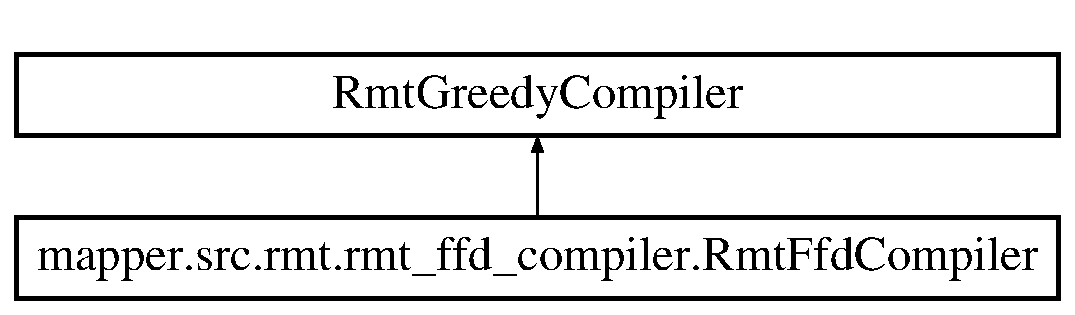
\includegraphics[height=2.000000cm]{classmapper_1_1src_1_1rmt_1_1rmt__ffd__compiler_1_1_rmt_ffd_compiler}
\end{center}
\end{figure}
\subsection*{Public Member Functions}
\begin{DoxyCompactItemize}
\item 
\hypertarget{classmapper_1_1src_1_1rmt_1_1rmt__ffd__compiler_1_1_rmt_ffd_compiler_aebeb9e79e7293b474b85e4fb2327d0b8}{}def {\bfseries \+\_\+\+\_\+init\+\_\+\+\_\+}\label{classmapper_1_1src_1_1rmt_1_1rmt__ffd__compiler_1_1_rmt_ffd_compiler_aebeb9e79e7293b474b85e4fb2327d0b8}

\item 
\hypertarget{classmapper_1_1src_1_1rmt_1_1rmt__ffd__compiler_1_1_rmt_ffd_compiler_ab1f8b004da864c0a71abbbb88a6c2455}{}def {\bfseries get\+Limiting\+Resource\+Use} (self, table)\label{classmapper_1_1src_1_1rmt_1_1rmt__ffd__compiler_1_1_rmt_ffd_compiler_ab1f8b004da864c0a71abbbb88a6c2455}

\item 
def \hyperlink{classmapper_1_1src_1_1rmt_1_1rmt__ffd__compiler_1_1_rmt_ffd_compiler_a72d044d7eb34031daeb42909502c0860}{get\+Ordered\+Tables} (self)
\end{DoxyCompactItemize}
\subsection*{Public Attributes}
\begin{DoxyCompactItemize}
\item 
\hypertarget{classmapper_1_1src_1_1rmt_1_1rmt__ffd__compiler_1_1_rmt_ffd_compiler_a7f40f5f121621d17f98d3b04993ce681}{}{\bfseries logger}\label{classmapper_1_1src_1_1rmt_1_1rmt__ffd__compiler_1_1_rmt_ffd_compiler_a7f40f5f121621d17f98d3b04993ce681}

\item 
\hypertarget{classmapper_1_1src_1_1rmt_1_1rmt__ffd__compiler_1_1_rmt_ffd_compiler_aca6b71ccb30184d0c8fc9904474a9f34}{}{\bfseries ordered\+Tables}\label{classmapper_1_1src_1_1rmt_1_1rmt__ffd__compiler_1_1_rmt_ffd_compiler_aca6b71ccb30184d0c8fc9904474a9f34}

\end{DoxyCompactItemize}


\subsection{Member Function Documentation}
\hypertarget{classmapper_1_1src_1_1rmt_1_1rmt__ffd__compiler_1_1_rmt_ffd_compiler_a72d044d7eb34031daeb42909502c0860}{}\index{mapper\+::src\+::rmt\+::rmt\+\_\+ffd\+\_\+compiler\+::\+Rmt\+Ffd\+Compiler@{mapper\+::src\+::rmt\+::rmt\+\_\+ffd\+\_\+compiler\+::\+Rmt\+Ffd\+Compiler}!get\+Ordered\+Tables@{get\+Ordered\+Tables}}
\index{get\+Ordered\+Tables@{get\+Ordered\+Tables}!mapper\+::src\+::rmt\+::rmt\+\_\+ffd\+\_\+compiler\+::\+Rmt\+Ffd\+Compiler@{mapper\+::src\+::rmt\+::rmt\+\_\+ffd\+\_\+compiler\+::\+Rmt\+Ffd\+Compiler}}
\subsubsection[{get\+Ordered\+Tables(self)}]{\setlength{\rightskip}{0pt plus 5cm}def mapper.\+src.\+rmt.\+rmt\+\_\+ffd\+\_\+compiler.\+Rmt\+Ffd\+Compiler.\+get\+Ordered\+Tables (
\begin{DoxyParamCaption}
\item[{}]{self}
\end{DoxyParamCaption}
)}\label{classmapper_1_1src_1_1rmt_1_1rmt__ffd__compiler_1_1_rmt_ffd_compiler_a72d044d7eb34031daeb42909502c0860}
\begin{DoxyVerb}Return tables in order of limiting resource- if a table needs 2 out 8 available input xbar units
and 512 of say 1024 available bits of the action data xbar (in every stage), then action data xbar
is the limiting resources, since it need 50% of the available resource per stage
(vs 25% for input xbar). \end{DoxyVerb}
 

The documentation for this class was generated from the following file\+:\begin{DoxyCompactItemize}
\item 
src/rmt/rmt\+\_\+ffd\+\_\+compiler.\+py\end{DoxyCompactItemize}

\hypertarget{classmapper_1_1src_1_1rmt_1_1rmt__ffl__compiler_1_1_rmt_ffl_compiler}{}\section{mapper.\+src.\+rmt.\+rmt\+\_\+ffl\+\_\+compiler.\+Rmt\+Ffl\+Compiler Class Reference}
\label{classmapper_1_1src_1_1rmt_1_1rmt__ffl__compiler_1_1_rmt_ffl_compiler}\index{mapper.\+src.\+rmt.\+rmt\+\_\+ffl\+\_\+compiler.\+Rmt\+Ffl\+Compiler@{mapper.\+src.\+rmt.\+rmt\+\_\+ffl\+\_\+compiler.\+Rmt\+Ffl\+Compiler}}
Inheritance diagram for mapper.\+src.\+rmt.\+rmt\+\_\+ffl\+\_\+compiler.\+Rmt\+Ffl\+Compiler\+:\begin{figure}[H]
\begin{center}
\leavevmode
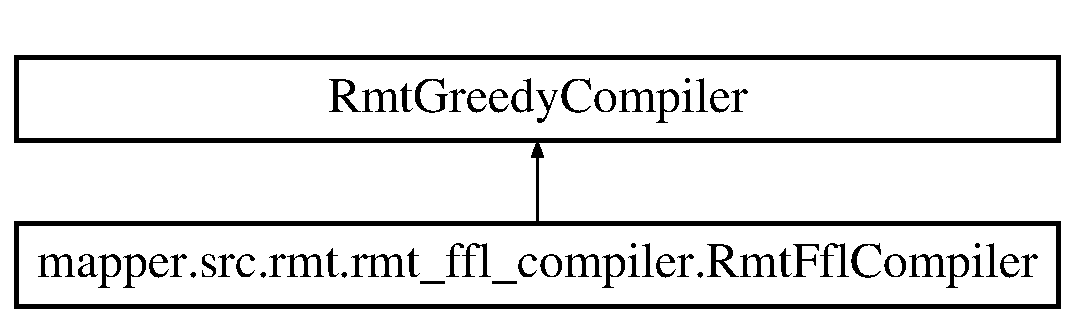
\includegraphics[height=2.000000cm]{classmapper_1_1src_1_1rmt_1_1rmt__ffl__compiler_1_1_rmt_ffl_compiler}
\end{center}
\end{figure}
\subsection*{Public Member Functions}
\begin{DoxyCompactItemize}
\item 
\hypertarget{classmapper_1_1src_1_1rmt_1_1rmt__ffl__compiler_1_1_rmt_ffl_compiler_acc84be0d3963122d881a145c1ee3785f}{}def {\bfseries \+\_\+\+\_\+init\+\_\+\+\_\+}\label{classmapper_1_1src_1_1rmt_1_1rmt__ffl__compiler_1_1_rmt_ffl_compiler_acc84be0d3963122d881a145c1ee3785f}

\item 
def \hyperlink{classmapper_1_1src_1_1rmt_1_1rmt__ffl__compiler_1_1_rmt_ffl_compiler_a8e28a57bf24f9b3fa6fddf2cd130367e}{get\+Ordered\+Tables} (self)
\end{DoxyCompactItemize}
\subsection*{Public Attributes}
\begin{DoxyCompactItemize}
\item 
\hypertarget{classmapper_1_1src_1_1rmt_1_1rmt__ffl__compiler_1_1_rmt_ffl_compiler_a519fa08009da9d1b1d9085774f629acd}{}{\bfseries logger}\label{classmapper_1_1src_1_1rmt_1_1rmt__ffl__compiler_1_1_rmt_ffl_compiler_a519fa08009da9d1b1d9085774f629acd}

\item 
\hypertarget{classmapper_1_1src_1_1rmt_1_1rmt__ffl__compiler_1_1_rmt_ffl_compiler_aa3d98e304d5e0e8a9ee3e133a49da054}{}{\bfseries ordered\+Tables}\label{classmapper_1_1src_1_1rmt_1_1rmt__ffl__compiler_1_1_rmt_ffl_compiler_aa3d98e304d5e0e8a9ee3e133a49da054}

\end{DoxyCompactItemize}


\subsection{Member Function Documentation}
\hypertarget{classmapper_1_1src_1_1rmt_1_1rmt__ffl__compiler_1_1_rmt_ffl_compiler_a8e28a57bf24f9b3fa6fddf2cd130367e}{}\index{mapper\+::src\+::rmt\+::rmt\+\_\+ffl\+\_\+compiler\+::\+Rmt\+Ffl\+Compiler@{mapper\+::src\+::rmt\+::rmt\+\_\+ffl\+\_\+compiler\+::\+Rmt\+Ffl\+Compiler}!get\+Ordered\+Tables@{get\+Ordered\+Tables}}
\index{get\+Ordered\+Tables@{get\+Ordered\+Tables}!mapper\+::src\+::rmt\+::rmt\+\_\+ffl\+\_\+compiler\+::\+Rmt\+Ffl\+Compiler@{mapper\+::src\+::rmt\+::rmt\+\_\+ffl\+\_\+compiler\+::\+Rmt\+Ffl\+Compiler}}
\subsubsection[{get\+Ordered\+Tables(self)}]{\setlength{\rightskip}{0pt plus 5cm}def mapper.\+src.\+rmt.\+rmt\+\_\+ffl\+\_\+compiler.\+Rmt\+Ffl\+Compiler.\+get\+Ordered\+Tables (
\begin{DoxyParamCaption}
\item[{}]{self}
\end{DoxyParamCaption}
)}\label{classmapper_1_1src_1_1rmt_1_1rmt__ffl__compiler_1_1_rmt_ffl_compiler_a8e28a57bf24f9b3fa6fddf2cd130367e}
\begin{DoxyVerb}Return tables in order of level- number of edges in the longest dependency
path to the end of the program, where an edge/ dependency has weight 1 if it forces
the second table to a new stage\end{DoxyVerb}
 

The documentation for this class was generated from the following file\+:\begin{DoxyCompactItemize}
\item 
src/rmt/rmt\+\_\+ffl\+\_\+compiler.\+py\end{DoxyCompactItemize}

\hypertarget{classmapper_1_1src_1_1rmt_1_1rmt__ffls__compiler_1_1_rmt_ffls_compiler}{}\section{mapper.\+src.\+rmt.\+rmt\+\_\+ffls\+\_\+compiler.\+Rmt\+Ffls\+Compiler Class Reference}
\label{classmapper_1_1src_1_1rmt_1_1rmt__ffls__compiler_1_1_rmt_ffls_compiler}\index{mapper.\+src.\+rmt.\+rmt\+\_\+ffls\+\_\+compiler.\+Rmt\+Ffls\+Compiler@{mapper.\+src.\+rmt.\+rmt\+\_\+ffls\+\_\+compiler.\+Rmt\+Ffls\+Compiler}}
Inheritance diagram for mapper.\+src.\+rmt.\+rmt\+\_\+ffls\+\_\+compiler.\+Rmt\+Ffls\+Compiler\+:\begin{figure}[H]
\begin{center}
\leavevmode
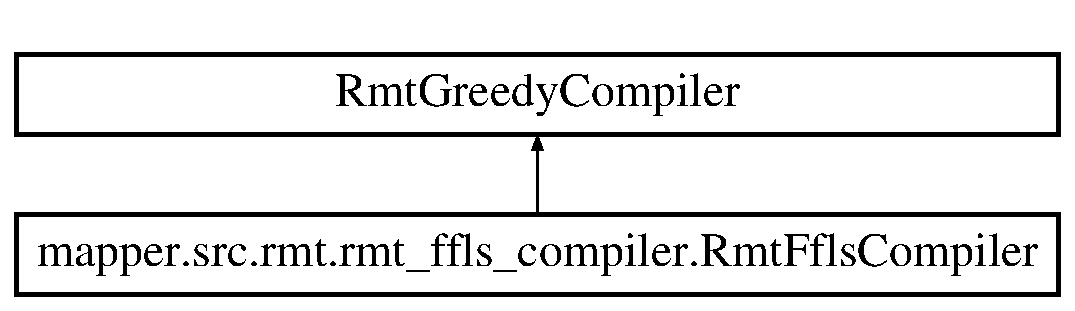
\includegraphics[height=2.000000cm]{classmapper_1_1src_1_1rmt_1_1rmt__ffls__compiler_1_1_rmt_ffls_compiler}
\end{center}
\end{figure}
\subsection*{Public Member Functions}
\begin{DoxyCompactItemize}
\item 
\hypertarget{classmapper_1_1src_1_1rmt_1_1rmt__ffls__compiler_1_1_rmt_ffls_compiler_a5aebcf00c693946f8b52bf70e297d556}{}def {\bfseries \+\_\+\+\_\+init\+\_\+\+\_\+}\label{classmapper_1_1src_1_1rmt_1_1rmt__ffls__compiler_1_1_rmt_ffls_compiler_a5aebcf00c693946f8b52bf70e297d556}

\item 
\hypertarget{classmapper_1_1src_1_1rmt_1_1rmt__ffls__compiler_1_1_rmt_ffls_compiler_aa6f9e784da825b5920eb57a615a7e30d}{}def {\bfseries get\+Num\+Stages} (self, table\+Index)\label{classmapper_1_1src_1_1rmt_1_1rmt__ffls__compiler_1_1_rmt_ffls_compiler_aa6f9e784da825b5920eb57a615a7e30d}

\item 
\hypertarget{classmapper_1_1src_1_1rmt_1_1rmt__ffls__compiler_1_1_rmt_ffls_compiler_a88ac523960acfcb462fb4ceaa242516c}{}def {\bfseries get\+Ordered\+Tables} (self)\label{classmapper_1_1src_1_1rmt_1_1rmt__ffls__compiler_1_1_rmt_ffls_compiler_a88ac523960acfcb462fb4ceaa242516c}

\end{DoxyCompactItemize}
\subsection*{Public Attributes}
\begin{DoxyCompactItemize}
\item 
\hypertarget{classmapper_1_1src_1_1rmt_1_1rmt__ffls__compiler_1_1_rmt_ffls_compiler_aa476dbdb3befc113eb21a56ba610f574}{}{\bfseries logger}\label{classmapper_1_1src_1_1rmt_1_1rmt__ffls__compiler_1_1_rmt_ffls_compiler_aa476dbdb3befc113eb21a56ba610f574}

\item 
\hypertarget{classmapper_1_1src_1_1rmt_1_1rmt__ffls__compiler_1_1_rmt_ffls_compiler_a222827abed9da46969d45d4a9cd76e04}{}{\bfseries ordered\+Tables}\label{classmapper_1_1src_1_1rmt_1_1rmt__ffls__compiler_1_1_rmt_ffls_compiler_a222827abed9da46969d45d4a9cd76e04}

\end{DoxyCompactItemize}


The documentation for this class was generated from the following file\+:\begin{DoxyCompactItemize}
\item 
src/rmt/rmt\+\_\+ffls\+\_\+compiler.\+py\end{DoxyCompactItemize}

\hypertarget{classmapper_1_1src_1_1rmt_1_1rmt__greedy__compiler_1_1_rmt_greedy_compiler}{}\section{mapper.\+src.\+rmt.\+rmt\+\_\+greedy\+\_\+compiler.\+Rmt\+Greedy\+Compiler Class Reference}
\label{classmapper_1_1src_1_1rmt_1_1rmt__greedy__compiler_1_1_rmt_greedy_compiler}\index{mapper.\+src.\+rmt.\+rmt\+\_\+greedy\+\_\+compiler.\+Rmt\+Greedy\+Compiler@{mapper.\+src.\+rmt.\+rmt\+\_\+greedy\+\_\+compiler.\+Rmt\+Greedy\+Compiler}}
\subsection*{Public Member Functions}
\begin{DoxyCompactItemize}
\item 
\hypertarget{classmapper_1_1src_1_1rmt_1_1rmt__greedy__compiler_1_1_rmt_greedy_compiler_a4ec3e834ee75df91095a330477806cd0}{}def {\bfseries \+\_\+\+\_\+init\+\_\+\+\_\+}\label{classmapper_1_1src_1_1rmt_1_1rmt__greedy__compiler_1_1_rmt_greedy_compiler_a4ec3e834ee75df91095a330477806cd0}

\item 
def \hyperlink{classmapper_1_1src_1_1rmt_1_1rmt__greedy__compiler_1_1_rmt_greedy_compiler_aeb2db53582c9e835a96af87fb6ecadd4}{get\+Index} (self, table, names)
\item 
def \hyperlink{classmapper_1_1src_1_1rmt_1_1rmt__greedy__compiler_1_1_rmt_greedy_compiler_a07cf4ee1907b1f1d65b50ae2a0df7485}{get\+Best\+Fit\+For\+Words} (self, table\+Index, mem, last\+Block, num\+Words\+Left)
\item 
def \hyperlink{classmapper_1_1src_1_1rmt_1_1rmt__greedy__compiler_1_1_rmt_greedy_compiler_a5eadae139fff0060c66714bc05f57e02}{get\+Per\+Pf} (self, mem, table\+Index)
\item 
def \hyperlink{classmapper_1_1src_1_1rmt_1_1rmt__greedy__compiler_1_1_rmt_greedy_compiler_a34b2e3bb99ee2426b356194f882c177f}{get\+Best\+Fit\+For\+Blocks} (self, table\+Index, mem, last\+Block, num\+Sram\+Blocks\+Reserved)
\item 
def \hyperlink{classmapper_1_1src_1_1rmt_1_1rmt__greedy__compiler_1_1_rmt_greedy_compiler_a38079b7112774a71291c150d4f8b9a42}{get\+Next\+Table} (self)
\item 
\hypertarget{classmapper_1_1src_1_1rmt_1_1rmt__greedy__compiler_1_1_rmt_greedy_compiler_a45fcf1c9b9707e3a6c21ce4ec078f256}{}def {\bfseries get\+Mem} (self, table\+Index)\label{classmapper_1_1src_1_1rmt_1_1rmt__greedy__compiler_1_1_rmt_greedy_compiler_a45fcf1c9b9707e3a6c21ce4ec078f256}

\item 
\hypertarget{classmapper_1_1src_1_1rmt_1_1rmt__greedy__compiler_1_1_rmt_greedy_compiler_ac7a09cd6bfedf947a3cdf9af51d121ef}{}def {\bfseries get\+Input\+Crossbar\+Subunits} (self, table\+Index, mem)\label{classmapper_1_1src_1_1rmt_1_1rmt__greedy__compiler_1_1_rmt_greedy_compiler_ac7a09cd6bfedf947a3cdf9af51d121ef}

\item 
\hypertarget{classmapper_1_1src_1_1rmt_1_1rmt__greedy__compiler_1_1_rmt_greedy_compiler_a261d7c534eb127acc847abea885b79ab}{}def {\bfseries get\+Maximum\+Input\+Crossbar\+Subunits} (self, table\+Index, mem)\label{classmapper_1_1src_1_1rmt_1_1rmt__greedy__compiler_1_1_rmt_greedy_compiler_a261d7c534eb127acc847abea885b79ab}

\item 
\hypertarget{classmapper_1_1src_1_1rmt_1_1rmt__greedy__compiler_1_1_rmt_greedy_compiler_ad420355b358ca5473a3b3ec2977da043}{}def {\bfseries get\+Available\+Input\+Crossbar\+Subunits} (self, table\+Index, mem)\label{classmapper_1_1src_1_1rmt_1_1rmt__greedy__compiler_1_1_rmt_greedy_compiler_ad420355b358ca5473a3b3ec2977da043}

\item 
\hypertarget{classmapper_1_1src_1_1rmt_1_1rmt__greedy__compiler_1_1_rmt_greedy_compiler_afc19b2bff59e896ca57b92520244e3c3}{}def {\bfseries get\+Width\+Action\+Data} (self, table\+Index)\label{classmapper_1_1src_1_1rmt_1_1rmt__greedy__compiler_1_1_rmt_greedy_compiler_afc19b2bff59e896ca57b92520244e3c3}

\item 
\hypertarget{classmapper_1_1src_1_1rmt_1_1rmt__greedy__compiler_1_1_rmt_greedy_compiler_a363dfb0cadbdb5761822069e5785c0bd}{}def {\bfseries get\+Maximum\+Width\+Action\+Data} (self, table\+Index, mem)\label{classmapper_1_1src_1_1rmt_1_1rmt__greedy__compiler_1_1_rmt_greedy_compiler_a363dfb0cadbdb5761822069e5785c0bd}

\item 
\hypertarget{classmapper_1_1src_1_1rmt_1_1rmt__greedy__compiler_1_1_rmt_greedy_compiler_a790298e116411b88ecb23b61580f6ac0}{}def {\bfseries get\+Available\+Width\+Action\+Data} (self, table\+Index, mem)\label{classmapper_1_1src_1_1rmt_1_1rmt__greedy__compiler_1_1_rmt_greedy_compiler_a790298e116411b88ecb23b61580f6ac0}

\item 
\hypertarget{classmapper_1_1src_1_1rmt_1_1rmt__greedy__compiler_1_1_rmt_greedy_compiler_ae6d651b30ce268196c75c83984fabb84}{}def {\bfseries update\+Last\+Block\+And\+Assign}\label{classmapper_1_1src_1_1rmt_1_1rmt__greedy__compiler_1_1_rmt_greedy_compiler_ae6d651b30ce268196c75c83984fabb84}

\item 
def \hyperlink{classmapper_1_1src_1_1rmt_1_1rmt__greedy__compiler_1_1_rmt_greedy_compiler_a7dd783a7aceecadc6751d219a9f7b12c}{get\+Num\+Sram\+Blocks\+Reserved} (self)
\item 
\hypertarget{classmapper_1_1src_1_1rmt_1_1rmt__greedy__compiler_1_1_rmt_greedy_compiler_adfe208d6e4bfa1269cdc06d3d45a72c2}{}def {\bfseries log\+Compiler\+Attempt} (self, compiler\+Attempt)\label{classmapper_1_1src_1_1rmt_1_1rmt__greedy__compiler_1_1_rmt_greedy_compiler_adfe208d6e4bfa1269cdc06d3d45a72c2}

\item 
def \hyperlink{classmapper_1_1src_1_1rmt_1_1rmt__greedy__compiler_1_1_rmt_greedy_compiler_a4ffb6d0ee0b2fe3a87da2177d5981243}{solve} (self, program, switch, preprocess)
\end{DoxyCompactItemize}
\subsection*{Public Attributes}
\begin{DoxyCompactItemize}
\item 
\hypertarget{classmapper_1_1src_1_1rmt_1_1rmt__greedy__compiler_1_1_rmt_greedy_compiler_a1287ca0951538e9a52ff483f845f2b01}{}{\bfseries num\+Sram\+Blocks\+Reserved}\label{classmapper_1_1src_1_1rmt_1_1rmt__greedy__compiler_1_1_rmt_greedy_compiler_a1287ca0951538e9a52ff483f845f2b01}

\item 
\hypertarget{classmapper_1_1src_1_1rmt_1_1rmt__greedy__compiler_1_1_rmt_greedy_compiler_a30bd8d1a9082c244044d59e2107a3d34}{}{\bfseries version}\label{classmapper_1_1src_1_1rmt_1_1rmt__greedy__compiler_1_1_rmt_greedy_compiler_a30bd8d1a9082c244044d59e2107a3d34}

\item 
\hypertarget{classmapper_1_1src_1_1rmt_1_1rmt__greedy__compiler_1_1_rmt_greedy_compiler_ab65399f022e4177fbd19de3d93478c39}{}{\bfseries logger}\label{classmapper_1_1src_1_1rmt_1_1rmt__greedy__compiler_1_1_rmt_greedy_compiler_ab65399f022e4177fbd19de3d93478c39}

\item 
\hypertarget{classmapper_1_1src_1_1rmt_1_1rmt__greedy__compiler_1_1_rmt_greedy_compiler_a14427ce44c572c5f4402930d0a91213f}{}{\bfseries program}\label{classmapper_1_1src_1_1rmt_1_1rmt__greedy__compiler_1_1_rmt_greedy_compiler_a14427ce44c572c5f4402930d0a91213f}

\item 
\hypertarget{classmapper_1_1src_1_1rmt_1_1rmt__greedy__compiler_1_1_rmt_greedy_compiler_a3eee88963b342610e8f5d5fb43926c82}{}{\bfseries switch}\label{classmapper_1_1src_1_1rmt_1_1rmt__greedy__compiler_1_1_rmt_greedy_compiler_a3eee88963b342610e8f5d5fb43926c82}

\item 
\hypertarget{classmapper_1_1src_1_1rmt_1_1rmt__greedy__compiler_1_1_rmt_greedy_compiler_aaba9dc5f849b7e4f4709f297744d8fe4}{}{\bfseries preprocess}\label{classmapper_1_1src_1_1rmt_1_1rmt__greedy__compiler_1_1_rmt_greedy_compiler_aaba9dc5f849b7e4f4709f297744d8fe4}

\item 
\hypertarget{classmapper_1_1src_1_1rmt_1_1rmt__greedy__compiler_1_1_rmt_greedy_compiler_a593dbfd0f94456f57569073c8682ff07}{}{\bfseries results}\label{classmapper_1_1src_1_1rmt_1_1rmt__greedy__compiler_1_1_rmt_greedy_compiler_a593dbfd0f94456f57569073c8682ff07}

\item 
\hypertarget{classmapper_1_1src_1_1rmt_1_1rmt__greedy__compiler_1_1_rmt_greedy_compiler_aebd8df3db5814dc137a3583b9f211027}{}{\bfseries gr}\label{classmapper_1_1src_1_1rmt_1_1rmt__greedy__compiler_1_1_rmt_greedy_compiler_aebd8df3db5814dc137a3583b9f211027}

\item 
\hypertarget{classmapper_1_1src_1_1rmt_1_1rmt__greedy__compiler_1_1_rmt_greedy_compiler_a2bb63b1587729b9589357dd7676a55b5}{}{\bfseries blocks\+Per\+St}\label{classmapper_1_1src_1_1rmt_1_1rmt__greedy__compiler_1_1_rmt_greedy_compiler_a2bb63b1587729b9589357dd7676a55b5}

\item 
\hypertarget{classmapper_1_1src_1_1rmt_1_1rmt__greedy__compiler_1_1_rmt_greedy_compiler_abe67939a02beb235e20c7974184e54a9}{}{\bfseries num\+Blocks}\label{classmapper_1_1src_1_1rmt_1_1rmt__greedy__compiler_1_1_rmt_greedy_compiler_abe67939a02beb235e20c7974184e54a9}

\item 
\hypertarget{classmapper_1_1src_1_1rmt_1_1rmt__greedy__compiler_1_1_rmt_greedy_compiler_a94dbe5a475163e557474f9faf21e8df3}{}{\bfseries blocks\+Per\+Pf}\label{classmapper_1_1src_1_1rmt_1_1rmt__greedy__compiler_1_1_rmt_greedy_compiler_a94dbe5a475163e557474f9faf21e8df3}

\item 
\hypertarget{classmapper_1_1src_1_1rmt_1_1rmt__greedy__compiler_1_1_rmt_greedy_compiler_a4459846368d21c91cfea0cf9d0f08022}{}{\bfseries words\+Per\+Pf}\label{classmapper_1_1src_1_1rmt_1_1rmt__greedy__compiler_1_1_rmt_greedy_compiler_a4459846368d21c91cfea0cf9d0f08022}

\item 
\hypertarget{classmapper_1_1src_1_1rmt_1_1rmt__greedy__compiler_1_1_rmt_greedy_compiler_a054683283273844734defa24d8159cfe}{}{\bfseries layout}\label{classmapper_1_1src_1_1rmt_1_1rmt__greedy__compiler_1_1_rmt_greedy_compiler_a054683283273844734defa24d8159cfe}

\item 
\hypertarget{classmapper_1_1src_1_1rmt_1_1rmt__greedy__compiler_1_1_rmt_greedy_compiler_adb6864a0a7ac9320b35b42c97582b345}{}{\bfseries block}\label{classmapper_1_1src_1_1rmt_1_1rmt__greedy__compiler_1_1_rmt_greedy_compiler_adb6864a0a7ac9320b35b42c97582b345}

\item 
\hypertarget{classmapper_1_1src_1_1rmt_1_1rmt__greedy__compiler_1_1_rmt_greedy_compiler_aa8c63221d26dff4f552a391c16c316b4}{}{\bfseries word}\label{classmapper_1_1src_1_1rmt_1_1rmt__greedy__compiler_1_1_rmt_greedy_compiler_aa8c63221d26dff4f552a391c16c316b4}

\item 
\hypertarget{classmapper_1_1src_1_1rmt_1_1rmt__greedy__compiler_1_1_rmt_greedy_compiler_a32c678217db3abc6899fc067a6d006db}{}{\bfseries input\+Crossbar}\label{classmapper_1_1src_1_1rmt_1_1rmt__greedy__compiler_1_1_rmt_greedy_compiler_a32c678217db3abc6899fc067a6d006db}

\item 
\hypertarget{classmapper_1_1src_1_1rmt_1_1rmt__greedy__compiler_1_1_rmt_greedy_compiler_a59fb735789a87da78836b732dd571ee8}{}{\bfseries action\+Crossbar}\label{classmapper_1_1src_1_1rmt_1_1rmt__greedy__compiler_1_1_rmt_greedy_compiler_a59fb735789a87da78836b732dd571ee8}

\item 
\hypertarget{classmapper_1_1src_1_1rmt_1_1rmt__greedy__compiler_1_1_rmt_greedy_compiler_a5dec757d516786e121913fdfb22249e4}{}{\bfseries last\+Block}\label{classmapper_1_1src_1_1rmt_1_1rmt__greedy__compiler_1_1_rmt_greedy_compiler_a5dec757d516786e121913fdfb22249e4}

\item 
\hypertarget{classmapper_1_1src_1_1rmt_1_1rmt__greedy__compiler_1_1_rmt_greedy_compiler_a562bcd62be31ac69c47300a884e5becf}{}{\bfseries assigned}\label{classmapper_1_1src_1_1rmt_1_1rmt__greedy__compiler_1_1_rmt_greedy_compiler_a562bcd62be31ac69c47300a884e5becf}

\item 
\hypertarget{classmapper_1_1src_1_1rmt_1_1rmt__greedy__compiler_1_1_rmt_greedy_compiler_a2a6cb9f87bcc37b0b127072b348e5cb0}{}{\bfseries current\+Stage}\label{classmapper_1_1src_1_1rmt_1_1rmt__greedy__compiler_1_1_rmt_greedy_compiler_a2a6cb9f87bcc37b0b127072b348e5cb0}

\item 
\hypertarget{classmapper_1_1src_1_1rmt_1_1rmt__greedy__compiler_1_1_rmt_greedy_compiler_a2f9165d45290bcf6a83be15955fba50b}{}{\bfseries table}\label{classmapper_1_1src_1_1rmt_1_1rmt__greedy__compiler_1_1_rmt_greedy_compiler_a2f9165d45290bcf6a83be15955fba50b}

\item 
\hypertarget{classmapper_1_1src_1_1rmt_1_1rmt__greedy__compiler_1_1_rmt_greedy_compiler_afd24d16810706eafc4a9e5e1e9b2d7ee}{}{\bfseries num\+Words\+Left}\label{classmapper_1_1src_1_1rmt_1_1rmt__greedy__compiler_1_1_rmt_greedy_compiler_afd24d16810706eafc4a9e5e1e9b2d7ee}

\end{DoxyCompactItemize}


\subsection{Detailed Description}
\begin{DoxyVerb}Greedy heuristic compiler, the specific greedy heuristic
is determined by the getOrderedTables function defined in
child classes RmtFFlCompiler and RmtFfdCompiler etc.
\end{DoxyVerb}
 

\subsection{Member Function Documentation}
\hypertarget{classmapper_1_1src_1_1rmt_1_1rmt__greedy__compiler_1_1_rmt_greedy_compiler_a34b2e3bb99ee2426b356194f882c177f}{}\index{mapper\+::src\+::rmt\+::rmt\+\_\+greedy\+\_\+compiler\+::\+Rmt\+Greedy\+Compiler@{mapper\+::src\+::rmt\+::rmt\+\_\+greedy\+\_\+compiler\+::\+Rmt\+Greedy\+Compiler}!get\+Best\+Fit\+For\+Blocks@{get\+Best\+Fit\+For\+Blocks}}
\index{get\+Best\+Fit\+For\+Blocks@{get\+Best\+Fit\+For\+Blocks}!mapper\+::src\+::rmt\+::rmt\+\_\+greedy\+\_\+compiler\+::\+Rmt\+Greedy\+Compiler@{mapper\+::src\+::rmt\+::rmt\+\_\+greedy\+\_\+compiler\+::\+Rmt\+Greedy\+Compiler}}
\subsubsection[{get\+Best\+Fit\+For\+Blocks(self, table\+Index, mem, last\+Block, num\+Sram\+Blocks\+Reserved)}]{\setlength{\rightskip}{0pt plus 5cm}def mapper.\+src.\+rmt.\+rmt\+\_\+greedy\+\_\+compiler.\+Rmt\+Greedy\+Compiler.\+get\+Best\+Fit\+For\+Blocks (
\begin{DoxyParamCaption}
\item[{}]{self, }
\item[{}]{table\+Index, }
\item[{}]{mem, }
\item[{}]{last\+Block, }
\item[{}]{num\+Sram\+Blocks\+Reserved}
\end{DoxyParamCaption}
)}\label{classmapper_1_1src_1_1rmt_1_1rmt__greedy__compiler_1_1_rmt_greedy_compiler_a34b2e3bb99ee2426b356194f882c177f}
\begin{DoxyVerb}Given number of blocks available, find a config. (i.e., pick a
packing unit) to fit the maximum number of entries possible
Based solely on memory resources needed for match and action data,
not other resources like crossbar units etc.
\end{DoxyVerb}
 \hypertarget{classmapper_1_1src_1_1rmt_1_1rmt__greedy__compiler_1_1_rmt_greedy_compiler_a07cf4ee1907b1f1d65b50ae2a0df7485}{}\index{mapper\+::src\+::rmt\+::rmt\+\_\+greedy\+\_\+compiler\+::\+Rmt\+Greedy\+Compiler@{mapper\+::src\+::rmt\+::rmt\+\_\+greedy\+\_\+compiler\+::\+Rmt\+Greedy\+Compiler}!get\+Best\+Fit\+For\+Words@{get\+Best\+Fit\+For\+Words}}
\index{get\+Best\+Fit\+For\+Words@{get\+Best\+Fit\+For\+Words}!mapper\+::src\+::rmt\+::rmt\+\_\+greedy\+\_\+compiler\+::\+Rmt\+Greedy\+Compiler@{mapper\+::src\+::rmt\+::rmt\+\_\+greedy\+\_\+compiler\+::\+Rmt\+Greedy\+Compiler}}
\subsubsection[{get\+Best\+Fit\+For\+Words(self, table\+Index, mem, last\+Block, num\+Words\+Left)}]{\setlength{\rightskip}{0pt plus 5cm}def mapper.\+src.\+rmt.\+rmt\+\_\+greedy\+\_\+compiler.\+Rmt\+Greedy\+Compiler.\+get\+Best\+Fit\+For\+Words (
\begin{DoxyParamCaption}
\item[{}]{self, }
\item[{}]{table\+Index, }
\item[{}]{mem, }
\item[{}]{last\+Block, }
\item[{}]{num\+Words\+Left}
\end{DoxyParamCaption}
)}\label{classmapper_1_1src_1_1rmt_1_1rmt__greedy__compiler_1_1_rmt_greedy_compiler_a07cf4ee1907b1f1d65b50ae2a0df7485}
\begin{DoxyVerb}Given the number of match entries left, find minimum number of
blocks needed to fit all of them
Based solely on memory resources needed for match and action data,
not other resources like crossbar units etc.
\end{DoxyVerb}
 \hypertarget{classmapper_1_1src_1_1rmt_1_1rmt__greedy__compiler_1_1_rmt_greedy_compiler_aeb2db53582c9e835a96af87fb6ecadd4}{}\index{mapper\+::src\+::rmt\+::rmt\+\_\+greedy\+\_\+compiler\+::\+Rmt\+Greedy\+Compiler@{mapper\+::src\+::rmt\+::rmt\+\_\+greedy\+\_\+compiler\+::\+Rmt\+Greedy\+Compiler}!get\+Index@{get\+Index}}
\index{get\+Index@{get\+Index}!mapper\+::src\+::rmt\+::rmt\+\_\+greedy\+\_\+compiler\+::\+Rmt\+Greedy\+Compiler@{mapper\+::src\+::rmt\+::rmt\+\_\+greedy\+\_\+compiler\+::\+Rmt\+Greedy\+Compiler}}
\subsubsection[{get\+Index(self, table, names)}]{\setlength{\rightskip}{0pt plus 5cm}def mapper.\+src.\+rmt.\+rmt\+\_\+greedy\+\_\+compiler.\+Rmt\+Greedy\+Compiler.\+get\+Index (
\begin{DoxyParamCaption}
\item[{}]{self, }
\item[{}]{table, }
\item[{}]{names}
\end{DoxyParamCaption}
)}\label{classmapper_1_1src_1_1rmt_1_1rmt__greedy__compiler_1_1_rmt_greedy_compiler_aeb2db53582c9e835a96af87fb6ecadd4}
\begin{DoxyVerb}Returns index of table in names\end{DoxyVerb}
 \hypertarget{classmapper_1_1src_1_1rmt_1_1rmt__greedy__compiler_1_1_rmt_greedy_compiler_a38079b7112774a71291c150d4f8b9a42}{}\index{mapper\+::src\+::rmt\+::rmt\+\_\+greedy\+\_\+compiler\+::\+Rmt\+Greedy\+Compiler@{mapper\+::src\+::rmt\+::rmt\+\_\+greedy\+\_\+compiler\+::\+Rmt\+Greedy\+Compiler}!get\+Next\+Table@{get\+Next\+Table}}
\index{get\+Next\+Table@{get\+Next\+Table}!mapper\+::src\+::rmt\+::rmt\+\_\+greedy\+\_\+compiler\+::\+Rmt\+Greedy\+Compiler@{mapper\+::src\+::rmt\+::rmt\+\_\+greedy\+\_\+compiler\+::\+Rmt\+Greedy\+Compiler}}
\subsubsection[{get\+Next\+Table(self)}]{\setlength{\rightskip}{0pt plus 5cm}def mapper.\+src.\+rmt.\+rmt\+\_\+greedy\+\_\+compiler.\+Rmt\+Greedy\+Compiler.\+get\+Next\+Table (
\begin{DoxyParamCaption}
\item[{}]{self}
\end{DoxyParamCaption}
)}\label{classmapper_1_1src_1_1rmt_1_1rmt__greedy__compiler_1_1_rmt_greedy_compiler_a38079b7112774a71291c150d4f8b9a42}
\begin{DoxyVerb}Get the next table from the heuristic order that hasn't been
assigned yet.
\end{DoxyVerb}
 \hypertarget{classmapper_1_1src_1_1rmt_1_1rmt__greedy__compiler_1_1_rmt_greedy_compiler_a7dd783a7aceecadc6751d219a9f7b12c}{}\index{mapper\+::src\+::rmt\+::rmt\+\_\+greedy\+\_\+compiler\+::\+Rmt\+Greedy\+Compiler@{mapper\+::src\+::rmt\+::rmt\+\_\+greedy\+\_\+compiler\+::\+Rmt\+Greedy\+Compiler}!get\+Num\+Sram\+Blocks\+Reserved@{get\+Num\+Sram\+Blocks\+Reserved}}
\index{get\+Num\+Sram\+Blocks\+Reserved@{get\+Num\+Sram\+Blocks\+Reserved}!mapper\+::src\+::rmt\+::rmt\+\_\+greedy\+\_\+compiler\+::\+Rmt\+Greedy\+Compiler@{mapper\+::src\+::rmt\+::rmt\+\_\+greedy\+\_\+compiler\+::\+Rmt\+Greedy\+Compiler}}
\subsubsection[{get\+Num\+Sram\+Blocks\+Reserved(self)}]{\setlength{\rightskip}{0pt plus 5cm}def mapper.\+src.\+rmt.\+rmt\+\_\+greedy\+\_\+compiler.\+Rmt\+Greedy\+Compiler.\+get\+Num\+Sram\+Blocks\+Reserved (
\begin{DoxyParamCaption}
\item[{}]{self}
\end{DoxyParamCaption}
)}\label{classmapper_1_1src_1_1rmt_1_1rmt__greedy__compiler_1_1_rmt_greedy_compiler_a7dd783a7aceecadc6751d219a9f7b12c}
\begin{DoxyVerb}Returns number SRAM blocks reserved for the action data of tables
that will go in TCAM
\end{DoxyVerb}
 \hypertarget{classmapper_1_1src_1_1rmt_1_1rmt__greedy__compiler_1_1_rmt_greedy_compiler_a5eadae139fff0060c66714bc05f57e02}{}\index{mapper\+::src\+::rmt\+::rmt\+\_\+greedy\+\_\+compiler\+::\+Rmt\+Greedy\+Compiler@{mapper\+::src\+::rmt\+::rmt\+\_\+greedy\+\_\+compiler\+::\+Rmt\+Greedy\+Compiler}!get\+Per\+Pf@{get\+Per\+Pf}}
\index{get\+Per\+Pf@{get\+Per\+Pf}!mapper\+::src\+::rmt\+::rmt\+\_\+greedy\+\_\+compiler\+::\+Rmt\+Greedy\+Compiler@{mapper\+::src\+::rmt\+::rmt\+\_\+greedy\+\_\+compiler\+::\+Rmt\+Greedy\+Compiler}}
\subsubsection[{get\+Per\+Pf(self, mem, table\+Index)}]{\setlength{\rightskip}{0pt plus 5cm}def mapper.\+src.\+rmt.\+rmt\+\_\+greedy\+\_\+compiler.\+Rmt\+Greedy\+Compiler.\+get\+Per\+Pf (
\begin{DoxyParamCaption}
\item[{}]{self, }
\item[{}]{mem, }
\item[{}]{table\+Index}
\end{DoxyParamCaption}
)}\label{classmapper_1_1src_1_1rmt_1_1rmt__greedy__compiler_1_1_rmt_greedy_compiler_a5eadae139fff0060c66714bc05f57e02}
\begin{DoxyVerb}Get packing unit configurations for given table in given memory type.
\end{DoxyVerb}
 \hypertarget{classmapper_1_1src_1_1rmt_1_1rmt__greedy__compiler_1_1_rmt_greedy_compiler_a4ffb6d0ee0b2fe3a87da2177d5981243}{}\index{mapper\+::src\+::rmt\+::rmt\+\_\+greedy\+\_\+compiler\+::\+Rmt\+Greedy\+Compiler@{mapper\+::src\+::rmt\+::rmt\+\_\+greedy\+\_\+compiler\+::\+Rmt\+Greedy\+Compiler}!solve@{solve}}
\index{solve@{solve}!mapper\+::src\+::rmt\+::rmt\+\_\+greedy\+\_\+compiler\+::\+Rmt\+Greedy\+Compiler@{mapper\+::src\+::rmt\+::rmt\+\_\+greedy\+\_\+compiler\+::\+Rmt\+Greedy\+Compiler}}
\subsubsection[{solve(self, program, switch, preprocess)}]{\setlength{\rightskip}{0pt plus 5cm}def mapper.\+src.\+rmt.\+rmt\+\_\+greedy\+\_\+compiler.\+Rmt\+Greedy\+Compiler.\+solve (
\begin{DoxyParamCaption}
\item[{}]{self, }
\item[{}]{program, }
\item[{}]{switch, }
\item[{}]{preprocess}
\end{DoxyParamCaption}
)}\label{classmapper_1_1src_1_1rmt_1_1rmt__greedy__compiler_1_1_rmt_greedy_compiler_a4ffb6d0ee0b2fe3a87da2177d5981243}
\begin{DoxyVerb}Runs a greedy heuristic and returns switch configuration\end{DoxyVerb}
 

The documentation for this class was generated from the following file\+:\begin{DoxyCompactItemize}
\item 
src/rmt/rmt\+\_\+greedy\+\_\+compiler.\+py\end{DoxyCompactItemize}

\hypertarget{classmapper_1_1src_1_1rmt_1_1orig__rmt__compiler_1_1_rmt_ilp_compiler}{}\section{mapper.\+src.\+rmt.\+orig\+\_\+rmt\+\_\+compiler.\+Rmt\+Ilp\+Compiler Class Reference}
\label{classmapper_1_1src_1_1rmt_1_1orig__rmt__compiler_1_1_rmt_ilp_compiler}\index{mapper.\+src.\+rmt.\+orig\+\_\+rmt\+\_\+compiler.\+Rmt\+Ilp\+Compiler@{mapper.\+src.\+rmt.\+orig\+\_\+rmt\+\_\+compiler.\+Rmt\+Ilp\+Compiler}}
\subsection*{Public Member Functions}
\begin{DoxyCompactItemize}
\item 
def \hyperlink{classmapper_1_1src_1_1rmt_1_1orig__rmt__compiler_1_1_rmt_ilp_compiler_af84883e69fc6fb64376308b9c0879ae1}{\+\_\+\+\_\+init\+\_\+\+\_\+}
\item 
\hypertarget{classmapper_1_1src_1_1rmt_1_1orig__rmt__compiler_1_1_rmt_ilp_compiler_a800d796d8d5f887987c5086f818497dc}{}def {\bfseries set\+Dimension\+Sizes} (self)\label{classmapper_1_1src_1_1rmt_1_1orig__rmt__compiler_1_1_rmt_ilp_compiler_a800d796d8d5f887987c5086f818497dc}

\item 
\hypertarget{classmapper_1_1src_1_1rmt_1_1orig__rmt__compiler_1_1_rmt_ilp_compiler_a36f6c5f3189278265ef055a0da66d20c}{}def {\bfseries compute\+Sum} (self, dict\+Count)\label{classmapper_1_1src_1_1rmt_1_1orig__rmt__compiler_1_1_rmt_ilp_compiler_a36f6c5f3189278265ef055a0da66d20c}

\item 
\hypertarget{classmapper_1_1src_1_1rmt_1_1orig__rmt__compiler_1_1_rmt_ilp_compiler_a8cda2c3c5bc07b5e83faf75f0b26071b}{}def {\bfseries P} (self, l, m)\label{classmapper_1_1src_1_1rmt_1_1orig__rmt__compiler_1_1_rmt_ilp_compiler_a8cda2c3c5bc07b5e83faf75f0b26071b}

\item 
def \hyperlink{classmapper_1_1src_1_1rmt_1_1orig__rmt__compiler_1_1_rmt_ilp_compiler_ace17731f6ed25fbda40a37f78b777d9f}{action\+Assignment\+Constraint} (self)
\item 
def \hyperlink{classmapper_1_1src_1_1rmt_1_1orig__rmt__compiler_1_1_rmt_ilp_compiler_a4eff57998a57301f5ad22b36d5f142a0}{capacity\+Constraint} (self)
\item 
def \hyperlink{classmapper_1_1src_1_1rmt_1_1orig__rmt__compiler_1_1_rmt_ilp_compiler_a665f12ca05865726ea920a1e22ac2f0c}{word\+Layout\+Constraint} (self)
\item 
def \hyperlink{classmapper_1_1src_1_1rmt_1_1orig__rmt__compiler_1_1_rmt_ilp_compiler_a78dbcddce66838280af30531127d0ebb}{use\+Memory\+Constraint} (self)
\item 
def \hyperlink{classmapper_1_1src_1_1rmt_1_1orig__rmt__compiler_1_1_rmt_ilp_compiler_a7590e41d99becfcbe593d490849e5c27}{assignment\+Constraint} (self)
\item 
def \hyperlink{classmapper_1_1src_1_1rmt_1_1orig__rmt__compiler_1_1_rmt_ilp_compiler_a9b9a1d7a64c2dcf0b9cad5f3b814072e}{pipeline\+Latency\+Variables} (self)
\item 
def \hyperlink{classmapper_1_1src_1_1rmt_1_1orig__rmt__compiler_1_1_rmt_ilp_compiler_a2a691d0bb9f0a39959c61e091bf2f518}{get\+Start\+All\+Mem\+Times\+Start\+Time\+Of\+Stage} (self)
\item 
def \hyperlink{classmapper_1_1src_1_1rmt_1_1orig__rmt__compiler_1_1_rmt_ilp_compiler_a5fbfdd61d8b07a0c20de62423f8afd1f}{get\+End\+All\+Mem\+Times\+Start\+Time\+Of\+Stage} (self)
\item 
\hypertarget{classmapper_1_1src_1_1rmt_1_1orig__rmt__compiler_1_1_rmt_ilp_compiler_afc18996a69e909751bd650adfccfb5d0}{}def {\bfseries check\+Pipeline\+Latency\+Constraint} (self, model)\label{classmapper_1_1src_1_1rmt_1_1orig__rmt__compiler_1_1_rmt_ilp_compiler_afc18996a69e909751bd650adfccfb5d0}

\item 
\hypertarget{classmapper_1_1src_1_1rmt_1_1orig__rmt__compiler_1_1_rmt_ilp_compiler_aa3ecc8a7de02a56e076320868bd02291}{}def {\bfseries pipeline\+Latency\+Constraint} (self)\label{classmapper_1_1src_1_1rmt_1_1orig__rmt__compiler_1_1_rmt_ilp_compiler_aa3ecc8a7de02a56e076320868bd02291}

\item 
\hypertarget{classmapper_1_1src_1_1rmt_1_1orig__rmt__compiler_1_1_rmt_ilp_compiler_ac164ac5b357799c6a5abea5ab3d1a96e}{}def {\bfseries check\+Starting\+And\+Ending\+Stages\+Constraint} (self, model)\label{classmapper_1_1src_1_1rmt_1_1orig__rmt__compiler_1_1_rmt_ilp_compiler_ac164ac5b357799c6a5abea5ab3d1a96e}

\item 
def \hyperlink{classmapper_1_1src_1_1rmt_1_1orig__rmt__compiler_1_1_rmt_ilp_compiler_a93cdeca97c856c9d4aad9bf38654af99}{display\+Active\+Rams} (self, model)
\item 
\hypertarget{classmapper_1_1src_1_1rmt_1_1orig__rmt__compiler_1_1_rmt_ilp_compiler_a38e447d9d9b4480f1c55278d2d3320da}{}def {\bfseries display\+Starting\+And\+Ending\+Stages} (self, model)\label{classmapper_1_1src_1_1rmt_1_1orig__rmt__compiler_1_1_rmt_ilp_compiler_a38e447d9d9b4480f1c55278d2d3320da}

\item 
\hypertarget{classmapper_1_1src_1_1rmt_1_1orig__rmt__compiler_1_1_rmt_ilp_compiler_afb2132ef286b5d4376a04b154ec0835f}{}def {\bfseries get\+Starting\+And\+Ending\+Stages} (self)\label{classmapper_1_1src_1_1rmt_1_1orig__rmt__compiler_1_1_rmt_ilp_compiler_afb2132ef286b5d4376a04b154ec0835f}

\item 
def \hyperlink{classmapper_1_1src_1_1rmt_1_1orig__rmt__compiler_1_1_rmt_ilp_compiler_ad8463b1e13a94c5939453af6bb74e839}{dependency\+Constraint} (self)
\item 
\hypertarget{classmapper_1_1src_1_1rmt_1_1orig__rmt__compiler_1_1_rmt_ilp_compiler_ae9f258131386178c8093fc11c3b51b29}{}def {\bfseries maximum\+Stage\+Constraint} (self)\label{classmapper_1_1src_1_1rmt_1_1orig__rmt__compiler_1_1_rmt_ilp_compiler_ae9f258131386178c8093fc11c3b51b29}

\item 
\hypertarget{classmapper_1_1src_1_1rmt_1_1orig__rmt__compiler_1_1_rmt_ilp_compiler_a23306cd3f989610297805f21d17ddcb0}{}def {\bfseries get\+Block\+Binary} (self)\label{classmapper_1_1src_1_1rmt_1_1orig__rmt__compiler_1_1_rmt_ilp_compiler_a23306cd3f989610297805f21d17ddcb0}

\item 
\hypertarget{classmapper_1_1src_1_1rmt_1_1orig__rmt__compiler_1_1_rmt_ilp_compiler_ad8e3cbe578f387c70999f47d5f45bc4e}{}def {\bfseries get\+Layout\+Binary} (self)\label{classmapper_1_1src_1_1rmt_1_1orig__rmt__compiler_1_1_rmt_ilp_compiler_ad8e3cbe578f387c70999f47d5f45bc4e}

\item 
\hypertarget{classmapper_1_1src_1_1rmt_1_1orig__rmt__compiler_1_1_rmt_ilp_compiler_a8c1ee6ce2d5084d4d43a16e8c6f4d9bf}{}def {\bfseries check\+Input\+Crossbar\+Constraint} (self, model, mem)\label{classmapper_1_1src_1_1rmt_1_1orig__rmt__compiler_1_1_rmt_ilp_compiler_a8c1ee6ce2d5084d4d43a16e8c6f4d9bf}

\item 
\hypertarget{classmapper_1_1src_1_1rmt_1_1orig__rmt__compiler_1_1_rmt_ilp_compiler_a1c4aae47bb48bf9cf54303c3ca20c798}{}def {\bfseries input\+Crossbar\+Constraint} (self)\label{classmapper_1_1src_1_1rmt_1_1orig__rmt__compiler_1_1_rmt_ilp_compiler_a1c4aae47bb48bf9cf54303c3ca20c798}

\item 
\hypertarget{classmapper_1_1src_1_1rmt_1_1orig__rmt__compiler_1_1_rmt_ilp_compiler_a20bebb0b4cf638060cda57773b6d6109}{}def {\bfseries get\+Block\+All\+Mem\+Binary} (self)\label{classmapper_1_1src_1_1rmt_1_1orig__rmt__compiler_1_1_rmt_ilp_compiler_a20bebb0b4cf638060cda57773b6d6109}

\item 
def \hyperlink{classmapper_1_1src_1_1rmt_1_1orig__rmt__compiler_1_1_rmt_ilp_compiler_a40de955aa348626a71599dd9a4fe3eb0}{resolution\+Logic\+Constraint} (self)
\item 
def \hyperlink{classmapper_1_1src_1_1rmt_1_1orig__rmt__compiler_1_1_rmt_ilp_compiler_aa7953fc9233757cc267a94b4cdb31c22}{action\+Crossbar\+Constraint} (self)
\item 
def \hyperlink{classmapper_1_1src_1_1rmt_1_1orig__rmt__compiler_1_1_rmt_ilp_compiler_a8a3d489014ed2d2c568d3322227fa58e}{one\+Packing\+Unit\+For\+Log\+In\+Stage} (self)
\item 
def \hyperlink{classmapper_1_1src_1_1rmt_1_1orig__rmt__compiler_1_1_rmt_ilp_compiler_a2aa01fb9ab5c94e3034e649994dda65d}{get\+Num\+Active\+Srams} (self)
\item 
def \hyperlink{classmapper_1_1src_1_1rmt_1_1orig__rmt__compiler_1_1_rmt_ilp_compiler_a253fc75a191f9831dec7c4d4b7ea2eba}{get\+Num\+Active\+Tcams} (self)
\item 
\hypertarget{classmapper_1_1src_1_1rmt_1_1orig__rmt__compiler_1_1_rmt_ilp_compiler_aa21016a7925acd7f343554e262cced97}{}def {\bfseries get\+Power\+For\+Rams\+And\+Tcams\+Objective} (self)\label{classmapper_1_1src_1_1rmt_1_1orig__rmt__compiler_1_1_rmt_ilp_compiler_aa21016a7925acd7f343554e262cced97}

\item 
\hypertarget{classmapper_1_1src_1_1rmt_1_1orig__rmt__compiler_1_1_rmt_ilp_compiler_ab62834ad43464dd7406470c4c480921b}{}def {\bfseries start\+And\+End\+Stages\+Variables} (self)\label{classmapper_1_1src_1_1rmt_1_1orig__rmt__compiler_1_1_rmt_ilp_compiler_ab62834ad43464dd7406470c4c480921b}

\item 
\hypertarget{classmapper_1_1src_1_1rmt_1_1orig__rmt__compiler_1_1_rmt_ilp_compiler_a2de6a5a83c92ee30812d9dd92e126bf6}{}def {\bfseries get\+Xx\+All\+Mem\+Times\+Block\+All\+Mem\+Bin} (self)\label{classmapper_1_1src_1_1rmt_1_1orig__rmt__compiler_1_1_rmt_ilp_compiler_a2de6a5a83c92ee30812d9dd92e126bf6}

\item 
\hypertarget{classmapper_1_1src_1_1rmt_1_1orig__rmt__compiler_1_1_rmt_ilp_compiler_a49b5519f25e262bc25cc637ba078a8af}{}def {\bfseries get\+Ilp\+Starting\+Dict\+Values} (self, block, layout, word, start\+Time\+Of\+Stage)\label{classmapper_1_1src_1_1rmt_1_1orig__rmt__compiler_1_1_rmt_ilp_compiler_a49b5519f25e262bc25cc637ba078a8af}

\item 
\hypertarget{classmapper_1_1src_1_1rmt_1_1orig__rmt__compiler_1_1_rmt_ilp_compiler_a938317b26670b076d1069f0e8b1065c1}{}def {\bfseries display\+Maximum\+Stage} (self, model)\label{classmapper_1_1src_1_1rmt_1_1orig__rmt__compiler_1_1_rmt_ilp_compiler_a938317b26670b076d1069f0e8b1065c1}

\item 
def \hyperlink{classmapper_1_1src_1_1rmt_1_1orig__rmt__compiler_1_1_rmt_ilp_compiler_a7f8072086e33827e8aa0808e5648b76b}{solve} (self, program, switch, preprocess)
\item 
\hypertarget{classmapper_1_1src_1_1rmt_1_1orig__rmt__compiler_1_1_rmt_ilp_compiler_a8714a1a0564a8353606d8badf53e0b42}{}def {\bfseries set\+Ilp\+Results} (self, solver\+Times, n\+Iterations)\label{classmapper_1_1src_1_1rmt_1_1orig__rmt__compiler_1_1_rmt_ilp_compiler_a8714a1a0564a8353606d8badf53e0b42}

\item 
def \hyperlink{classmapper_1_1src_1_1rmt_1_1orig__rmt__compiler_1_1_rmt_ilp_compiler_a7e9f5156b3653a3030cf16a69f084866}{check\+Constraints} (self, model)
\end{DoxyCompactItemize}
\subsection*{Public Attributes}
\begin{DoxyCompactItemize}
\item 
\hypertarget{classmapper_1_1src_1_1rmt_1_1orig__rmt__compiler_1_1_rmt_ilp_compiler_a177d1d04e71d2b22a316f682f080b488}{}{\bfseries logger}\label{classmapper_1_1src_1_1rmt_1_1orig__rmt__compiler_1_1_rmt_ilp_compiler_a177d1d04e71d2b22a316f682f080b488}

\item 
\hypertarget{classmapper_1_1src_1_1rmt_1_1orig__rmt__compiler_1_1_rmt_ilp_compiler_a92b457cca9de5d6ee70a60acf73fe596}{}\hyperlink{classmapper_1_1src_1_1rmt_1_1orig__rmt__compiler_1_1_rmt_ilp_compiler_a92b457cca9de5d6ee70a60acf73fe596}{objective\+Str}\label{classmapper_1_1src_1_1rmt_1_1orig__rmt__compiler_1_1_rmt_ilp_compiler_a92b457cca9de5d6ee70a60acf73fe596}

\begin{DoxyCompactList}\small\item\em self.\+logger.\+debug(\char`\"{}\+Displaying greedy solution\char`\"{}) greedy\+Config.\+display() \end{DoxyCompactList}\item 
\hypertarget{classmapper_1_1src_1_1rmt_1_1orig__rmt__compiler_1_1_rmt_ilp_compiler_a9e09aa74a8989e13d48deab6667639b6}{}{\bfseries relative\+Gap}\label{classmapper_1_1src_1_1rmt_1_1orig__rmt__compiler_1_1_rmt_ilp_compiler_a9e09aa74a8989e13d48deab6667639b6}

\item 
\hypertarget{classmapper_1_1src_1_1rmt_1_1orig__rmt__compiler_1_1_rmt_ilp_compiler_ab9be7b0aec4253c282adc4bade1675f8}{}{\bfseries greedy\+Version}\label{classmapper_1_1src_1_1rmt_1_1orig__rmt__compiler_1_1_rmt_ilp_compiler_ab9be7b0aec4253c282adc4bade1675f8}

\item 
\hypertarget{classmapper_1_1src_1_1rmt_1_1orig__rmt__compiler_1_1_rmt_ilp_compiler_ac14c6ee0a270f997fbf2d294d9d1a5b2}{}{\bfseries emphasis}\label{classmapper_1_1src_1_1rmt_1_1orig__rmt__compiler_1_1_rmt_ilp_compiler_ac14c6ee0a270f997fbf2d294d9d1a5b2}

\item 
\hypertarget{classmapper_1_1src_1_1rmt_1_1orig__rmt__compiler_1_1_rmt_ilp_compiler_a58e75eb9ea4c62107506a19c64b34a26}{}{\bfseries variable\+Select}\label{classmapper_1_1src_1_1rmt_1_1orig__rmt__compiler_1_1_rmt_ilp_compiler_a58e75eb9ea4c62107506a19c64b34a26}

\item 
\hypertarget{classmapper_1_1src_1_1rmt_1_1orig__rmt__compiler_1_1_rmt_ilp_compiler_a3bc048b495f3f69d1974ef09ee9908a9}{}{\bfseries time\+Limit}\label{classmapper_1_1src_1_1rmt_1_1orig__rmt__compiler_1_1_rmt_ilp_compiler_a3bc048b495f3f69d1974ef09ee9908a9}

\item 
\hypertarget{classmapper_1_1src_1_1rmt_1_1orig__rmt__compiler_1_1_rmt_ilp_compiler_a2482c0fc4a904f63ca8b37e1abebc2a6}{}{\bfseries tree\+Limit}\label{classmapper_1_1src_1_1rmt_1_1orig__rmt__compiler_1_1_rmt_ilp_compiler_a2482c0fc4a904f63ca8b37e1abebc2a6}

\item 
\hypertarget{classmapper_1_1src_1_1rmt_1_1orig__rmt__compiler_1_1_rmt_ilp_compiler_a07e492c6b810d620916f69d45bf327b8}{}{\bfseries work\+Mem}\label{classmapper_1_1src_1_1rmt_1_1orig__rmt__compiler_1_1_rmt_ilp_compiler_a07e492c6b810d620916f69d45bf327b8}

\item 
\hypertarget{classmapper_1_1src_1_1rmt_1_1orig__rmt__compiler_1_1_rmt_ilp_compiler_a6bb61d6371d49c5156659b83eb0bc832}{}{\bfseries node\+File\+Ind}\label{classmapper_1_1src_1_1rmt_1_1orig__rmt__compiler_1_1_rmt_ilp_compiler_a6bb61d6371d49c5156659b83eb0bc832}

\item 
\hypertarget{classmapper_1_1src_1_1rmt_1_1orig__rmt__compiler_1_1_rmt_ilp_compiler_a3d46eddfcb0462fd212db1dcc9909434}{}{\bfseries work\+Dir}\label{classmapper_1_1src_1_1rmt_1_1orig__rmt__compiler_1_1_rmt_ilp_compiler_a3d46eddfcb0462fd212db1dcc9909434}

\item 
\hypertarget{classmapper_1_1src_1_1rmt_1_1orig__rmt__compiler_1_1_rmt_ilp_compiler_a18b869ce5b54e6eb1da041b7643d18a9}{}{\bfseries ignore\+Constraint}\label{classmapper_1_1src_1_1rmt_1_1orig__rmt__compiler_1_1_rmt_ilp_compiler_a18b869ce5b54e6eb1da041b7643d18a9}

\item 
\hypertarget{classmapper_1_1src_1_1rmt_1_1orig__rmt__compiler_1_1_rmt_ilp_compiler_a53f7201e16d0e06c1a2ad3494183033a}{}{\bfseries dict\+Num\+Variables}\label{classmapper_1_1src_1_1rmt_1_1orig__rmt__compiler_1_1_rmt_ilp_compiler_a53f7201e16d0e06c1a2ad3494183033a}

\item 
\hypertarget{classmapper_1_1src_1_1rmt_1_1orig__rmt__compiler_1_1_rmt_ilp_compiler_af1a825e19e9ec2953fda840248ea6b3a}{}{\bfseries num\+Variables}\label{classmapper_1_1src_1_1rmt_1_1orig__rmt__compiler_1_1_rmt_ilp_compiler_af1a825e19e9ec2953fda840248ea6b3a}

\item 
\hypertarget{classmapper_1_1src_1_1rmt_1_1orig__rmt__compiler_1_1_rmt_ilp_compiler_a51ba42a98f9741e2725ac6e88e5a29ae}{}{\bfseries dict\+Num\+Constraints}\label{classmapper_1_1src_1_1rmt_1_1orig__rmt__compiler_1_1_rmt_ilp_compiler_a51ba42a98f9741e2725ac6e88e5a29ae}

\item 
\hypertarget{classmapper_1_1src_1_1rmt_1_1orig__rmt__compiler_1_1_rmt_ilp_compiler_abdd38650340c17a2351ad8e8c18d1f05}{}{\bfseries num\+Constraints}\label{classmapper_1_1src_1_1rmt_1_1orig__rmt__compiler_1_1_rmt_ilp_compiler_abdd38650340c17a2351ad8e8c18d1f05}

\item 
\hypertarget{classmapper_1_1src_1_1rmt_1_1orig__rmt__compiler_1_1_rmt_ilp_compiler_ab7dbde17d34a3c50699ea5ad117148c5}{}{\bfseries dimension\+Sizes}\label{classmapper_1_1src_1_1rmt_1_1orig__rmt__compiler_1_1_rmt_ilp_compiler_ab7dbde17d34a3c50699ea5ad117148c5}

\item 
\hypertarget{classmapper_1_1src_1_1rmt_1_1orig__rmt__compiler_1_1_rmt_ilp_compiler_a00f79a09dca0b5e8b0fb33ff033eb9da}{}{\bfseries start\+Time\+Of\+Stage}\label{classmapper_1_1src_1_1rmt_1_1orig__rmt__compiler_1_1_rmt_ilp_compiler_a00f79a09dca0b5e8b0fb33ff033eb9da}

\item 
\hypertarget{classmapper_1_1src_1_1rmt_1_1orig__rmt__compiler_1_1_rmt_ilp_compiler_a66e50a85d44cbc35fc7b17adce16aa3c}{}{\bfseries start\+All\+Mem\+Times\+Start\+Time\+Of\+Stage}\label{classmapper_1_1src_1_1rmt_1_1orig__rmt__compiler_1_1_rmt_ilp_compiler_a66e50a85d44cbc35fc7b17adce16aa3c}

\item 
\hypertarget{classmapper_1_1src_1_1rmt_1_1orig__rmt__compiler_1_1_rmt_ilp_compiler_abe16e71ee56c3eda01b68813d8ab6c92}{}{\bfseries end\+All\+Mem\+Times\+Start\+Time\+Of\+Stage}\label{classmapper_1_1src_1_1rmt_1_1orig__rmt__compiler_1_1_rmt_ilp_compiler_abe16e71ee56c3eda01b68813d8ab6c92}

\item 
\hypertarget{classmapper_1_1src_1_1rmt_1_1orig__rmt__compiler_1_1_rmt_ilp_compiler_a1cc7c8d877b0710237d0e5f7573de0fb}{}{\bfseries start\+Time\+Of\+Start\+Stage\+Of\+Log}\label{classmapper_1_1src_1_1rmt_1_1orig__rmt__compiler_1_1_rmt_ilp_compiler_a1cc7c8d877b0710237d0e5f7573de0fb}

\item 
\hypertarget{classmapper_1_1src_1_1rmt_1_1orig__rmt__compiler_1_1_rmt_ilp_compiler_ab4c1ec78a42670472e15f6833bb50dad}{}{\bfseries start\+Time\+Of\+End\+Stage\+Of\+Log}\label{classmapper_1_1src_1_1rmt_1_1orig__rmt__compiler_1_1_rmt_ilp_compiler_ab4c1ec78a42670472e15f6833bb50dad}

\item 
\hypertarget{classmapper_1_1src_1_1rmt_1_1orig__rmt__compiler_1_1_rmt_ilp_compiler_a8dbb1ef0dcd0c57f8c66c986e2dd6354}{}{\bfseries num\+Active\+Srams}\label{classmapper_1_1src_1_1rmt_1_1orig__rmt__compiler_1_1_rmt_ilp_compiler_a8dbb1ef0dcd0c57f8c66c986e2dd6354}

\item 
\hypertarget{classmapper_1_1src_1_1rmt_1_1orig__rmt__compiler_1_1_rmt_ilp_compiler_ab85fff267e72564b8a29e45f5b8ea302}{}{\bfseries num\+Active\+Tcams}\label{classmapper_1_1src_1_1rmt_1_1orig__rmt__compiler_1_1_rmt_ilp_compiler_ab85fff267e72564b8a29e45f5b8ea302}

\item 
\hypertarget{classmapper_1_1src_1_1rmt_1_1orig__rmt__compiler_1_1_rmt_ilp_compiler_abbfdbba9bac78c1c294789b42d898200}{}{\bfseries power\+For\+Rams\+And\+Tcams}\label{classmapper_1_1src_1_1rmt_1_1orig__rmt__compiler_1_1_rmt_ilp_compiler_abbfdbba9bac78c1c294789b42d898200}

\item 
\hypertarget{classmapper_1_1src_1_1rmt_1_1orig__rmt__compiler_1_1_rmt_ilp_compiler_a7b5746132cf438fd7ed360f68a1cad9a}{}{\bfseries start\+All\+Mem}\label{classmapper_1_1src_1_1rmt_1_1orig__rmt__compiler_1_1_rmt_ilp_compiler_a7b5746132cf438fd7ed360f68a1cad9a}

\item 
\hypertarget{classmapper_1_1src_1_1rmt_1_1orig__rmt__compiler_1_1_rmt_ilp_compiler_a97eaffdb0032daf463a7b501271da1a1}{}{\bfseries start\+All\+Mem\+Times\+Block\+All\+Mem\+Bin}\label{classmapper_1_1src_1_1rmt_1_1orig__rmt__compiler_1_1_rmt_ilp_compiler_a97eaffdb0032daf463a7b501271da1a1}

\item 
\hypertarget{classmapper_1_1src_1_1rmt_1_1orig__rmt__compiler_1_1_rmt_ilp_compiler_a335483b35fa7aab929b4ea61bab2622a}{}{\bfseries end\+All\+Mem}\label{classmapper_1_1src_1_1rmt_1_1orig__rmt__compiler_1_1_rmt_ilp_compiler_a335483b35fa7aab929b4ea61bab2622a}

\item 
\hypertarget{classmapper_1_1src_1_1rmt_1_1orig__rmt__compiler_1_1_rmt_ilp_compiler_a6ad2a8f7d086e81958d3c61c27d7a17a}{}{\bfseries end\+All\+Mem\+Times\+Block\+All\+Mem\+Bin}\label{classmapper_1_1src_1_1rmt_1_1orig__rmt__compiler_1_1_rmt_ilp_compiler_a6ad2a8f7d086e81958d3c61c27d7a17a}

\item 
\hypertarget{classmapper_1_1src_1_1rmt_1_1orig__rmt__compiler_1_1_rmt_ilp_compiler_a07271337a25031a8000592a081a8aa4d}{}{\bfseries program}\label{classmapper_1_1src_1_1rmt_1_1orig__rmt__compiler_1_1_rmt_ilp_compiler_a07271337a25031a8000592a081a8aa4d}

\item 
\hypertarget{classmapper_1_1src_1_1rmt_1_1orig__rmt__compiler_1_1_rmt_ilp_compiler_a315aa6c108e09cef2c19817e30591d65}{}{\bfseries switch}\label{classmapper_1_1src_1_1rmt_1_1orig__rmt__compiler_1_1_rmt_ilp_compiler_a315aa6c108e09cef2c19817e30591d65}

\item 
\hypertarget{classmapper_1_1src_1_1rmt_1_1orig__rmt__compiler_1_1_rmt_ilp_compiler_a5902a71e48e14abe6ac33b30275f5d38}{}{\bfseries preprocess}\label{classmapper_1_1src_1_1rmt_1_1orig__rmt__compiler_1_1_rmt_ilp_compiler_a5902a71e48e14abe6ac33b30275f5d38}

\item 
\hypertarget{classmapper_1_1src_1_1rmt_1_1orig__rmt__compiler_1_1_rmt_ilp_compiler_a04d5de52fd1812cd14e15b568efd3eb9}{}{\bfseries all}\label{classmapper_1_1src_1_1rmt_1_1orig__rmt__compiler_1_1_rmt_ilp_compiler_a04d5de52fd1812cd14e15b568efd3eb9}

\item 
\hypertarget{classmapper_1_1src_1_1rmt_1_1orig__rmt__compiler_1_1_rmt_ilp_compiler_aba9cc3edb1c6081e02151959523a45d2}{}\hyperlink{classmapper_1_1src_1_1rmt_1_1orig__rmt__compiler_1_1_rmt_ilp_compiler_aba9cc3edb1c6081e02151959523a45d2}{pf\+Max}\label{classmapper_1_1src_1_1rmt_1_1orig__rmt__compiler_1_1_rmt_ilp_compiler_aba9cc3edb1c6081e02151959523a45d2}

\begin{DoxyCompactList}\small\item\em Constants. \end{DoxyCompactList}\item 
\hypertarget{classmapper_1_1src_1_1rmt_1_1orig__rmt__compiler_1_1_rmt_ilp_compiler_ab11623d5dae4284911a41437b85da46e}{}{\bfseries st\+Max}\label{classmapper_1_1src_1_1rmt_1_1orig__rmt__compiler_1_1_rmt_ilp_compiler_ab11623d5dae4284911a41437b85da46e}

\item 
\hypertarget{classmapper_1_1src_1_1rmt_1_1orig__rmt__compiler_1_1_rmt_ilp_compiler_ae6af3c107f724bdf629af769e65459cb}{}{\bfseries log\+Max}\label{classmapper_1_1src_1_1rmt_1_1orig__rmt__compiler_1_1_rmt_ilp_compiler_ae6af3c107f724bdf629af769e65459cb}

\item 
\hypertarget{classmapper_1_1src_1_1rmt_1_1orig__rmt__compiler_1_1_rmt_ilp_compiler_a7a8fb645c92c5b619c9136114d501043}{}{\bfseries block\+Max}\label{classmapper_1_1src_1_1rmt_1_1orig__rmt__compiler_1_1_rmt_ilp_compiler_a7a8fb645c92c5b619c9136114d501043}

\item 
\hypertarget{classmapper_1_1src_1_1rmt_1_1orig__rmt__compiler_1_1_rmt_ilp_compiler_ad82abdd9baef9c4f661fd161cfd227ff}{}{\bfseries word\+Max}\label{classmapper_1_1src_1_1rmt_1_1orig__rmt__compiler_1_1_rmt_ilp_compiler_ad82abdd9baef9c4f661fd161cfd227ff}

\item 
\hypertarget{classmapper_1_1src_1_1rmt_1_1orig__rmt__compiler_1_1_rmt_ilp_compiler_a8935fea3d42f2160a5fc20d346215617}{}\hyperlink{classmapper_1_1src_1_1rmt_1_1orig__rmt__compiler_1_1_rmt_ilp_compiler_a8935fea3d42f2160a5fc20d346215617}{results}\label{classmapper_1_1src_1_1rmt_1_1orig__rmt__compiler_1_1_rmt_ilp_compiler_a8935fea3d42f2160a5fc20d346215617}

\begin{DoxyCompactList}\small\item\em Variables. \end{DoxyCompactList}\item 
\hypertarget{classmapper_1_1src_1_1rmt_1_1orig__rmt__compiler_1_1_rmt_ilp_compiler_ae6a958285d0f2ab30458782bd49ea5f6}{}{\bfseries m}\label{classmapper_1_1src_1_1rmt_1_1orig__rmt__compiler_1_1_rmt_ilp_compiler_ae6a958285d0f2ab30458782bd49ea5f6}

\item 
\hypertarget{classmapper_1_1src_1_1rmt_1_1orig__rmt__compiler_1_1_rmt_ilp_compiler_a0a75c943cc788836ab97b2bb132feb1e}{}{\bfseries word}\label{classmapper_1_1src_1_1rmt_1_1orig__rmt__compiler_1_1_rmt_ilp_compiler_a0a75c943cc788836ab97b2bb132feb1e}

\item 
\hypertarget{classmapper_1_1src_1_1rmt_1_1orig__rmt__compiler_1_1_rmt_ilp_compiler_ad2b329cd404b362ffcdc64b2da904796}{}{\bfseries block}\label{classmapper_1_1src_1_1rmt_1_1orig__rmt__compiler_1_1_rmt_ilp_compiler_ad2b329cd404b362ffcdc64b2da904796}

\item 
\hypertarget{classmapper_1_1src_1_1rmt_1_1orig__rmt__compiler_1_1_rmt_ilp_compiler_a0a8de02ad5dd49ccdf2b48d92951703a}{}{\bfseries block\+Bin}\label{classmapper_1_1src_1_1rmt_1_1orig__rmt__compiler_1_1_rmt_ilp_compiler_a0a8de02ad5dd49ccdf2b48d92951703a}

\item 
\hypertarget{classmapper_1_1src_1_1rmt_1_1orig__rmt__compiler_1_1_rmt_ilp_compiler_a9120555e97734cb18be2742d6dd8b71d}{}{\bfseries layout}\label{classmapper_1_1src_1_1rmt_1_1orig__rmt__compiler_1_1_rmt_ilp_compiler_a9120555e97734cb18be2742d6dd8b71d}

\item 
\hypertarget{classmapper_1_1src_1_1rmt_1_1orig__rmt__compiler_1_1_rmt_ilp_compiler_a656d6638c3013d87b19cd00e2cefe735}{}{\bfseries layout\+Bin}\label{classmapper_1_1src_1_1rmt_1_1orig__rmt__compiler_1_1_rmt_ilp_compiler_a656d6638c3013d87b19cd00e2cefe735}

\item 
\hypertarget{classmapper_1_1src_1_1rmt_1_1orig__rmt__compiler_1_1_rmt_ilp_compiler_a6cc9f478621f9bcf087caf0e17196672}{}{\bfseries block\+All\+Mem\+Bin}\label{classmapper_1_1src_1_1rmt_1_1orig__rmt__compiler_1_1_rmt_ilp_compiler_a6cc9f478621f9bcf087caf0e17196672}

\item 
\hypertarget{classmapper_1_1src_1_1rmt_1_1orig__rmt__compiler_1_1_rmt_ilp_compiler_a8c337dccc7f163194ff11332e51fcc0c}{}{\bfseries is\+Maximum\+Stage}\label{classmapper_1_1src_1_1rmt_1_1orig__rmt__compiler_1_1_rmt_ilp_compiler_a8c337dccc7f163194ff11332e51fcc0c}

\item 
\hypertarget{classmapper_1_1src_1_1rmt_1_1orig__rmt__compiler_1_1_rmt_ilp_compiler_af81f466a5667041b5490e5d322b1f728}{}{\bfseries total\+Blocks\+For\+St\+Bin}\label{classmapper_1_1src_1_1rmt_1_1orig__rmt__compiler_1_1_rmt_ilp_compiler_af81f466a5667041b5490e5d322b1f728}

\item 
\hypertarget{classmapper_1_1src_1_1rmt_1_1orig__rmt__compiler_1_1_rmt_ilp_compiler_a0951da1cc28b04c6a0524da285227e2b}{}{\bfseries is\+Maximum\+Stage\+Times\+Total\+Blocks\+For\+St\+Bin}\label{classmapper_1_1src_1_1rmt_1_1orig__rmt__compiler_1_1_rmt_ilp_compiler_a0951da1cc28b04c6a0524da285227e2b}

\item 
\hypertarget{classmapper_1_1src_1_1rmt_1_1orig__rmt__compiler_1_1_rmt_ilp_compiler_a7b9e9e2ffca48daf68634c60de32e62b}{}{\bfseries starting\+Dict}\label{classmapper_1_1src_1_1rmt_1_1orig__rmt__compiler_1_1_rmt_ilp_compiler_a7b9e9e2ffca48daf68634c60de32e62b}

\end{DoxyCompactItemize}


\subsection{Constructor \& Destructor Documentation}
\hypertarget{classmapper_1_1src_1_1rmt_1_1orig__rmt__compiler_1_1_rmt_ilp_compiler_af84883e69fc6fb64376308b9c0879ae1}{}\index{mapper\+::src\+::rmt\+::orig\+\_\+rmt\+\_\+compiler\+::\+Rmt\+Ilp\+Compiler@{mapper\+::src\+::rmt\+::orig\+\_\+rmt\+\_\+compiler\+::\+Rmt\+Ilp\+Compiler}!\+\_\+\+\_\+init\+\_\+\+\_\+@{\+\_\+\+\_\+init\+\_\+\+\_\+}}
\index{\+\_\+\+\_\+init\+\_\+\+\_\+@{\+\_\+\+\_\+init\+\_\+\+\_\+}!mapper\+::src\+::rmt\+::orig\+\_\+rmt\+\_\+compiler\+::\+Rmt\+Ilp\+Compiler@{mapper\+::src\+::rmt\+::orig\+\_\+rmt\+\_\+compiler\+::\+Rmt\+Ilp\+Compiler}}
\subsubsection[{\+\_\+\+\_\+init\+\_\+\+\_\+}]{\setlength{\rightskip}{0pt plus 5cm}def mapper.\+src.\+rmt.\+orig\+\_\+rmt\+\_\+compiler.\+Rmt\+Ilp\+Compiler.\+\_\+\+\_\+init\+\_\+\+\_\+ (
\begin{DoxyParamCaption}
\item[{}]{self, }
\item[{}]{relative\+Gap, }
\item[{}]{greedy\+Version, }
\item[{}]{objective\+Str = {\ttfamily \textquotesingle{}maximumStage\textquotesingle{}}, }
\item[{}]{emphasis = {\ttfamily 0}, }
\item[{}]{time\+Limit = {\ttfamily None}, }
\item[{}]{tree\+Limit = {\ttfamily None}, }
\item[{}]{variable\+Select = {\ttfamily None}, }
\item[{}]{ignore\+Constraint = {\ttfamily None}, }
\item[{}]{work\+Mem = {\ttfamily None}, }
\item[{}]{node\+File\+Ind = {\ttfamily None}, }
\item[{}]{work\+Dir = {\ttfamily None}}
\end{DoxyParamCaption}
)}\label{classmapper_1_1src_1_1rmt_1_1orig__rmt__compiler_1_1_rmt_ilp_compiler_af84883e69fc6fb64376308b9c0879ae1}
\begin{DoxyVerb}Initialize compiler with CPLEX parameters
@relativeGap is a fraction f so that CPLEX will stop at a solution that
 is within f of the optimal, corresponds to CPX_PARAM_EPGAP in CPLEX
 @greedyVersion is one of 'ffl'/ 'ffd' etc.
 @objectiveStr is one of pipelineLatency, maximumStage, powerForRamsAndTcams
 other parameters are optional .. (see pycpx for more info)
\end{DoxyVerb}
 

\subsection{Member Function Documentation}
\hypertarget{classmapper_1_1src_1_1rmt_1_1orig__rmt__compiler_1_1_rmt_ilp_compiler_ace17731f6ed25fbda40a37f78b777d9f}{}\index{mapper\+::src\+::rmt\+::orig\+\_\+rmt\+\_\+compiler\+::\+Rmt\+Ilp\+Compiler@{mapper\+::src\+::rmt\+::orig\+\_\+rmt\+\_\+compiler\+::\+Rmt\+Ilp\+Compiler}!action\+Assignment\+Constraint@{action\+Assignment\+Constraint}}
\index{action\+Assignment\+Constraint@{action\+Assignment\+Constraint}!mapper\+::src\+::rmt\+::orig\+\_\+rmt\+\_\+compiler\+::\+Rmt\+Ilp\+Compiler@{mapper\+::src\+::rmt\+::orig\+\_\+rmt\+\_\+compiler\+::\+Rmt\+Ilp\+Compiler}}
\subsubsection[{action\+Assignment\+Constraint(self)}]{\setlength{\rightskip}{0pt plus 5cm}def mapper.\+src.\+rmt.\+orig\+\_\+rmt\+\_\+compiler.\+Rmt\+Ilp\+Compiler.\+action\+Assignment\+Constraint (
\begin{DoxyParamCaption}
\item[{}]{self}
\end{DoxyParamCaption}
)}\label{classmapper_1_1src_1_1rmt_1_1orig__rmt__compiler_1_1_rmt_ilp_compiler_ace17731f6ed25fbda40a37f78b777d9f}
\begin{DoxyVerb}How many action words we can fit.
\end{DoxyVerb}
 \hypertarget{classmapper_1_1src_1_1rmt_1_1orig__rmt__compiler_1_1_rmt_ilp_compiler_aa7953fc9233757cc267a94b4cdb31c22}{}\index{mapper\+::src\+::rmt\+::orig\+\_\+rmt\+\_\+compiler\+::\+Rmt\+Ilp\+Compiler@{mapper\+::src\+::rmt\+::orig\+\_\+rmt\+\_\+compiler\+::\+Rmt\+Ilp\+Compiler}!action\+Crossbar\+Constraint@{action\+Crossbar\+Constraint}}
\index{action\+Crossbar\+Constraint@{action\+Crossbar\+Constraint}!mapper\+::src\+::rmt\+::orig\+\_\+rmt\+\_\+compiler\+::\+Rmt\+Ilp\+Compiler@{mapper\+::src\+::rmt\+::orig\+\_\+rmt\+\_\+compiler\+::\+Rmt\+Ilp\+Compiler}}
\subsubsection[{action\+Crossbar\+Constraint(self)}]{\setlength{\rightskip}{0pt plus 5cm}def mapper.\+src.\+rmt.\+orig\+\_\+rmt\+\_\+compiler.\+Rmt\+Ilp\+Compiler.\+action\+Crossbar\+Constraint (
\begin{DoxyParamCaption}
\item[{}]{self}
\end{DoxyParamCaption}
)}\label{classmapper_1_1src_1_1rmt_1_1orig__rmt__compiler_1_1_rmt_ilp_compiler_aa7953fc9233757cc267a94b4cdb31c22}
\begin{DoxyVerb}No more than 1280 bits of action from each stage.
\end{DoxyVerb}
 \hypertarget{classmapper_1_1src_1_1rmt_1_1orig__rmt__compiler_1_1_rmt_ilp_compiler_a7590e41d99becfcbe593d490849e5c27}{}\index{mapper\+::src\+::rmt\+::orig\+\_\+rmt\+\_\+compiler\+::\+Rmt\+Ilp\+Compiler@{mapper\+::src\+::rmt\+::orig\+\_\+rmt\+\_\+compiler\+::\+Rmt\+Ilp\+Compiler}!assignment\+Constraint@{assignment\+Constraint}}
\index{assignment\+Constraint@{assignment\+Constraint}!mapper\+::src\+::rmt\+::orig\+\_\+rmt\+\_\+compiler\+::\+Rmt\+Ilp\+Compiler@{mapper\+::src\+::rmt\+::orig\+\_\+rmt\+\_\+compiler\+::\+Rmt\+Ilp\+Compiler}}
\subsubsection[{assignment\+Constraint(self)}]{\setlength{\rightskip}{0pt plus 5cm}def mapper.\+src.\+rmt.\+orig\+\_\+rmt\+\_\+compiler.\+Rmt\+Ilp\+Compiler.\+assignment\+Constraint (
\begin{DoxyParamCaption}
\item[{}]{self}
\end{DoxyParamCaption}
)}\label{classmapper_1_1src_1_1rmt_1_1orig__rmt__compiler_1_1_rmt_ilp_compiler_a7590e41d99becfcbe593d490849e5c27}
\begin{DoxyVerb}All match entries must be assigned somewhere in the pipeline.
\end{DoxyVerb}
 \hypertarget{classmapper_1_1src_1_1rmt_1_1orig__rmt__compiler_1_1_rmt_ilp_compiler_a4eff57998a57301f5ad22b36d5f142a0}{}\index{mapper\+::src\+::rmt\+::orig\+\_\+rmt\+\_\+compiler\+::\+Rmt\+Ilp\+Compiler@{mapper\+::src\+::rmt\+::orig\+\_\+rmt\+\_\+compiler\+::\+Rmt\+Ilp\+Compiler}!capacity\+Constraint@{capacity\+Constraint}}
\index{capacity\+Constraint@{capacity\+Constraint}!mapper\+::src\+::rmt\+::orig\+\_\+rmt\+\_\+compiler\+::\+Rmt\+Ilp\+Compiler@{mapper\+::src\+::rmt\+::orig\+\_\+rmt\+\_\+compiler\+::\+Rmt\+Ilp\+Compiler}}
\subsubsection[{capacity\+Constraint(self)}]{\setlength{\rightskip}{0pt plus 5cm}def mapper.\+src.\+rmt.\+orig\+\_\+rmt\+\_\+compiler.\+Rmt\+Ilp\+Compiler.\+capacity\+Constraint (
\begin{DoxyParamCaption}
\item[{}]{self}
\end{DoxyParamCaption}
)}\label{classmapper_1_1src_1_1rmt_1_1orig__rmt__compiler_1_1_rmt_ilp_compiler_a4eff57998a57301f5ad22b36d5f142a0}
\begin{DoxyVerb}Don't use more memories than available in each stage for action, match\end{DoxyVerb}
 \hypertarget{classmapper_1_1src_1_1rmt_1_1orig__rmt__compiler_1_1_rmt_ilp_compiler_a7e9f5156b3653a3030cf16a69f084866}{}\index{mapper\+::src\+::rmt\+::orig\+\_\+rmt\+\_\+compiler\+::\+Rmt\+Ilp\+Compiler@{mapper\+::src\+::rmt\+::orig\+\_\+rmt\+\_\+compiler\+::\+Rmt\+Ilp\+Compiler}!check\+Constraints@{check\+Constraints}}
\index{check\+Constraints@{check\+Constraints}!mapper\+::src\+::rmt\+::orig\+\_\+rmt\+\_\+compiler\+::\+Rmt\+Ilp\+Compiler@{mapper\+::src\+::rmt\+::orig\+\_\+rmt\+\_\+compiler\+::\+Rmt\+Ilp\+Compiler}}
\subsubsection[{check\+Constraints(self, model)}]{\setlength{\rightskip}{0pt plus 5cm}def mapper.\+src.\+rmt.\+orig\+\_\+rmt\+\_\+compiler.\+Rmt\+Ilp\+Compiler.\+check\+Constraints (
\begin{DoxyParamCaption}
\item[{}]{self, }
\item[{}]{model}
\end{DoxyParamCaption}
)}\label{classmapper_1_1src_1_1rmt_1_1orig__rmt__compiler_1_1_rmt_ilp_compiler_a7e9f5156b3653a3030cf16a69f084866}
\begin{DoxyVerb}Given a complete model with all variables filled in,
checks against (some of) the inequality constraints that define the ILP
and warns if anything's violated. Used to check greedy solutions,
and other starting solutions.
\end{DoxyVerb}
 \hypertarget{classmapper_1_1src_1_1rmt_1_1orig__rmt__compiler_1_1_rmt_ilp_compiler_ad8463b1e13a94c5939453af6bb74e839}{}\index{mapper\+::src\+::rmt\+::orig\+\_\+rmt\+\_\+compiler\+::\+Rmt\+Ilp\+Compiler@{mapper\+::src\+::rmt\+::orig\+\_\+rmt\+\_\+compiler\+::\+Rmt\+Ilp\+Compiler}!dependency\+Constraint@{dependency\+Constraint}}
\index{dependency\+Constraint@{dependency\+Constraint}!mapper\+::src\+::rmt\+::orig\+\_\+rmt\+\_\+compiler\+::\+Rmt\+Ilp\+Compiler@{mapper\+::src\+::rmt\+::orig\+\_\+rmt\+\_\+compiler\+::\+Rmt\+Ilp\+Compiler}}
\subsubsection[{dependency\+Constraint(self)}]{\setlength{\rightskip}{0pt plus 5cm}def mapper.\+src.\+rmt.\+orig\+\_\+rmt\+\_\+compiler.\+Rmt\+Ilp\+Compiler.\+dependency\+Constraint (
\begin{DoxyParamCaption}
\item[{}]{self}
\end{DoxyParamCaption}
)}\label{classmapper_1_1src_1_1rmt_1_1orig__rmt__compiler_1_1_rmt_ilp_compiler_ad8463b1e13a94c5939453af6bb74e839}
\begin{DoxyVerb}If log2 action depends on log1, then last stage (any mem)
of log1 is strictly before first stage (any mem) of log2.
\end{DoxyVerb}
 \hypertarget{classmapper_1_1src_1_1rmt_1_1orig__rmt__compiler_1_1_rmt_ilp_compiler_a93cdeca97c856c9d4aad9bf38654af99}{}\index{mapper\+::src\+::rmt\+::orig\+\_\+rmt\+\_\+compiler\+::\+Rmt\+Ilp\+Compiler@{mapper\+::src\+::rmt\+::orig\+\_\+rmt\+\_\+compiler\+::\+Rmt\+Ilp\+Compiler}!display\+Active\+Rams@{display\+Active\+Rams}}
\index{display\+Active\+Rams@{display\+Active\+Rams}!mapper\+::src\+::rmt\+::orig\+\_\+rmt\+\_\+compiler\+::\+Rmt\+Ilp\+Compiler@{mapper\+::src\+::rmt\+::orig\+\_\+rmt\+\_\+compiler\+::\+Rmt\+Ilp\+Compiler}}
\subsubsection[{display\+Active\+Rams(self, model)}]{\setlength{\rightskip}{0pt plus 5cm}def mapper.\+src.\+rmt.\+orig\+\_\+rmt\+\_\+compiler.\+Rmt\+Ilp\+Compiler.\+display\+Active\+Rams (
\begin{DoxyParamCaption}
\item[{}]{self, }
\item[{}]{model}
\end{DoxyParamCaption}
)}\label{classmapper_1_1src_1_1rmt_1_1orig__rmt__compiler_1_1_rmt_ilp_compiler_a93cdeca97c856c9d4aad9bf38654af99}
\begin{DoxyVerb}For each table in each stage, 
- number of RAMs for a match packing units (enforce one type per st)
- + number of RAMs for an action packing unit
\end{DoxyVerb}
 \hypertarget{classmapper_1_1src_1_1rmt_1_1orig__rmt__compiler_1_1_rmt_ilp_compiler_a5fbfdd61d8b07a0c20de62423f8afd1f}{}\index{mapper\+::src\+::rmt\+::orig\+\_\+rmt\+\_\+compiler\+::\+Rmt\+Ilp\+Compiler@{mapper\+::src\+::rmt\+::orig\+\_\+rmt\+\_\+compiler\+::\+Rmt\+Ilp\+Compiler}!get\+End\+All\+Mem\+Times\+Start\+Time\+Of\+Stage@{get\+End\+All\+Mem\+Times\+Start\+Time\+Of\+Stage}}
\index{get\+End\+All\+Mem\+Times\+Start\+Time\+Of\+Stage@{get\+End\+All\+Mem\+Times\+Start\+Time\+Of\+Stage}!mapper\+::src\+::rmt\+::orig\+\_\+rmt\+\_\+compiler\+::\+Rmt\+Ilp\+Compiler@{mapper\+::src\+::rmt\+::orig\+\_\+rmt\+\_\+compiler\+::\+Rmt\+Ilp\+Compiler}}
\subsubsection[{get\+End\+All\+Mem\+Times\+Start\+Time\+Of\+Stage(self)}]{\setlength{\rightskip}{0pt plus 5cm}def mapper.\+src.\+rmt.\+orig\+\_\+rmt\+\_\+compiler.\+Rmt\+Ilp\+Compiler.\+get\+End\+All\+Mem\+Times\+Start\+Time\+Of\+Stage (
\begin{DoxyParamCaption}
\item[{}]{self}
\end{DoxyParamCaption}
)}\label{classmapper_1_1src_1_1rmt_1_1orig__rmt__compiler_1_1_rmt_ilp_compiler_a5fbfdd61d8b07a0c20de62423f8afd1f}
\begin{DoxyVerb}Defining product variable endAllMem x StartTimeOfStage \end{DoxyVerb}
 \hypertarget{classmapper_1_1src_1_1rmt_1_1orig__rmt__compiler_1_1_rmt_ilp_compiler_a2aa01fb9ab5c94e3034e649994dda65d}{}\index{mapper\+::src\+::rmt\+::orig\+\_\+rmt\+\_\+compiler\+::\+Rmt\+Ilp\+Compiler@{mapper\+::src\+::rmt\+::orig\+\_\+rmt\+\_\+compiler\+::\+Rmt\+Ilp\+Compiler}!get\+Num\+Active\+Srams@{get\+Num\+Active\+Srams}}
\index{get\+Num\+Active\+Srams@{get\+Num\+Active\+Srams}!mapper\+::src\+::rmt\+::orig\+\_\+rmt\+\_\+compiler\+::\+Rmt\+Ilp\+Compiler@{mapper\+::src\+::rmt\+::orig\+\_\+rmt\+\_\+compiler\+::\+Rmt\+Ilp\+Compiler}}
\subsubsection[{get\+Num\+Active\+Srams(self)}]{\setlength{\rightskip}{0pt plus 5cm}def mapper.\+src.\+rmt.\+orig\+\_\+rmt\+\_\+compiler.\+Rmt\+Ilp\+Compiler.\+get\+Num\+Active\+Srams (
\begin{DoxyParamCaption}
\item[{}]{self}
\end{DoxyParamCaption}
)}\label{classmapper_1_1src_1_1rmt_1_1orig__rmt__compiler_1_1_rmt_ilp_compiler_a2aa01fb9ab5c94e3034e649994dda65d}
\begin{DoxyVerb}For each table in each stage, 
- number of RAMs for a match packing units (enforce one type per st)
- + number of RAMs for an action packing unit
\end{DoxyVerb}
 \hypertarget{classmapper_1_1src_1_1rmt_1_1orig__rmt__compiler_1_1_rmt_ilp_compiler_a253fc75a191f9831dec7c4d4b7ea2eba}{}\index{mapper\+::src\+::rmt\+::orig\+\_\+rmt\+\_\+compiler\+::\+Rmt\+Ilp\+Compiler@{mapper\+::src\+::rmt\+::orig\+\_\+rmt\+\_\+compiler\+::\+Rmt\+Ilp\+Compiler}!get\+Num\+Active\+Tcams@{get\+Num\+Active\+Tcams}}
\index{get\+Num\+Active\+Tcams@{get\+Num\+Active\+Tcams}!mapper\+::src\+::rmt\+::orig\+\_\+rmt\+\_\+compiler\+::\+Rmt\+Ilp\+Compiler@{mapper\+::src\+::rmt\+::orig\+\_\+rmt\+\_\+compiler\+::\+Rmt\+Ilp\+Compiler}}
\subsubsection[{get\+Num\+Active\+Tcams(self)}]{\setlength{\rightskip}{0pt plus 5cm}def mapper.\+src.\+rmt.\+orig\+\_\+rmt\+\_\+compiler.\+Rmt\+Ilp\+Compiler.\+get\+Num\+Active\+Tcams (
\begin{DoxyParamCaption}
\item[{}]{self}
\end{DoxyParamCaption}
)}\label{classmapper_1_1src_1_1rmt_1_1orig__rmt__compiler_1_1_rmt_ilp_compiler_a253fc75a191f9831dec7c4d4b7ea2eba}
\begin{DoxyVerb}If match data width is less than TCAM width, only 
a fraction of TCAM is active/ consumes power.
\end{DoxyVerb}
 \hypertarget{classmapper_1_1src_1_1rmt_1_1orig__rmt__compiler_1_1_rmt_ilp_compiler_a2a691d0bb9f0a39959c61e091bf2f518}{}\index{mapper\+::src\+::rmt\+::orig\+\_\+rmt\+\_\+compiler\+::\+Rmt\+Ilp\+Compiler@{mapper\+::src\+::rmt\+::orig\+\_\+rmt\+\_\+compiler\+::\+Rmt\+Ilp\+Compiler}!get\+Start\+All\+Mem\+Times\+Start\+Time\+Of\+Stage@{get\+Start\+All\+Mem\+Times\+Start\+Time\+Of\+Stage}}
\index{get\+Start\+All\+Mem\+Times\+Start\+Time\+Of\+Stage@{get\+Start\+All\+Mem\+Times\+Start\+Time\+Of\+Stage}!mapper\+::src\+::rmt\+::orig\+\_\+rmt\+\_\+compiler\+::\+Rmt\+Ilp\+Compiler@{mapper\+::src\+::rmt\+::orig\+\_\+rmt\+\_\+compiler\+::\+Rmt\+Ilp\+Compiler}}
\subsubsection[{get\+Start\+All\+Mem\+Times\+Start\+Time\+Of\+Stage(self)}]{\setlength{\rightskip}{0pt plus 5cm}def mapper.\+src.\+rmt.\+orig\+\_\+rmt\+\_\+compiler.\+Rmt\+Ilp\+Compiler.\+get\+Start\+All\+Mem\+Times\+Start\+Time\+Of\+Stage (
\begin{DoxyParamCaption}
\item[{}]{self}
\end{DoxyParamCaption}
)}\label{classmapper_1_1src_1_1rmt_1_1orig__rmt__compiler_1_1_rmt_ilp_compiler_a2a691d0bb9f0a39959c61e091bf2f518}
\begin{DoxyVerb}Defining product variable StartAllMem x StartTimeOfStage \end{DoxyVerb}
 \hypertarget{classmapper_1_1src_1_1rmt_1_1orig__rmt__compiler_1_1_rmt_ilp_compiler_a8a3d489014ed2d2c568d3322227fa58e}{}\index{mapper\+::src\+::rmt\+::orig\+\_\+rmt\+\_\+compiler\+::\+Rmt\+Ilp\+Compiler@{mapper\+::src\+::rmt\+::orig\+\_\+rmt\+\_\+compiler\+::\+Rmt\+Ilp\+Compiler}!one\+Packing\+Unit\+For\+Log\+In\+Stage@{one\+Packing\+Unit\+For\+Log\+In\+Stage}}
\index{one\+Packing\+Unit\+For\+Log\+In\+Stage@{one\+Packing\+Unit\+For\+Log\+In\+Stage}!mapper\+::src\+::rmt\+::orig\+\_\+rmt\+\_\+compiler\+::\+Rmt\+Ilp\+Compiler@{mapper\+::src\+::rmt\+::orig\+\_\+rmt\+\_\+compiler\+::\+Rmt\+Ilp\+Compiler}}
\subsubsection[{one\+Packing\+Unit\+For\+Log\+In\+Stage(self)}]{\setlength{\rightskip}{0pt plus 5cm}def mapper.\+src.\+rmt.\+orig\+\_\+rmt\+\_\+compiler.\+Rmt\+Ilp\+Compiler.\+one\+Packing\+Unit\+For\+Log\+In\+Stage (
\begin{DoxyParamCaption}
\item[{}]{self}
\end{DoxyParamCaption}
)}\label{classmapper_1_1src_1_1rmt_1_1orig__rmt__compiler_1_1_rmt_ilp_compiler_a8a3d489014ed2d2c568d3322227fa58e}
\begin{DoxyVerb}Restrict logical tables to use same packing unit in a stage
instead of combinations of different size packing units in the
same stage. Packing units in different stages can be different though.
\end{DoxyVerb}
 \hypertarget{classmapper_1_1src_1_1rmt_1_1orig__rmt__compiler_1_1_rmt_ilp_compiler_a9b9a1d7a64c2dcf0b9cad5f3b814072e}{}\index{mapper\+::src\+::rmt\+::orig\+\_\+rmt\+\_\+compiler\+::\+Rmt\+Ilp\+Compiler@{mapper\+::src\+::rmt\+::orig\+\_\+rmt\+\_\+compiler\+::\+Rmt\+Ilp\+Compiler}!pipeline\+Latency\+Variables@{pipeline\+Latency\+Variables}}
\index{pipeline\+Latency\+Variables@{pipeline\+Latency\+Variables}!mapper\+::src\+::rmt\+::orig\+\_\+rmt\+\_\+compiler\+::\+Rmt\+Ilp\+Compiler@{mapper\+::src\+::rmt\+::orig\+\_\+rmt\+\_\+compiler\+::\+Rmt\+Ilp\+Compiler}}
\subsubsection[{pipeline\+Latency\+Variables(self)}]{\setlength{\rightskip}{0pt plus 5cm}def mapper.\+src.\+rmt.\+orig\+\_\+rmt\+\_\+compiler.\+Rmt\+Ilp\+Compiler.\+pipeline\+Latency\+Variables (
\begin{DoxyParamCaption}
\item[{}]{self}
\end{DoxyParamCaption}
)}\label{classmapper_1_1src_1_1rmt_1_1orig__rmt__compiler_1_1_rmt_ilp_compiler_a9b9a1d7a64c2dcf0b9cad5f3b814072e}
\begin{DoxyVerb}Variables for start and end time of stages\end{DoxyVerb}
 \hypertarget{classmapper_1_1src_1_1rmt_1_1orig__rmt__compiler_1_1_rmt_ilp_compiler_a40de955aa348626a71599dd9a4fe3eb0}{}\index{mapper\+::src\+::rmt\+::orig\+\_\+rmt\+\_\+compiler\+::\+Rmt\+Ilp\+Compiler@{mapper\+::src\+::rmt\+::orig\+\_\+rmt\+\_\+compiler\+::\+Rmt\+Ilp\+Compiler}!resolution\+Logic\+Constraint@{resolution\+Logic\+Constraint}}
\index{resolution\+Logic\+Constraint@{resolution\+Logic\+Constraint}!mapper\+::src\+::rmt\+::orig\+\_\+rmt\+\_\+compiler\+::\+Rmt\+Ilp\+Compiler@{mapper\+::src\+::rmt\+::orig\+\_\+rmt\+\_\+compiler\+::\+Rmt\+Ilp\+Compiler}}
\subsubsection[{resolution\+Logic\+Constraint(self)}]{\setlength{\rightskip}{0pt plus 5cm}def mapper.\+src.\+rmt.\+orig\+\_\+rmt\+\_\+compiler.\+Rmt\+Ilp\+Compiler.\+resolution\+Logic\+Constraint (
\begin{DoxyParamCaption}
\item[{}]{self}
\end{DoxyParamCaption}
)}\label{classmapper_1_1src_1_1rmt_1_1orig__rmt__compiler_1_1_rmt_ilp_compiler_a40de955aa348626a71599dd9a4fe3eb0}
\begin{DoxyVerb}Limits number of match tables per stage. Since table match resolution logic
can only handle a finite number
\end{DoxyVerb}
 \hypertarget{classmapper_1_1src_1_1rmt_1_1orig__rmt__compiler_1_1_rmt_ilp_compiler_a7f8072086e33827e8aa0808e5648b76b}{}\index{mapper\+::src\+::rmt\+::orig\+\_\+rmt\+\_\+compiler\+::\+Rmt\+Ilp\+Compiler@{mapper\+::src\+::rmt\+::orig\+\_\+rmt\+\_\+compiler\+::\+Rmt\+Ilp\+Compiler}!solve@{solve}}
\index{solve@{solve}!mapper\+::src\+::rmt\+::orig\+\_\+rmt\+\_\+compiler\+::\+Rmt\+Ilp\+Compiler@{mapper\+::src\+::rmt\+::orig\+\_\+rmt\+\_\+compiler\+::\+Rmt\+Ilp\+Compiler}}
\subsubsection[{solve(self, program, switch, preprocess)}]{\setlength{\rightskip}{0pt plus 5cm}def mapper.\+src.\+rmt.\+orig\+\_\+rmt\+\_\+compiler.\+Rmt\+Ilp\+Compiler.\+solve (
\begin{DoxyParamCaption}
\item[{}]{self, }
\item[{}]{program, }
\item[{}]{switch, }
\item[{}]{preprocess}
\end{DoxyParamCaption}
)}\label{classmapper_1_1src_1_1rmt_1_1orig__rmt__compiler_1_1_rmt_ilp_compiler_a7f8072086e33827e8aa0808e5648b76b}
\begin{DoxyVerb}Returns a configuration for program in switch, given some preprocessed information,
like possible packing units for different logical tables.
\end{DoxyVerb}
 \hypertarget{classmapper_1_1src_1_1rmt_1_1orig__rmt__compiler_1_1_rmt_ilp_compiler_a78dbcddce66838280af30531127d0ebb}{}\index{mapper\+::src\+::rmt\+::orig\+\_\+rmt\+\_\+compiler\+::\+Rmt\+Ilp\+Compiler@{mapper\+::src\+::rmt\+::orig\+\_\+rmt\+\_\+compiler\+::\+Rmt\+Ilp\+Compiler}!use\+Memory\+Constraint@{use\+Memory\+Constraint}}
\index{use\+Memory\+Constraint@{use\+Memory\+Constraint}!mapper\+::src\+::rmt\+::orig\+\_\+rmt\+\_\+compiler\+::\+Rmt\+Ilp\+Compiler@{mapper\+::src\+::rmt\+::orig\+\_\+rmt\+\_\+compiler\+::\+Rmt\+Ilp\+Compiler}}
\subsubsection[{use\+Memory\+Constraint(self)}]{\setlength{\rightskip}{0pt plus 5cm}def mapper.\+src.\+rmt.\+orig\+\_\+rmt\+\_\+compiler.\+Rmt\+Ilp\+Compiler.\+use\+Memory\+Constraint (
\begin{DoxyParamCaption}
\item[{}]{self}
\end{DoxyParamCaption}
)}\label{classmapper_1_1src_1_1rmt_1_1orig__rmt__compiler_1_1_rmt_ilp_compiler_a78dbcddce66838280af30531127d0ebb}
\begin{DoxyVerb}assign blocks of logical table to mem only if it's allowed
e.g., a ternary table can't use SRAM blocks. Preprocessor
computes what's allowed (self.preprocess.use)\end{DoxyVerb}
 \hypertarget{classmapper_1_1src_1_1rmt_1_1orig__rmt__compiler_1_1_rmt_ilp_compiler_a665f12ca05865726ea920a1e22ac2f0c}{}\index{mapper\+::src\+::rmt\+::orig\+\_\+rmt\+\_\+compiler\+::\+Rmt\+Ilp\+Compiler@{mapper\+::src\+::rmt\+::orig\+\_\+rmt\+\_\+compiler\+::\+Rmt\+Ilp\+Compiler}!word\+Layout\+Constraint@{word\+Layout\+Constraint}}
\index{word\+Layout\+Constraint@{word\+Layout\+Constraint}!mapper\+::src\+::rmt\+::orig\+\_\+rmt\+\_\+compiler\+::\+Rmt\+Ilp\+Compiler@{mapper\+::src\+::rmt\+::orig\+\_\+rmt\+\_\+compiler\+::\+Rmt\+Ilp\+Compiler}}
\subsubsection[{word\+Layout\+Constraint(self)}]{\setlength{\rightskip}{0pt plus 5cm}def mapper.\+src.\+rmt.\+orig\+\_\+rmt\+\_\+compiler.\+Rmt\+Ilp\+Compiler.\+word\+Layout\+Constraint (
\begin{DoxyParamCaption}
\item[{}]{self}
\end{DoxyParamCaption}
)}\label{classmapper_1_1src_1_1rmt_1_1orig__rmt__compiler_1_1_rmt_ilp_compiler_a665f12ca05865726ea920a1e22ac2f0c}
\begin{DoxyVerb}Relating number of packing units to number of blocks used/
words per row fit
\end{DoxyVerb}
 

The documentation for this class was generated from the following file\+:\begin{DoxyCompactItemize}
\item 
src/rmt/orig\+\_\+rmt\+\_\+compiler.\+py\end{DoxyCompactItemize}

\hypertarget{classmapper_1_1src_1_1rmt_1_1rmt__preprocess_1_1_rmt_preprocess}{}\section{mapper.\+src.\+rmt.\+rmt\+\_\+preprocess.\+Rmt\+Preprocess Class Reference}
\label{classmapper_1_1src_1_1rmt_1_1rmt__preprocess_1_1_rmt_preprocess}\index{mapper.\+src.\+rmt.\+rmt\+\_\+preprocess.\+Rmt\+Preprocess@{mapper.\+src.\+rmt.\+rmt\+\_\+preprocess.\+Rmt\+Preprocess}}
\subsection*{Public Member Functions}
\begin{DoxyCompactItemize}
\item 
\hypertarget{classmapper_1_1src_1_1rmt_1_1rmt__preprocess_1_1_rmt_preprocess_abb7c6342b677d89bd5c30ae8b15f0bde}{}def {\bfseries \+\_\+\+\_\+init\+\_\+\+\_\+} (self)\label{classmapper_1_1src_1_1rmt_1_1rmt__preprocess_1_1_rmt_preprocess_abb7c6342b677d89bd5c30ae8b15f0bde}

\item 
\hypertarget{classmapper_1_1src_1_1rmt_1_1rmt__preprocess_1_1_rmt_preprocess_aba33c11825b0942591ccb5746d8fd33c}{}def {\bfseries gcd} (self, a, b)\label{classmapper_1_1src_1_1rmt_1_1rmt__preprocess_1_1_rmt_preprocess_aba33c11825b0942591ccb5746d8fd33c}

\item 
\hypertarget{classmapper_1_1src_1_1rmt_1_1rmt__preprocess_1_1_rmt_preprocess_acfacdd8410766e90b3f3d15308bc43c4}{}def {\bfseries lcm} (self, a, b)\label{classmapper_1_1src_1_1rmt_1_1rmt__preprocess_1_1_rmt_preprocess_acfacdd8410766e90b3f3d15308bc43c4}

\item 
def \hyperlink{classmapper_1_1src_1_1rmt_1_1rmt__preprocess_1_1_rmt_preprocess_a4bfd6f429acb6f63243f1a018f4d54af}{get\+Max\+Pf} (self, logical\+Width, block\+Width)
\item 
def \hyperlink{classmapper_1_1src_1_1rmt_1_1rmt__preprocess_1_1_rmt_preprocess_a1fb9e91cb837066f68093a268a6ce052}{set\+Use\+Memory} (self)
\item 
\hypertarget{classmapper_1_1src_1_1rmt_1_1rmt__preprocess_1_1_rmt_preprocess_a52b987e622ab3d84f404eed1904a3303}{}def {\bfseries preprocess} (self, program, switch)\label{classmapper_1_1src_1_1rmt_1_1rmt__preprocess_1_1_rmt_preprocess_a52b987e622ab3d84f404eed1904a3303}

\item 
def \hyperlink{classmapper_1_1src_1_1rmt_1_1rmt__preprocess_1_1_rmt_preprocess_aeca39b4dac4364d55579aba84ccb28db}{Get\+Multiple\+Before} (self, max\+Value, div)
\end{DoxyCompactItemize}
\subsection*{Public Attributes}
\begin{DoxyCompactItemize}
\item 
\hypertarget{classmapper_1_1src_1_1rmt_1_1rmt__preprocess_1_1_rmt_preprocess_a1bd7cca285eade8d1276422bcab36402}{}{\bfseries logger}\label{classmapper_1_1src_1_1rmt_1_1rmt__preprocess_1_1_rmt_preprocess_a1bd7cca285eade8d1276422bcab36402}

\item 
\hypertarget{classmapper_1_1src_1_1rmt_1_1rmt__preprocess_1_1_rmt_preprocess_a5a2672094f08d41fe314dbd243d1e3e8}{}{\bfseries use}\label{classmapper_1_1src_1_1rmt_1_1rmt__preprocess_1_1_rmt_preprocess_a5a2672094f08d41fe314dbd243d1e3e8}

\item 
\hypertarget{classmapper_1_1src_1_1rmt_1_1rmt__preprocess_1_1_rmt_preprocess_af7e08a0ffd846c0ba5274d4b3525cc72}{}{\bfseries program}\label{classmapper_1_1src_1_1rmt_1_1rmt__preprocess_1_1_rmt_preprocess_af7e08a0ffd846c0ba5274d4b3525cc72}

\item 
\hypertarget{classmapper_1_1src_1_1rmt_1_1rmt__preprocess_1_1_rmt_preprocess_a5a9dd4025731ef64316112fe248b04df}{}{\bfseries switch}\label{classmapper_1_1src_1_1rmt_1_1rmt__preprocess_1_1_rmt_preprocess_a5a9dd4025731ef64316112fe248b04df}

\item 
\hypertarget{classmapper_1_1src_1_1rmt_1_1rmt__preprocess_1_1_rmt_preprocess_a8186efb932d82e6bb3c45aa3c1bde70e}{}{\bfseries toposort\+Order\+Stages}\label{classmapper_1_1src_1_1rmt_1_1rmt__preprocess_1_1_rmt_preprocess_a8186efb932d82e6bb3c45aa3c1bde70e}

\item 
\hypertarget{classmapper_1_1src_1_1rmt_1_1rmt__preprocess_1_1_rmt_preprocess_a69117f8a28f22e7c3c152e85598bd832}{}{\bfseries layout}\label{classmapper_1_1src_1_1rmt_1_1rmt__preprocess_1_1_rmt_preprocess_a69117f8a28f22e7c3c152e85598bd832}

\item 
\hypertarget{classmapper_1_1src_1_1rmt_1_1rmt__preprocess_1_1_rmt_preprocess_a48bf72b09748585e7b6e97286a5730c3}{}{\bfseries word}\label{classmapper_1_1src_1_1rmt_1_1rmt__preprocess_1_1_rmt_preprocess_a48bf72b09748585e7b6e97286a5730c3}

\item 
\hypertarget{classmapper_1_1src_1_1rmt_1_1rmt__preprocess_1_1_rmt_preprocess_a2e3502f665290ad52e0f8dc7b9b79217}{}{\bfseries Num\+Packing\+Factors}\label{classmapper_1_1src_1_1rmt_1_1rmt__preprocess_1_1_rmt_preprocess_a2e3502f665290ad52e0f8dc7b9b79217}

\item 
\hypertarget{classmapper_1_1src_1_1rmt_1_1rmt__preprocess_1_1_rmt_preprocess_a54e791f01724867bfd3324d00e317f87}{}{\bfseries input\+Crossbar\+Num\+Subunits}\label{classmapper_1_1src_1_1rmt_1_1rmt__preprocess_1_1_rmt_preprocess_a54e791f01724867bfd3324d00e317f87}

\item 
\hypertarget{classmapper_1_1src_1_1rmt_1_1rmt__preprocess_1_1_rmt_preprocess_a7c2c57fb6de38d1a793c29628de010bc}{}{\bfseries action\+Crossbar\+Num\+Bits}\label{classmapper_1_1src_1_1rmt_1_1rmt__preprocess_1_1_rmt_preprocess_a7c2c57fb6de38d1a793c29628de010bc}

\item 
\hypertarget{classmapper_1_1src_1_1rmt_1_1rmt__preprocess_1_1_rmt_preprocess_accf7094df523fd08a065b4e6ea7c22c8}{}{\bfseries action\+Widths}\label{classmapper_1_1src_1_1rmt_1_1rmt__preprocess_1_1_rmt_preprocess_accf7094df523fd08a065b4e6ea7c22c8}

\end{DoxyCompactItemize}


\subsection{Detailed Description}
\begin{DoxyVerb}Preprocessor module that precomputes information such as candidate packing units
for compiler to use.
\end{DoxyVerb}
 

\subsection{Member Function Documentation}
\hypertarget{classmapper_1_1src_1_1rmt_1_1rmt__preprocess_1_1_rmt_preprocess_a4bfd6f429acb6f63243f1a018f4d54af}{}\index{mapper\+::src\+::rmt\+::rmt\+\_\+preprocess\+::\+Rmt\+Preprocess@{mapper\+::src\+::rmt\+::rmt\+\_\+preprocess\+::\+Rmt\+Preprocess}!get\+Max\+Pf@{get\+Max\+Pf}}
\index{get\+Max\+Pf@{get\+Max\+Pf}!mapper\+::src\+::rmt\+::rmt\+\_\+preprocess\+::\+Rmt\+Preprocess@{mapper\+::src\+::rmt\+::rmt\+\_\+preprocess\+::\+Rmt\+Preprocess}}
\subsubsection[{get\+Max\+Pf(self, logical\+Width, block\+Width)}]{\setlength{\rightskip}{0pt plus 5cm}def mapper.\+src.\+rmt.\+rmt\+\_\+preprocess.\+Rmt\+Preprocess.\+get\+Max\+Pf (
\begin{DoxyParamCaption}
\item[{}]{self, }
\item[{}]{logical\+Width, }
\item[{}]{block\+Width}
\end{DoxyParamCaption}
)}\label{classmapper_1_1src_1_1rmt_1_1rmt__preprocess_1_1_rmt_preprocess_a4bfd6f429acb6f63243f1a018f4d54af}
\begin{DoxyVerb}minimum number of memory blocks needed for match entries to
fit evenly in each row without wasting any bits. Any more blocks
and we can view it as a combination of smaller packing units
\end{DoxyVerb}
 \hypertarget{classmapper_1_1src_1_1rmt_1_1rmt__preprocess_1_1_rmt_preprocess_aeca39b4dac4364d55579aba84ccb28db}{}\index{mapper\+::src\+::rmt\+::rmt\+\_\+preprocess\+::\+Rmt\+Preprocess@{mapper\+::src\+::rmt\+::rmt\+\_\+preprocess\+::\+Rmt\+Preprocess}!Get\+Multiple\+Before@{Get\+Multiple\+Before}}
\index{Get\+Multiple\+Before@{Get\+Multiple\+Before}!mapper\+::src\+::rmt\+::rmt\+\_\+preprocess\+::\+Rmt\+Preprocess@{mapper\+::src\+::rmt\+::rmt\+\_\+preprocess\+::\+Rmt\+Preprocess}}
\subsubsection[{Get\+Multiple\+Before(self, max\+Value, div)}]{\setlength{\rightskip}{0pt plus 5cm}def mapper.\+src.\+rmt.\+rmt\+\_\+preprocess.\+Rmt\+Preprocess.\+Get\+Multiple\+Before (
\begin{DoxyParamCaption}
\item[{}]{self, }
\item[{}]{max\+Value, }
\item[{}]{div}
\end{DoxyParamCaption}
)}\label{classmapper_1_1src_1_1rmt_1_1rmt__preprocess_1_1_rmt_preprocess_aeca39b4dac4364d55579aba84ccb28db}
\begin{DoxyVerb}Get multiple of div just before maxValue \end{DoxyVerb}
 \hypertarget{classmapper_1_1src_1_1rmt_1_1rmt__preprocess_1_1_rmt_preprocess_a1fb9e91cb837066f68093a268a6ce052}{}\index{mapper\+::src\+::rmt\+::rmt\+\_\+preprocess\+::\+Rmt\+Preprocess@{mapper\+::src\+::rmt\+::rmt\+\_\+preprocess\+::\+Rmt\+Preprocess}!set\+Use\+Memory@{set\+Use\+Memory}}
\index{set\+Use\+Memory@{set\+Use\+Memory}!mapper\+::src\+::rmt\+::rmt\+\_\+preprocess\+::\+Rmt\+Preprocess@{mapper\+::src\+::rmt\+::rmt\+\_\+preprocess\+::\+Rmt\+Preprocess}}
\subsubsection[{set\+Use\+Memory(self)}]{\setlength{\rightskip}{0pt plus 5cm}def mapper.\+src.\+rmt.\+rmt\+\_\+preprocess.\+Rmt\+Preprocess.\+set\+Use\+Memory (
\begin{DoxyParamCaption}
\item[{}]{self}
\end{DoxyParamCaption}
)}\label{classmapper_1_1src_1_1rmt_1_1rmt__preprocess_1_1_rmt_preprocess_a1fb9e91cb837066f68093a268a6ce052}
\begin{DoxyVerb}Based on table's match type e.g., exact/ ternary etc., determine
which switch memory types it can use e.g., SRAM and TCAM/ TCAM etc.
\end{DoxyVerb}
 

The documentation for this class was generated from the following file\+:\begin{DoxyCompactItemize}
\item 
src/rmt/rmt\+\_\+preprocess.\+py\end{DoxyCompactItemize}

\hypertarget{classmapper_1_1src_1_1rmt_1_1rmt__switch_1_1_rmt_switch}{}\section{mapper.\+src.\+rmt.\+rmt\+\_\+switch.\+Rmt\+Switch Class Reference}
\label{classmapper_1_1src_1_1rmt_1_1rmt__switch_1_1_rmt_switch}\index{mapper.\+src.\+rmt.\+rmt\+\_\+switch.\+Rmt\+Switch@{mapper.\+src.\+rmt.\+rmt\+\_\+switch.\+Rmt\+Switch}}
\subsection*{Public Member Functions}
\begin{DoxyCompactItemize}
\item 
\hypertarget{classmapper_1_1src_1_1rmt_1_1rmt__switch_1_1_rmt_switch_ad44151aad9cfa4214085c9461f18a4a9}{}def {\bfseries \+\_\+\+\_\+init\+\_\+\+\_\+}\label{classmapper_1_1src_1_1rmt_1_1rmt__switch_1_1_rmt_switch_ad44151aad9cfa4214085c9461f18a4a9}

\end{DoxyCompactItemize}
\subsection*{Public Attributes}
\begin{DoxyCompactItemize}
\item 
\hypertarget{classmapper_1_1src_1_1rmt_1_1rmt__switch_1_1_rmt_switch_a71156af3d522583add3ab8aa5fc14206}{}{\bfseries logger}\label{classmapper_1_1src_1_1rmt_1_1rmt__switch_1_1_rmt_switch_a71156af3d522583add3ab8aa5fc14206}

\item 
\hypertarget{classmapper_1_1src_1_1rmt_1_1rmt__switch_1_1_rmt_switch_a4859b3aeae76410a25b68d1a5250b929}{}{\bfseries memory\+Types}\label{classmapper_1_1src_1_1rmt_1_1rmt__switch_1_1_rmt_switch_a4859b3aeae76410a25b68d1a5250b929}

\item 
\hypertarget{classmapper_1_1src_1_1rmt_1_1rmt__switch_1_1_rmt_switch_ae8a66f1a279573c5bbb5c069705a4a3e}{}{\bfseries match\+Type}\label{classmapper_1_1src_1_1rmt_1_1rmt__switch_1_1_rmt_switch_ae8a66f1a279573c5bbb5c069705a4a3e}

\item 
\hypertarget{classmapper_1_1src_1_1rmt_1_1rmt__switch_1_1_rmt_switch_a3dca93612af6963f7523545dca3f9e23}{}{\bfseries num\+Blocks}\label{classmapper_1_1src_1_1rmt_1_1rmt__switch_1_1_rmt_switch_a3dca93612af6963f7523545dca3f9e23}

\item 
\hypertarget{classmapper_1_1src_1_1rmt_1_1rmt__switch_1_1_rmt_switch_a6d7563b96c0ca1bdef5f9564aef38858}{}{\bfseries toposort\+Order\+Stages}\label{classmapper_1_1src_1_1rmt_1_1rmt__switch_1_1_rmt_switch_a6d7563b96c0ca1bdef5f9564aef38858}

\item 
\hypertarget{classmapper_1_1src_1_1rmt_1_1rmt__switch_1_1_rmt_switch_a2e92ba0cde9a89d32ac4f73596a187ee}{}{\bfseries unpackable\+Mem\+Types}\label{classmapper_1_1src_1_1rmt_1_1rmt__switch_1_1_rmt_switch_a2e92ba0cde9a89d32ac4f73596a187ee}

\item 
\hypertarget{classmapper_1_1src_1_1rmt_1_1rmt__switch_1_1_rmt_switch_a2dc04fe804ae4c770a5b375ad3670486}{}{\bfseries num\+Stages}\label{classmapper_1_1src_1_1rmt_1_1rmt__switch_1_1_rmt_switch_a2dc04fe804ae4c770a5b375ad3670486}

\item 
\hypertarget{classmapper_1_1src_1_1rmt_1_1rmt__switch_1_1_rmt_switch_a51a0cd91ef9127c23891a34f2a55b8b3}{}{\bfseries depth}\label{classmapper_1_1src_1_1rmt_1_1rmt__switch_1_1_rmt_switch_a51a0cd91ef9127c23891a34f2a55b8b3}

\item 
\hypertarget{classmapper_1_1src_1_1rmt_1_1rmt__switch_1_1_rmt_switch_a1ac5209c3771c801919501c12d1e4fbd}{}{\bfseries width}\label{classmapper_1_1src_1_1rmt_1_1rmt__switch_1_1_rmt_switch_a1ac5209c3771c801919501c12d1e4fbd}

\item 
\hypertarget{classmapper_1_1src_1_1rmt_1_1rmt__switch_1_1_rmt_switch_a7be0c9ae855951e79d8fb5f36b917155}{}{\bfseries input\+Crossbar\+Num\+Subunits}\label{classmapper_1_1src_1_1rmt_1_1rmt__switch_1_1_rmt_switch_a7be0c9ae855951e79d8fb5f36b917155}

\item 
\hypertarget{classmapper_1_1src_1_1rmt_1_1rmt__switch_1_1_rmt_switch_ad8a251a84044c03a035812e6e81500f3}{}{\bfseries input\+Crossbar\+Width\+Subunit}\label{classmapper_1_1src_1_1rmt_1_1rmt__switch_1_1_rmt_switch_ad8a251a84044c03a035812e6e81500f3}

\item 
\hypertarget{classmapper_1_1src_1_1rmt_1_1rmt__switch_1_1_rmt_switch_a198dd3a0fb27fa19c936dd6b88a0dba2}{}{\bfseries action\+Crossbar\+Num\+Bits}\label{classmapper_1_1src_1_1rmt_1_1rmt__switch_1_1_rmt_switch_a198dd3a0fb27fa19c936dd6b88a0dba2}

\item 
\hypertarget{classmapper_1_1src_1_1rmt_1_1rmt__switch_1_1_rmt_switch_ac4d9979f66babe9690e7aa240008ae2c}{}{\bfseries resolution\+Logic\+Num\+Match\+Tables}\label{classmapper_1_1src_1_1rmt_1_1rmt__switch_1_1_rmt_switch_ac4d9979f66babe9690e7aa240008ae2c}

\item 
\hypertarget{classmapper_1_1src_1_1rmt_1_1rmt__switch_1_1_rmt_switch_a246aac89321ad9f9ca7e24747b04db3d}{}{\bfseries match\+Delay}\label{classmapper_1_1src_1_1rmt_1_1rmt__switch_1_1_rmt_switch_a246aac89321ad9f9ca7e24747b04db3d}

\item 
\hypertarget{classmapper_1_1src_1_1rmt_1_1rmt__switch_1_1_rmt_switch_a2dab92ae302db89f9d2e2b9d46a3196e}{}{\bfseries action\+Delay}\label{classmapper_1_1src_1_1rmt_1_1rmt__switch_1_1_rmt_switch_a2dab92ae302db89f9d2e2b9d46a3196e}

\item 
\hypertarget{classmapper_1_1src_1_1rmt_1_1rmt__switch_1_1_rmt_switch_aebf1cde759606a2b630f50a64d03016d}{}{\bfseries successor\+Delay}\label{classmapper_1_1src_1_1rmt_1_1rmt__switch_1_1_rmt_switch_aebf1cde759606a2b630f50a64d03016d}

\item 
\hypertarget{classmapper_1_1src_1_1rmt_1_1rmt__switch_1_1_rmt_switch_aaf399a5e8969b0f595a968528775903e}{}{\bfseries power}\label{classmapper_1_1src_1_1rmt_1_1rmt__switch_1_1_rmt_switch_aaf399a5e8969b0f595a968528775903e}

\item 
\hypertarget{classmapper_1_1src_1_1rmt_1_1rmt__switch_1_1_rmt_switch_ac8cec82aaa73d4de3da83d6458cd0d80}{}{\bfseries types\+In}\label{classmapper_1_1src_1_1rmt_1_1rmt__switch_1_1_rmt_switch_ac8cec82aaa73d4de3da83d6458cd0d80}

\item 
\hypertarget{classmapper_1_1src_1_1rmt_1_1rmt__switch_1_1_rmt_switch_abe3092e1a6af45b2539e26fa665b043f}{}{\bfseries in\+Mem}\label{classmapper_1_1src_1_1rmt_1_1rmt__switch_1_1_rmt_switch_abe3092e1a6af45b2539e26fa665b043f}

\item 
\hypertarget{classmapper_1_1src_1_1rmt_1_1rmt__switch_1_1_rmt_switch_add05d377ef0baa7c05f4876f18f7fa60}{}{\bfseries all\+Types}\label{classmapper_1_1src_1_1rmt_1_1rmt__switch_1_1_rmt_switch_add05d377ef0baa7c05f4876f18f7fa60}

\end{DoxyCompactItemize}


\subsection{Detailed Description}
\begin{DoxyVerb}RMT switch. Describes resources to be configured in the RMT switch.
\end{DoxyVerb}
 

The documentation for this class was generated from the following file\+:\begin{DoxyCompactItemize}
\item 
src/rmt/rmt\+\_\+switch.\+py\end{DoxyCompactItemize}

%--- End generated contents ---

% Index
\backmatter
\newpage
\phantomsection
\clearemptydoublepage
\addcontentsline{toc}{chapter}{Index}
\printindex

\end{document}
